%%%%%%%%%%%%nastavenie strany%%%%%%%%%%%%%%%%%%
%%%%%%%%%%%%nastavenie hlavicky a paty%%%%%%%%%
%zrusenie vsetkych nastaveni
%%%%%%%%%%%%%%%preddefinovanie stylu: veta, definicia %%%%%%%%%%%%%%%%%%
%\usepackage{natbib}

% Velikosti textu
%\Huge
%\huge
%\LARGE
%\Large
%\large
%\normalsize (default)
%\small
%\footnotesize
%\scriptsize
%\tiny
	
% \vfill - naplnit vertikální prostor mezerou, při vícero použití rozloží rovnoměrně na stránce
% \vspace{} - vertikální mezera pevné délky
% \hfill - naplní horizontální prostor aby text nalevo od příkazu byl zarovnán na levou hranu strany a text napravo od příkazu na pravou stranu
% \tabto{} - odsadí text na žádaný rozměr od začátku řádku
% \noindent - smaže odsazení na začátku odstavce


\documentclass[12pt,oneside,a4paper]{report}
%%%%%%%%%%%%%%%%%%%%%%%%%%%%%%%%%%%%%%%%%%%%%%%%%%%%%%%%%%%%%%%%%%%%%%%%%%%%%%%%%%

% Zakladni nastaveni enkodování
\usepackage[slovak]{babel}	% slovenske formátování
\usepackage[utf8]{inputenc}	% Kódování textu
\usepackage[T1]{fontenc}
\usepackage{paralist}
\usepackage{tgpagella}		% ok, krajsie


%\usepackage{lmodern}



%\usepackage{encxvlna}		% České zalamování slov, nejde aktivovat

%\usepackage[czech]{babel}
%\usepackage[latin2]{inputenc} % pro iso8859-2
%\usepackage[IL2]{fontenc}     % fonty vygenerované pro iso8859-2

% \usepackage[utf8x]{inputenc}  % pro unicode UTF-8
% \usepackage[cp1250]{inputenc} % pro win1250

% Matematicke symboly
\usepackage{amsmath}
%\usepackage{amssymb}
%\usepackage{mnsymbol}
%\usepackage{amsfonts}
%\usepackage{amsthm}
\usepackage{textgreek}  % Řecká abeceda v textu

% Matematický symbol "až"
\makeatletter
\newcommand{\dotminus}{\mathbin{\text{\@dotminus}}}

\newcommand{\@dotminus}{%
	\ooalign{\hidewidth\raise1ex\hbox{.}\hidewidth\cr$\m@th-$\cr}%
}
\makeatother

\makeatletter
\newcommand{\dotminusdot}{\mathbin{\text{\@dotminusdot}}}

\newcommand{\@dotminusdot}{%
	\ooalign{\hidewidth\hbox{:}\hidewidth\cr$\m@th-$\cr}%
}
\makeatother

% Spravne odsazeni a jednotky
\usepackage{siunitx}

% Tabulky se spojenými řádky
\usepackage{multirow}

% Ostatni baliky
\usepackage{ccaption}
\usepackage{enumerate}
\usepackage{float}
\usepackage{here}
\usepackage{footnote}
\usepackage{colortbl}
\usepackage{fancyhdr}
\usepackage{csquotes}
\usepackage{subcaption}
\usepackage{enumitem}

% Obrazky
%\usepackage[dvips]{graphicx} % Obrazky
\usepackage{graphicx} % Obrazky
%\graphicspath{ {obr/} }

%\renewcommand\theequation{Obr.~\arabic{figure}}	% Změna tagu z "Obrázek" na "Obr."

% Tabulator
\usepackage{tabto} % Tabulator na specificke misto

% Kod v textu
\usepackage{listings}

% Nastaveni označení referencí
\usepackage{caption}
\usepackage[ruled,vlined]{algorithm2e}

\captionsetup[figure]{name=Obr.}			% Změna názvu z "Obrázek" čo "Figure" na "Obr."
\usepackage{placeins}

%\usepackage[unicode]{hyperref}						% Reference jako odkazy.
%\usepackage[colorlinks=true,hidelinks,unicode]{hyperref}			% Reference jako odkazy bez rámečků.

\usepackage[dvipsnames]{xcolor}
\usepackage[colorlinks=true, citecolor=RoyalBlue, linkcolor=red, urlcolor=MidnightBlue]{hyperref}

\hyphenation{avšak hardwarové Hallových vyoseniu}


\usepackage{fixltx2e}						% Indexy v textu

% Vlastní barvy pro vlozeni kodu
\usepackage{color}

\definecolor{dkgreen}{rgb}{0,0.6,0}
\definecolor{gray}{rgb}{0.5,0.5,0.5}
\definecolor{mauve}{rgb}{0.58,0,0.82}

% Formátování pro vkládání kodu jazyk C:
\lstset{frame=tb,
	language=C,
	aboveskip=3mm,
	belowskip=3mm,
	showstringspaces=false,
	columns=flexible,
	basicstyle={\small\ttfamily},
	numbers=none,
	numberstyle=\tiny\color{gray},
	keywordstyle=\color{blue},
	commentstyle=\color{dkgreen},
	stringstyle=\color{mauve},
	breaklines=true,
	breakatwhitespace=true,
	tabsize=3
}



% Nadpisy kapitol a podkapitol
\usepackage{titlesec}
\titleformat{\chapter}{\normalfont\huge}{\textup{\thechapter.}}{1em}{}[]		% {1em} je tabulator
\titleformat{\section}{\normalfont\LARGE}{\textup{\thesection}}{1em}{}[]
\titleformat{\subsection}{\normalfont\large}{\textup{\thesubsection}}{1em}{}[]

\usepackage{indentfirst}



%\addtolength{\hoffset}{-0.10 cm} \addtolength{\textwidth}{1.5 cm}
%\addtolength{\voffset}{-0.7 cm} \addtolength{\textheight}{2.6 cm}

% Hlavicky
%\pagestyle{fancy}
%\fancyhf{} 
%\renewcommand{\headrulewidth}{0.5pt}
%\fancypagestyle{plain}{\fancyhf{}
%	\renewcommand{\headrulewidth}{0.5pt}}
%\input{tcilatex}
%\makeindex
%\input{tcilatex}
%\renewcommand{\baselinestretch}{1.7}

%\pagestyle{fancy}
%\fancyhf{}
%\rhead{Share\LaTeX}
%\lhead{Guides and tutorials}
%\rfoot{Page \thepage}

% Recommended loading of subfig
%\usepackage[caption=false,font=normalsize,labelfont=sf,textfont=sf]{subfig}
%\usepackage[caption=false,font=footnotesize]{subfig}
%\usepackage[caption=false,font=normalsize]{subfig}

% Pokrocile formatovani tabulek (pouziva excel2latex)
\usepackage{booktabs} 


\usepackage{longtable}
\usepackage{acro}
\acsetup{first-style=short,list-style=longtable}

\usepackage{fancyhdr}
\fancypagestyle{plain}{%
	\fancyhf{}
	\fancyfoot[CE,CO]{\thepage}
	\renewcommand\headrulewidth{0pt}
	\renewcommand{\footrulewidth}{1pt}
}

% Seznam zkratek a zkratky
% Seznam zkratek


%  krpm, dead-time
%  six-step, 


\DeclareAcronym{1}{
	short = 1D ,
	long = Jednorozmerný priestor (1-Dimensional) ,
	class = abbrev
}

\DeclareAcronym{2}{
	short = 2D ,
	long = Dvojrozmerný priestor (2-Dimensional) ,
	class = abbrev
}

\DeclareAcronym{3}{
	short = 3D ,
	long = Trojrozmerný priestor (3-Dimensional) ,
	class = abbrev
}

\DeclareAcronym{4}{
	short = ADHD ,
	long = Porucha aktivity a pozornosti (Attention Deficit Hyperactivity Disorder) ,
	class = abbrev
}

\DeclareAcronym{5}{
	short = AHI ,
	long = Apnoe - Hypopnoe Index (Apnea - Hypopnea Index) ,
	class = abbrev
}

\DeclareAcronym{6}{
	short = AMCW ,
	long = Amplitúdovo modulovaná kontinuálna vlna (Amplitude Modulated Continuous Wave) ,
	class = abbrev
}

\DeclareAcronym{7}{
	short = BF ,
	long = Bilaterálny filter (Bilateral filter) ,
	class = abbrev
}

\DeclareAcronym{8}{
	short = BMI ,
	long = Index telesnej hmotnosti (Body Mass Index) ,
	class = abbrev
}

\DeclareAcronym{9}{
	short = CAD ,
	long = Počítačom podporovaný návrh (Computer Aided Design) ,
	class = abbrev
}

\DeclareAcronym{10}{
	short = CNN ,
	long = Konvolučná neurónová sieť (Convolutional Neural Network) ,
	class = abbrev
}

\DeclareAcronym{11}{
	short = CPU ,
	long = Centrálna procesorová jednotka (Central Processing Unit) ,
	class = abbrev
}

\DeclareAcronym{12}{
	short = CSA ,
	long = Centrálne spánkové apnoe (Central Sleep Apnea) ,
	class = abbrev
}

\DeclareAcronym{13}{
	short = CT ,
	long = Počítačová tomografia (Computed Tomography) ,
	class = abbrev
}

\DeclareAcronym{14}{
	short = CUDA ,
	long = Architektúra grafickej karty (Compute Unified Device Architecture) ,
	class = abbrev
}

\DeclareAcronym{15}{
	short = FIFO ,
	long = Typ pamäťového zásobníka (First In First Out) ,
	class = abbrev
}

\DeclareAcronym{16}{
	short = GPU ,
	long = Grafická procesorová jednotka (Graphical Processing Unit) ,
	class = abbrev
}

\DeclareAcronym{17}{
	short = HD ,
	long = Hausdorffova vzdialenosť (Hausdorff Distance) ,
	class = abbrev
}

\DeclareAcronym{18}{
	short = ICP ,
	long = Iterative Closest Point (Iterative Closest Point) ,
	class = abbrev
}

\DeclareAcronym{19}{
	short = IMBM ,
	long = Výpočet mediánov založený na významnosti (Importance Map Based Median) ,
	class = abbrev
}

\DeclareAcronym{20}{
	short = IR ,
	long = Infračervený (Infra Red) ,
	class = abbrev
}

\DeclareAcronym{21}{
	short = KC ,
	long = Korelácia kernelu (Kernel Correlation) ,
	class = abbrev
}

\DeclareAcronym{22}{
	short = KSS ,
	long = Kamerová súradnicová sústava () ,
	class = abbrev
}

\DeclareAcronym{23}{
	short = LDA ,
	long = Lineárna diskriminačná analýza (Linear Discriminant Analysis) ,
	class = abbrev
}

\DeclareAcronym{24}{
	short = MCI ,
	long = Interferencia viacerých kamier (Multi-Camera Interference) ,
	class = abbrev
}

\DeclareAcronym{25}{
	short = MRI ,
	long = Magnetická rezonancia (Magnetic Resonance Imaging) ,
	class = abbrev
}

\DeclareAcronym{26}{
	short = OSA ,
	long = Obštrukčné spánkové apnoe (Obstructive Sleep Apnea) ,
	class = abbrev
}

\DeclareAcronym{27}{
	short = OSAS ,
	long = Syndróm obštrukčného spánkového apnoe (Obstructive Sleep Apnea Syndrome) ,
	class = abbrev
}

\DeclareAcronym{28}{
	short = PH ,
	long = Perzistentná homológia (Persistent Homology) ,
	class = abbrev
}

\DeclareAcronym{29}{
	short = PSG ,
	long = Polysomnografia (Polysomnography) ,
	class = abbrev
}

\DeclareAcronym{30}{
	short = pts ,
	long = points (points) ,
	class = abbrev
}

\DeclareAcronym{31}{
	short = rad ,
	long = radius (radius) ,
	class = abbrev
}

\DeclareAcronym{32}{
	short = RGB ,
	long = Farebný model RGB (Red Green Blue) ,
	class = abbrev
}

\DeclareAcronym{33}{
	short = RGB-D ,
	long = RGB-hĺbka (Red Green Blue - Depth) ,
	class = abbrev
}

\DeclareAcronym{34}{
	short = RMS ,
	long = Stredná kvadratická hodnota (Root Mean Square) ,
	class = abbrev
}

\DeclareAcronym{35}{
	short = ROI ,
	long = Oblasť záujmu (Region Of Interest) ,
	class = abbrev
}

\DeclareAcronym{36}{
	short = ROR ,
	long = Radius Outlier Removal (Radius Outlier Removal) ,
	class = abbrev
}

\DeclareAcronym{37}{
	short = RPM ,
	long = Robustné párovanie bodov (Robust Pair Matching) ,
	class = abbrev
}

\DeclareAcronym{38}{
	short = SCR ,
	long = Spánkový dotazník (Sleep clinical record) ,
	class = abbrev
}

\DeclareAcronym{39}{
	short = sdm ,
	long = standard deviation multiplicator (standard deviation multiplicator) ,
	class = abbrev
}

\DeclareAcronym{40}{
	short = SLS ,
	long = Senzor založený na štruktúrovanom svetle (Structured Light Sensor) ,
	class = abbrev
}

\DeclareAcronym{41}{
	short = SOR ,
	long = Statistical Outlier Removal (Statistical Outlier Removal) ,
	class = abbrev
}

\DeclareAcronym{42}{
	short = SSS ,
	long = Svetová súradnicová sústava () ,
	class = abbrev
}

\DeclareAcronym{43}{
	short = ToF ,
	long = Senzor založený na meraní doby letu (Time of Flight) ,
	class = abbrev
}

\DeclareAcronym{44}{
	short = WIFA ,
	long = Vážený medzisnímkový priemer (Weighted Inter-Frame Average) ,
	class = abbrev
}

\DeclareAcronym{45}{
	short = WM ,
	long = Vážený medián (Weighted Median) ,
	class = abbrev
}

\DeclareAcronym{ter1}{
	short = apnoe ,
	long = prerušenie dýchania ,
	class = index
}

\DeclareAcronym{ter2}{
	short = hypertrofia ,
	long = zväčšenie / nadmerný vzrast ,
	class = index
}

\DeclareAcronym{ter3}{
	short = hypoplázia ,
	long = nedostatočný vývin orgánu alebo časti tela ,
	class = index
}

\DeclareAcronym{ter4}{
	short = hypopnoe ,
	long = zníženie dychového objemu o viac ako $50\%$ normálnej hodnoty trvajúce aspoň 10 sekúnd ,
	class = index
}

\DeclareAcronym{ter5}{
	short = kraniofaciálny ,
	long = vyskytujúci sa na hlave a tvári ,
	class = index
}

\DeclareAcronym{ter6}{
	short = tonzila ,
	long = krčná mandľa ,
	class = index
}

\DeclareAcronym{ter7}{
	short = uvula ,
	long = čapík ,
	class = index
}
% Zoznam symbolov

\DeclareAcronym{a1}{
	short = $ \omega $ ,
	long  = uhlová rýchlosť ,
	class = symbol
}

\DeclareAcronym{a2}{
	short = $|*|$ ,
	long  = absolútna hodnota ,
	class = symbol
}

\DeclareAcronym{a3}{
	short = $\mu$ ,
	long  = matica zhody ,
	class = symbol
}

\DeclareAcronym{a4}{
	short = $A$ ,
	long  = amplitúda intenzity ,
	class = symbol
}

\DeclareAcronym{a5}{
	short = $atan$ ,
	long  = arcus tangens ,
	class = symbol
}

\DeclareAcronym{b1}{
	short = $B$ ,
	long  = ofset ,
	class = symbol
}

\DeclareAcronym{c1}{
	short = $c$ ,
	long  = rýchlosť šírenia elektromagnetickej vlny v priestore ,
	class = symbol
}

\DeclareAcronym{c2}{
	short = $c$ ,
	long  = stĺpcová súradnica ,
	class = symbol
}

\DeclareAcronym{c3}{
	short = $c_d$ ,
	long  = modulačný kontrast ,
	class = symbol
}

\DeclareAcronym{c4}{
	short = $cost\left(*\right)$ ,
	long  = účelová funkcia ,
	class = symbol
}

\DeclareAcronym{c5}{
	short = $c_x; c_y; f_x; f_y$ ,
	long  = unikátne intrinzické parametre kamery ,
	class = symbol
}

\DeclareAcronym{d1}{
	short = $d$ ,
	long  = hĺbková súradnica ,
	class = symbol
}

\DeclareAcronym{d2}{
	short = $D$ ,
	long  = Hĺbka ,
	class = symbol
}

\DeclareAcronym{d3}{
	short = $dist\left(*\right)$ ,
	long  = euklidovská vzdialenosť ,
	class = symbol
}


\DeclareAcronym{d4}{
	short = $\Delta_\varphi$ ,
	long  = fázový rozdiel ,
	class = symbol
}

\DeclareAcronym{d5}{
	short = $\Delta t$ ,
	long  = časový rozdiel ,
	class = symbol
}

\DeclareAcronym{f1}{
	short = $f$ ,
	long  = frekvencia ,
	class = symbol
}

\DeclareAcronym{g1}{
	short = $g$ ,
	long  = robustnosť ,
	class = symbol
}

\DeclareAcronym{g2}{
	short = $g(t)$ ,
	long  = vyžiarený (pôvodný) optický signál,
	class = symbol
}

\DeclareAcronym{g3}{
	short = $\varphi$ ,
	long  = fáza,
	class = symbol
}

\DeclareAcronym{k1}{
	short = $\textbf{K}$ ,
	long  = vnútorné parametre kamery,
	class = symbol
}

\DeclareAcronym{l1}{
	short = $L\left(*\right)$ ,
	long  = stratová funkcia,
	class = symbol
}

\DeclareAcronym{m1}{
	short = $ max \left\lbrace * \right\rbrace $ ,
	long  = maximálna hodnota,
	class = symbol
}

\DeclareAcronym{m2}{
	short = $min \left\lbrace * \right\rbrace$ ,
	long  = minimálna hodnota,
	class = symbol
}

\DeclareAcronym{n1}{
	short = $N$ ,
	long  = počet snímiek/veľkosť zásobníka,
	class = symbol
}

\DeclareAcronym{p1}{
	short = $\textbf{P}$ ,
	long  = matica parametrov kamery,
	class = symbol
}

\DeclareAcronym{p2}{
	short = $P\left(r;c\right)$ ,
	long  = pixel na pozícii r;c,
	class = symbol
}

\DeclareAcronym{p3}{
	short = $P_d$ ,
	long  = rozptyl polohy bodu,
	class = symbol
}

\DeclareAcronym{q1}{
	short = $q$ ,
	long  = elektrický náboj,
	class = symbol
}

\DeclareAcronym{r1}{
	short = $R$ ,
	long  = rotačná matica,
	class = symbol
}

\DeclareAcronym{r2}{
	short = $r$ ,
	long  = riadková súradnica,
	class = symbol
}

\DeclareAcronym{s1}{
	short = $\sigma$ ,
	long  = odchýlka merania hĺbky,
	class = symbol
}

\DeclareAcronym{s2}{
	short = $s\left(t\right)$ ,
	long  = prijatý optický signál,
	class = symbol
}

\DeclareAcronym{t1}{
	short = $t$ ,
	long  = čas,
	class = symbol
}

\DeclareAcronym{t2}{
	short = $\textbf{t}$ ,
	long  = translačná matica,
	class = symbol
}

\DeclareAcronym{t3}{
	short = $\textbf{T}\left( * \right)$ ,
	long  = transformačný model/ transformačná matica,
	class = symbol
}

\DeclareAcronym{t4}{
	short = $T_{HIGH}$ ,
	long  = vysoká prahovacia úroveň,
	class = symbol
}

\DeclareAcronym{t5}{
	short = $T_{LOW}$ ,
	long  = nízka prahovacia úroveň,
	class = symbol
}

\include{Seznam_Indexu}

% Příkaz na vyřazení indexu z obsahu
\newcounter{oldtocdepth}
\newcommand{\hidefromtoc}{%
	\setcounter{oldtocdepth}{\value{tocdepth}}%
	\addtocontents{toc}{\protect\setcounter{tocdepth}{-10}}%
}

\usepackage[top=3cm, bottom=2.5cm, left=3.5cm, right=2cm]{geometry}
\usepackage{setspace}
\spacing{1.5}

%\usepackage{epstopdf}

% Titulní informace
\title{3D modelovanie objektov z RGB-D snímačov}
\author{Jozef Volák}
\date{\today}

% Bibliografie
%\usepackage[style=numeric]{biblatex}
%\bibliography{bibliografie.bib}

\usepackage[defernumbers=true,style=numeric, sorting=none, backend=biber]{biblatex}
\addbibresource{bibliografie.bib}
\addbibresource{VlastniClanky.bib}

%%%%%%%%%%%%%%%%%%%%%%%%%%%%%%%%%%%%%%%%%%%%%%%%%%%%%%%%%%%%%%%%%v
% Dokument
\begin{document}
	% Titulná strana
	%\maketitle
	
	\begin{titlepage}
		\begin{center}
			\Large
			\textbf{ŽILINSKÁ UNIVERZITA V ŽILINE} \\
			\large
			FAKULTA ELEKTROTECHNIKY A INFORMAČNÝCH TECHNOLÓGIÍ \\
		\end{center}	
	
		\vfill
		\begin{center}
		\large
			\textbf{3D modelovanie objektov z RGB-D snímačov} \\
			Dizertačná práca
		\end{center}
		\vfill
	
		\noindent Štúdijný obor: \tabto{4cm} 5.2.15 Telekomunikácie \\
		Školiace pracovisko: \tabto{4cm} Žilinská univerzita v Žiline \\
		\tabto{4cm} Fakulta elektrotechniky a informačných technológií  \\
		\tabto{4cm} Katedra mechatroniky a elektroniky \\
		Školiteľ: \tabto{4cm} doc. Ing. Dušan Koniar, PhD. \\
		\vspace{15px}
		\begin{center}
		Žilina 2020 \hfill Ing. Jozef Volak
		\end{center}
	\end{titlepage}

	\clearpage
	% Vysvětlení o změně názvu.
	
%	\chapter*{Poznámka}
%	--
	
	\pagenumbering{roman} % Číslování stran římskými číslicem
	\setcounter{page}{1} % Počítání stran nastavit na 1
	

	\hypersetup{%
		,urlcolor=black
		,citecolor=black
		,linkcolor=black
	}

	% Obsah
	\tableofcontents
	
	\hypersetup{%
		,urlcolor=MidnightBlue
		,citecolor=RoyalBlue
		,linkcolor=red
	}


	% Seznam symbolu
	\clearpage		% Další strana
	\printacronyms[include-classes=symbol,name=Zoznam symbolov] % Vypiš symboly
	% Seznam zkratek
	\clearpage		% Další strana
	\acuseall		% Použít všechny zkratky (tedy i ty, které nejsou využity v textu)
	\printacronyms[include-classes=abbrev,name=Zoznam skratiek] % Vypiš zkratky
	
	\clearpage		% Další strana
	\printacronyms[include-classes=index,name=Zoznam indexov] % Vypiš indexy
	



	% Jednotlive kapitoly
	\chapter*{Poďakovanie}

Hlavné poďakovanie patrí môjmu školiteľovi doc. Ing. Dušanovi Koniarovi, PhD. za celkové vedenie práce a odborné rady pri výskume danej problematiky. Rád by som poďakoval svojim spolužiakom na doktorandskom štúdiu za spoluprácu pri riešení problémov, s ktorými som sa pri výskume stretol. Prínosom boli taktiež bohaté skúsenosti kolegov z Katedry mechatroniky a  elektroniky.

V neposlednom rade by som chcel poďakovať mojej rodine a priateľom, za ich prejavenú podporu pri tvorbe tejto práce.

%--!!!--
%
%Dakujem ti SOZA, za zakupenie voza,
%za krasne chvile, za pohodu.
%
%https://www.youtube.com/watch?v=Vr-5qMds5nY
	
\chapter*{Abstrakt} \label{kap:Abstrakt}

Predložená dizertačná práca prináša návrh multi-kamerového snímacieho systému na podporu diagnostiky vybraných respiračných ochorení. Vizuálny systém je založený na hĺbkových kamerách (RGB-D) s princípom merania doby letu (ToF). Práca prináša návrh typu, počtu a usporiadania obrazových senzorov, tiež návrh základných algoritmov pre kalibrovanie kamier a snímanie 3D scén. V práci je uvedená metodika na filtrovanie a opravu získaných mračien bodov (modelov) a tiež na detekciu kľúčových bodov na ľudskej hlave. Cieľom navrhovaného systému je vytvoriť nástroj na automatizovanú diagnostiku obštrukčného spánkového apnoe (OSA) v oblasti detského lekárstva.

	
\pagenumbering{arabic} % Číslování stran arabskými číslicem
\setcounter{page}{1} % Počítání stran nastavit na 1
\chapter{Úvod} \label{kap:Uvod}

\pagestyle{fancy}
\fancyhf{}
\fancyfoot[CE,CO]{\thepage}
\renewcommand{\footrulewidth}{1pt}
\lhead{Úvod}





Syndróm obštrukčného spánkového apnoe je ochorenie, ktoré patrí medzi najčastejšie sa
%vyskytujúce spánkové problémy u rôznej vekovej skupiny ľudí. Komplexná diagnostika tejto
%poruchy prebieha v špecializovaných spánkových labolatóriách pomocou polysomnografie.
%Takéto vyšetrenie je však časovo a finančne nákladné, čo spôsobuje dlhé čakacie doby na
%vyšetrenie. Pomocným riešením je diagnostikovať rizikových pacientov, ktorí môžu byť následne
%uprednostnení na lekárske vyšetrenie. V praxi sa používa dotazník nazývaný „Klinický záznam
%o spánku“, ktorý subjektívnym spôsobom lekára určuje pravdepodobnosť ochorenia. Výsledky
%dotazníka sú však ovplyvnené subjektívnym hodnotením vyšetrujúceho.
%
%Objektivizácia vyšetrenia môže byť zvýšena pomocou skríningového nástroja, ktorý by dokázal
%nahradiť manuálne vykonávané merania parametrov tváre predurčujúce spomínané ochorenie.
%V dnešnej dobe sa špecifické vlastnosti merajú manuálne kontaktnými meracími prístrojmi. Tento
%spôsob merania je pomalý a stresujúci predovšetkým u padiatrických pacientov. Práve stres
%u pacientov častokrát znemožňuje objektívny prístup k potrebným informáciám. Bezkontaktnou
%metódou merania by sa zvýšila objektivita a presnosť merania. Taktiež by sa znížila časová
%náročnosť vyšetrenia a umožnilo by sa meranie parametrov, ktoré obvykle nie sú zaznamenávané.
%
%RGB-D kamery okrem farby dokážu zachytiť aj informáciu o hĺbke prostredia. Pomocou tejto
%informácie je následne možné reprodukovať geometrické vlasnosti tváre pacienta do 3D modelu.
%3D rekonštrukcia objektov je technický problém, ktorý sa uplatnuje v širokom spektre od herného
%priemyslu cez strojárstvo až k medicíne. Práve v medicíne je 3D modelovanie interdisciplinárne.
%Model pacienta môže byť využívaný pri rôznych vyšetreniach bez potreby jeho prítomnosti.
%S využívanám umelej inteligencie vzniká aj možnosť určitého stupňa automatizácie.
%
%O spomínaný skríningový nástroj prejavili záujem svetoví odbornící, ktorí sa špecializujú na vyšetrovanie spánkových porúch.




	
\chapter{Medicínska podstata problému} \label{kap:Motivacia}

\pagestyle{fancy}
\fancyhf{}
\fancyfoot[CE,CO]{\thepage}
%\renewcommand{\footrulewidth}{1pt}
\lhead{Medicínska podstata problému}

Spánkové poruchy postihujú približne 30% svetovej populácie. Podľa súčasnej platnej
medzinárodnej klasifikácie spánkových porúch sú respiračné spánkové poruchy druhým
najčastejšie sa vyskytujúcim ochorením /cite{neviem}

Respiračné spánkové apnoické ochorenia delíme na:
obštrukčné (OSAS): dospelí pacienti, pediatrickí pacienti
centrálne (CSA): Cheine-Stokes dýchanie, Primárne, ...
zmiešané: kombinované CSA a OSAS

Syndróm obštrukčného spánkového apnoe (OSAS) je respiračná choroba, ktorá spôsobuje
prerušenie oronazálnej ventilácie pri pretrvávajúcom dychovom úsilí na aspoň 10 sekúnd a
opakuje sa viac ako 5 krát za hodinu (2). Na jej vzniku sa vo významnej miere podieľa znížená
priechodnosť horných dýchacích ciest a zmena mechanizmu mäkkých štruktúr horných dýchacích
ciest. Najvýznamnejším rizikovým faktorom vzniku OSAS je anatomické zúženie horných
dýchacích ciest spôsobené predovšetkým: obezitou, kraniofaciálnymi abnormalitami, hypopláziou
tváre, zväčšeným objemom mäkkých tkanív, hypertrofiou tonzíl, zväčšením uvuly a dĺžky
mäkkého podnebia (3).

K presnému stanoveniu OSAS diagnózy sa vykonáva špeciálne komplexné vyšetrenie nazývané
polysomnografia (PSG). Ide o celonočné monitorovanie pacienta pomocou snímačov a senzorov,
ktoré dávajú lekárovi informáciu o dýchaní, ronchopátii, činnosti srdca, charaktere spánku a jeho
jednotlivých cykloch, o polohe tela a o okysličovaní organizmu. PSG sa vykonáva v
akreditovanom spánkovom laboratóriu, ktoré musí byť vybavené potrebnou meracou technikou. Z
výsledkov sa následne určuje konkrétny spôsob liečby (4).

PSG je považovaná za štandard pre diagnostiku OSAS, avšak toto vyšetrenie je finančne
nákladné a časovo náročné. Navyše na Slovensku ale aj vo svete je problém s nedostatkom
spánkových laboratórií, čo spôsobuje dlhé čakacie doby.

Kvôli zníženiu potreby používania PSG adolescentnou skupinou pacientov bol vytvorený
validovaný dotazník nazývaný Klinický záznam o spánku (SCR). Ten pomocou kombinácie
informácií z klinického vyšetrenia, skúmania subjektívnych symptómov pacienta a skúmania
prítomnosti ADHD dokáže s určitou presnosťou identifikovať prítomnosť OSAS. Pozitívni
pacienti sú následne uprednostňovaní na vyšetrenie PSG (5).

Vyšetrenie pomocou kontaktných meracích prístrojov je pre pediatrických pacientov často krát
stresujúce. Deti sú nepokojné a nedokážu spolupracovať s doktorom, čo predlžuje vyšetrenie a
vnáša chybu merania do dotazníka. Z toho dôvodu je požiadavka na vytvorenie meracieho
systému, ktorý by dokázal zmerať požadované parametre bezkontaktne.

Alternatívnym riešením je vytvorenie skenovacieho zariadenia, ktoré dokáže s určitou
precíznosťou geometricky aj textúrovo reprodukovať pacienta v 3D formáte. Následné meranie
na existujúcom modeli je možné vykonávať bez prítomnosti pacienta, taktiež je možné ho
opakovať alebo dodatočne zmerať aj iné tvárové parametre. Pri softvérovom meraní tvárových
parametrov vzniká možnosť automatizácie.

\section{Aktuálny výskum v oblasti OSAS diagnostiky}

https://arxiv.org/pdf/1911.05628.pdf
	
\chapter{Technické pozadie výskumu} 
\label{kap:technické_pozadie}
\pagestyle{fancy}
\fancyhf{}
\fancyfoot[CE,CO]{\thepage}
\renewcommand{\footrulewidth}{1pt}

Z predchádzajúcej kapitoly \ref{kap:Motivacia} vyplýva, že v posledných rokoch medicínsky výskum využíva priestorové videnie a 3D informáciu na predikciu OSA. K zachyteniu 3D priestoru sa využívajú hĺbkové snímače. Tie dokážu transformovať 3D priestor do 2D obrazu \cite{Malik_Choi_2008}. Táto informácia je uchovávaná v matici, ktorá je nazývaná hĺbková mapa. Spôsob vytvárania hĺbkovej mapy kamerou závisí od použitej technológie. Medzi základné spôsoby patrí stereovízia, snímanie štrukturovaným svetlom (SLS) a meranie doby letu (ToF). 

\section{Skenovanie v reálnom čase pomocou \mbox{RGB-D} senzorov}

Skenovanie dynamických objektov v reálnom čase je v centre záujmu už niekoľko rokov. V posledných rokoch sa hĺbkové snímače stávajú súčasťou riešenia rôznych technických problémov. Existuje viacero spôsobov, ktoré dokážu kvalitne rekonštruovať objekty v reálnom čase. Väčšinou sú to komplexné riešenia, ktoré sú cenovo nedostupné pre bežných užívateľov. Existuje však aj niekoľko cenovo dostupných RGB-D senzorov, ktoré môžu byť použité na 3D snímanie a rekonštrukciu v reálnom čase. V ďalšej časti sú opísané aktuálne riešené problematiky 3D skenovania dynamických objektov v reálnom čase. 

\newpage
\subsection{Viac-pohľadové 3D snímanie a analýza pre rekonštrukciu vysoko kvalitných mračien bodov}

V článku \textit{Multiview 3D Sensing and Analysis for High Quality Point Cloud Reconstruction} sa autori zaoberajú rekonštrukciou mračien bodov pomocou viacerých ToF kamier \cite{satnik2018multiview}. 
V prvom kroku riešili kalibráciu, ktorá je kritickým krokom v celom procese. Využili metódu kalibrácie pomocou planárneho kalibračného vzoru (šachovnice), kde identifikovali rotačné a translačné parametre pre jednotlivé kamery \cite{zhang2000flexible}. 

\begin{figure}[h]
	\centering
	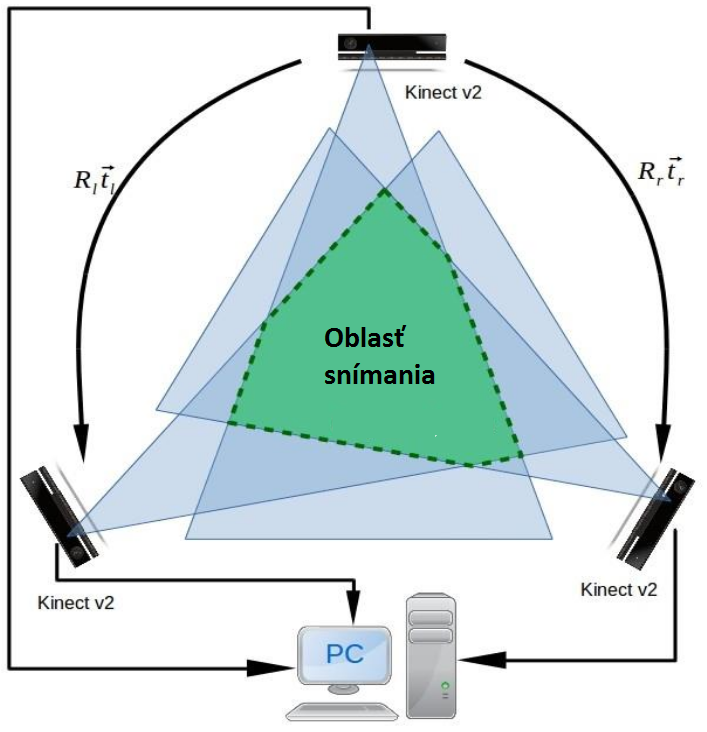
\includegraphics[width=0.55\textwidth]{figures/resers_m.png}
	\caption{Rekonštrukčný systém pozostávajúci z troch senzorov Kinect v2.}
	\label{fig:resers:m}
\end{figure}

V práci používali trojicu kamier Kinect v2 pripojených k jednému PC čo je rozdielny prístup oproti opísaným v \cite{7335499,6726991}. Pre odstránenie multi-kamerovej interferencie kamery pracovali v sekvenčnom režime. Kvalita hĺbkovej mapy je kľúčovým faktorom pri tvorbe a rekonštrukcii modelu. Ak sa v nej vyskytnú chyby, tie sa potom prenášajú do mračna bodov. Túto hĺbkovú mapu filtrovali použitím bilaterálneho filtra (BF) \cite{6272078}, \textit{Weight Median} filtra (WM) a \textit{Radius Outlier Removal} filtra (ROR). Vplyv filtračných metód na hĺbkovú mapu je zobrazený na obr. \ref{fig:resers:5}. Okrem toho tiež použili \textit{Weighted  Inter-Frame  Average} filter (WIFA), ktorý pracuje so sériou hĺbkových máp. Ten odstraňuje priestorový šum, ale výrazný pohyb robí aplikáciu WIFA nevhodnou pre vysoko dynamické scény \cite{6756961}.

\begin{figure}[H]
	\centering
	\begin{subfigure}[b]{0.24\textwidth}
		\centering
		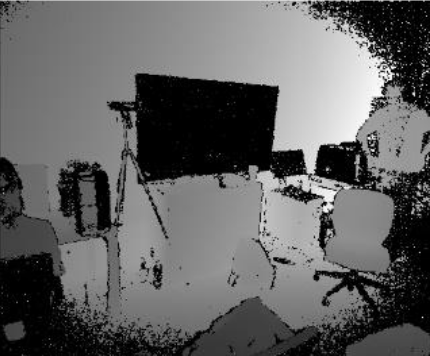
\includegraphics[width=\textwidth]{figures/resers_n.png}
		\caption{}
		\label{fig:resers:n}
	\end{subfigure}
	\hfill
	\begin{subfigure}[b]{0.24\textwidth}
		\centering
		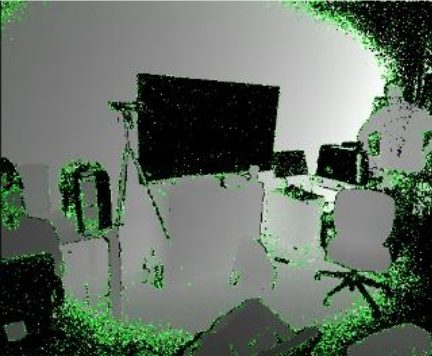
\includegraphics[width=\textwidth]{figures/resers_o.png}
		\caption{}
		\label{fig:resers:o}
	\end{subfigure}
	\hfill
	\begin{subfigure}[b]{0.24\textwidth}
		\centering
		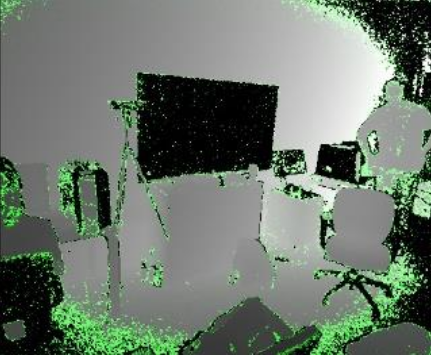
\includegraphics[width=\textwidth]{figures/resers_p.png}
		\caption{}
		\label{fig:resers:p}
	\end{subfigure}
	\hfill
	\begin{subfigure}[b]{0.24\textwidth}
		\centering
		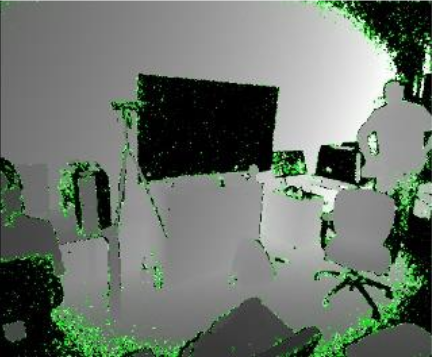
\includegraphics[width=\textwidth]{figures/resers_q.png}
		\caption{}
		\label{fig:resers:q}
	\end{subfigure}
	\caption{Výsledky filtrácie hĺbkovej mapy, kde zelená farba predstavuje rozdiely medzi prístupmi filtrácie: (\textbf{a}) Vstupná hĺbková mapa. 
		(\textbf{b}) Filtrácia pomocou BF.
		(\textbf{c}) Filtrácia pomocou BF + WM.
		(\textbf{d}) Filtrácia pomocou BF + WM + ROR \cite{satnik2018multiview}. }
	\label{fig:resers:5}
\end{figure}


Mračná bodov zo všetkých Kinect v2 sa následne spájajú do jedného mračna, čím sa vytvorí jednotná uniformná reprezentácia snímanej scény. Algoritmus rekonštrukcie sa používa na vytvorenie vernej a podrobnej reprezentácie povrchu skenovaných tvarov. V ďalšej fáze sa generuje trojuholníková sieť zachyteného 3D objektu. 


\begin{figure}[H]
	\centering
	\begin{subfigure}[b]{0.32\textwidth}
		\centering
		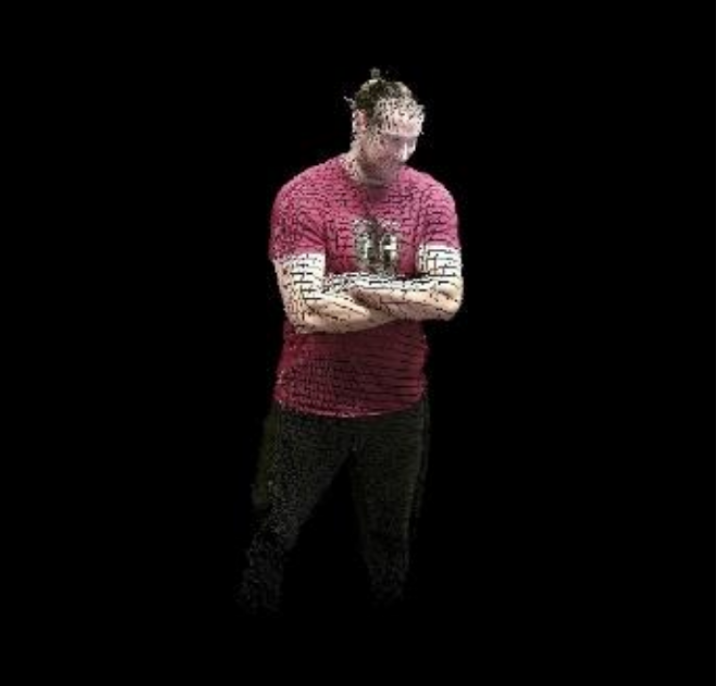
\includegraphics[width=\textwidth]{figures/resers_r.png}
		\caption{}
		\label{fig:resers:r}
	\end{subfigure}
	\hfill
	\begin{subfigure}[b]{0.315\textwidth}
		\centering
		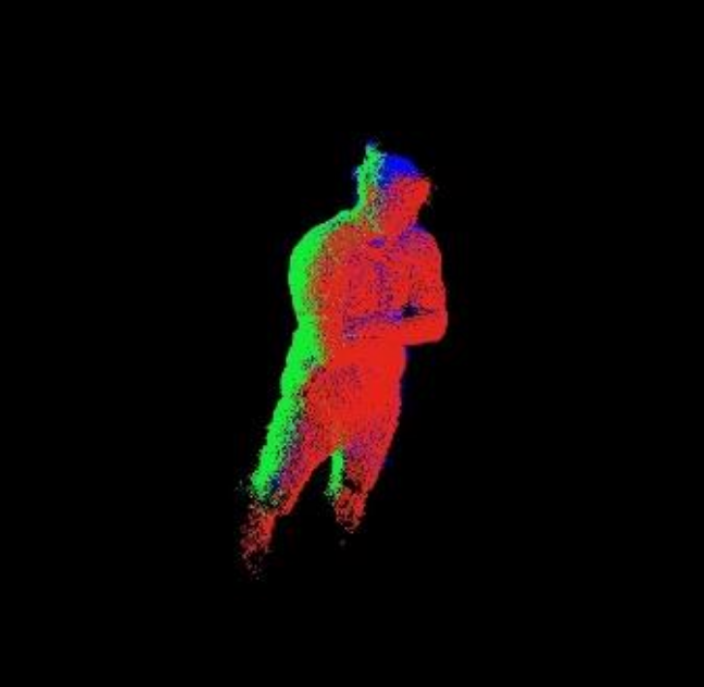
\includegraphics[width=\textwidth]{figures/resers_s.png}
		\caption{}
		\label{fig:resers:s}
	\end{subfigure}
	\hfill
	\begin{subfigure}[b]{0.32\textwidth}
		\centering
		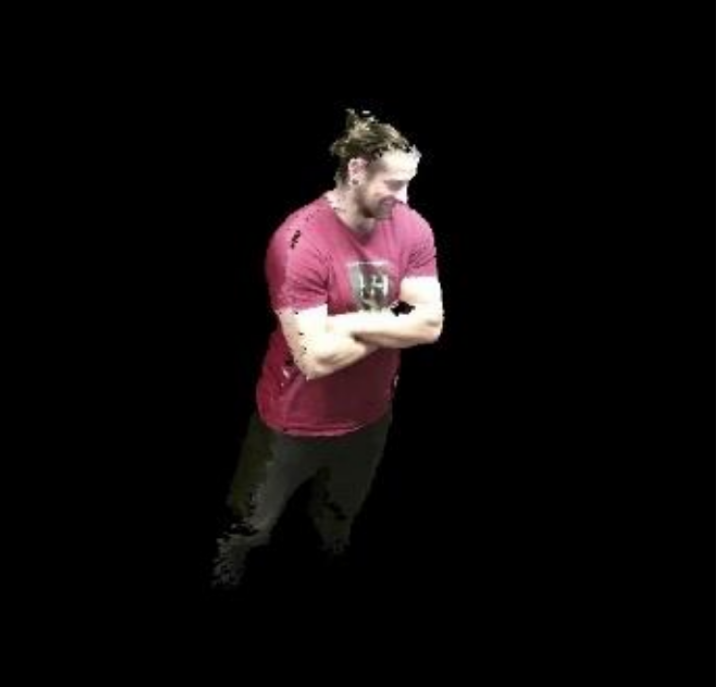
\includegraphics[width=\textwidth]{figures/resers_t.png}
		\caption{}
		\label{fig:resers:t}
	\end{subfigure}
	\caption{Rekonštrukcia scény z troch snímačov Kinect v2:
		(\textbf{a}) Mrak fúzovaných bodov generovaný každým snímačom Kinect.
		(\textbf{b}) Farebné oddelenie fúzovaných mračien bodov pre každú kameru.
		(\textbf{c}) Trojuholníková sieť vytvorená zo spojených mračien bodov \cite{satnik2018multiview}.}
	\label{fig:resers:6}
\end{figure}

V článku sa zamerali aj na meranie rýchlosti spracovania filtrácie. Pre prácu použili CUDA paralelné spracovanie na grafickej karte GeForce 780GTX. 
Meranie rýchlosti spracovania jednotlivých častí algoritmu sa vykonávalo na 400 hĺbkových mapách. Priemerný čas filtrácie so sieťovou rekonštrukciou trval 14,19ms. 

Autori predstavili návrh multi-kamerovej spolupráce 3 ToF snímačov značky Kinect v2. Bol opísaný spôsob kalibrácie a registrácie mračien bodov z jednotlivých kamier. Zároveň sa zamerali aj na filtráciu a trojuholníkovú rekonštrukciu snímaných objektov, pričom testovali rýchlosť spracovania.

%\subsection{VSR metóda pre registráciu mračien bodov z kamier Kinect }
%
%V článku \textit{A voxelize structured refinement method for registration of point clouds from Kinect sensors} sa autori zaoberajú rekonštrukciou mračien bodov pomocou jednej kamery Kinect. \cite{ozbay2019voxelize}. 

\newpage

\section{Disparitná a hĺbková mapa}


Výstupný obraz zachytávajúci vzdialenosť je závislý od použitej technológie snímania. Výstupom kamery je buď disparitná alebo hĺbková mapa \cite{davies2004machine}. Disparita zachytáva relatívnu vzdialenosť navzájom si odpovedajúcich bodov v stereo-páre
obrazu. Pri vytváraní disparity sa predpokladá s nulovou vertikálnou paralaxou. K výpočtu je teda potrebné mať dvojicu obrazov v epipolárnej rovine. Ak bod $x_1$ v ľavom obraze na pozícii [20,0] odpovedá v pravom obraze bodu $x_2$ [10,0], hodnota disparity $D$ má hodnotu 10. Pri výpočte sa jeden obraz zo stereo-páru berie ako referenčný.  
	
\begin{equation}
\label{eq:disp}
\begin{aligned}
D=x_1-x_2
\end{aligned}
\end{equation}

V disparitnej mape každý pixel nesie informáciu o disparite. Zobrazením vzniká obraz v odtieňoch sivej, ktorý vytvára ucelenú informáciu o priestore. Disparitná mapa je vždy vytváraná pre jeden obraz z dvojice, ktorej pozícia bodu sa berie ako referencia. Takáto mapa je už pre aplikáciu v stereovízií užitočná, pretože je z nej možné odlíšiť rozloženie snímanej scény. Neposkytuje však informáciu o reálnej vzdialenosti.

Hĺbková mapa je taktiež šedo-tónový obraz, ktorý zachytáva informáciu o absolútnej vzdialenosti $Z$ snímanej scény od kamery. 

\begin{figure}[H]
	\centering
	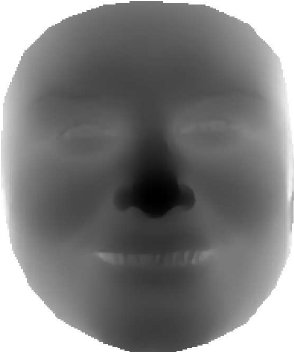
\includegraphics[height=4cm]{figures/depth_map.jpeg} 
	\caption{Ukážka hĺbkovej mapy povrchu tváre \cite{fabry2010surface}.}
	\label{fig:depth_map}
\end{figure}

\begin{equation}
\label{eq:depth}
\begin{aligned}
Z=\dfrac{bf}{x_1-x_2}=\dfrac{bf}{D}
\end{aligned}
\end{equation}

Pre výpočet je potrebné poznať rozostup medzi šošovkami kamier $b$ a ohniskovú vzdialenosť $f$. 

\newpage
\section{Princíp činnosti RGB-D kamier}
\label{sec:rgbd:principles}
RGB-D kamery sú optické snímače, ktoré zachytávajú hĺbkovú informáciu scény. Existuje viacero metód, ktorými tieto zariadenia pracujú. V tejto časti práce sú opísané najčastejšie používané metódy pre meranie hĺbky. \newline 

\begin{compactitem}
	\item \textbf{stereo-vízia:} ZED, Intel RealSense d415, stereo RGB
	\item \textbf{snímanie štrukturovaným svetlom (SLS):} Intel RealSense SR300 
	\item \textbf{meranie času doby letu (ToF):} Microsoft Kinect v2 
\end{compactitem}

\subsection{Stereovízia}

Metóda stereovízie je založená na synchronizovanom snímaní scény pomocou viacerých párov kamier (RGB alebo IR), ktoré sú voči sebe vzájomne posunuté. Najčastejšie rozloženia kamier sú Toe-In a Off-Axis, ktorá je znázornená na obr. \ref{fig:stereovizia}. Výstupom je farebný obraz scény zosnímanej z viacerých perspektív.

\begin{figure}[h]
	\centering
	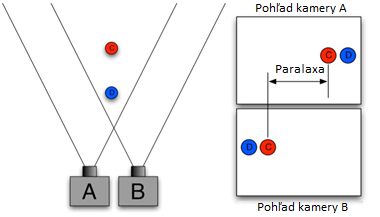
\includegraphics[width=0.6\textwidth]{figures/stereovizia.png} 
	\caption{Princíp stereovízie s Off-Axis nastavením kamier \cite{stereo}.}
	\label{fig:stereovizia}
\end{figure}

Na základe rozdielu z týchto dvoch perspektív a známych vonkajších parametrov stereo-kamerovej sústavy je možné dopočítať hĺbkový obraz \cite{kala2016road}. Hlavnou nevýhodou je vysoká výpočtová náročnosť algoritmu a cena kvalitných snímacích RGB senzorov. Taktiež je tento systém náchylný na meniace sa svetelné podmienky. Výhodou je nulová vzájomná interferencia.

\subsection{SLS snímače}
\label{sec:sls}
Structured Light Sensors (SLS) snímače sú zložené z projektora štrukturovaného svetla a snímača \cite{Geng}. Projektor aktívne osvecuje scénu so špeciálne navrhnutým 2D vzorom, častokrát priestorovo modulovaným svetlom. Kamera následne sníma osvetlenú scénu a získané dáta porovnáva s projektovaným vzorom. Ak je scéna planárna, snímaný vzor sa zhoduje s referenčným vzorom. Ak sú však v scéne povrchové variácie, geometrický tvar povrchu narúša projektované štrukturované svetlo. To sa následne nebude zhodovať s projektovaným vzorom.

\begin{figure}[H]
	\centering
	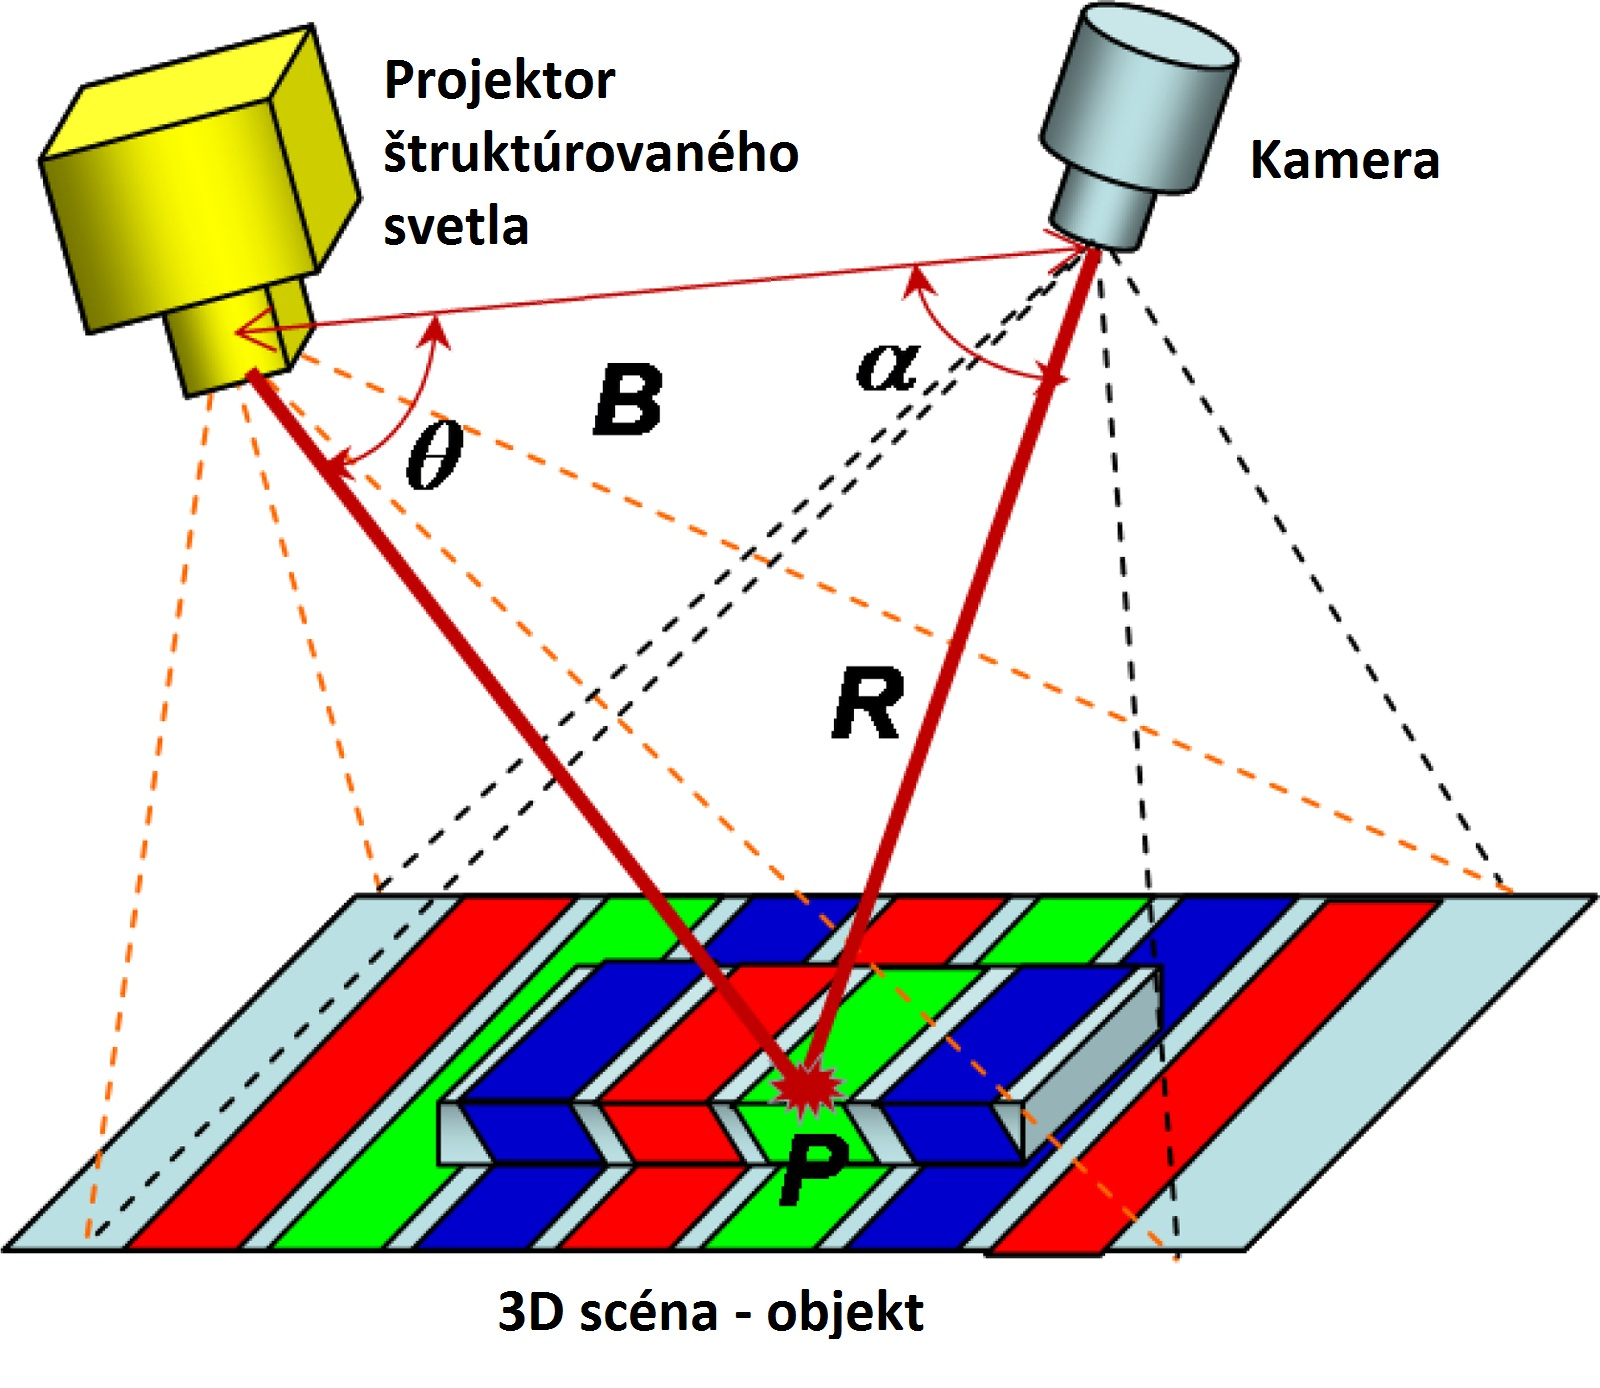
\includegraphics[width=0.47\textwidth]{figures/SLS.jpeg} 
	\caption{Princíp SLS kamery \cite{Geng}.}
	\label{fig:sls}
\end{figure}

Na obr. \ref{fig:sls} je znázornený geometrický vzťah medzi projektorom, kamerou a snímaným povrchom. Tento vzťah je možné vyjadriť triangulačným princípom:
\begin{equation}
\label{eq1}
\begin{aligned}
R=B\frac{\sin\theta}{\sin\alpha + \theta}
\end{aligned}
\end{equation}

Kľúčom k 3D zobrazovaniu na báze triangulačnej techniky je správne priradiť zosnímaný bod
k projekčnému bodu \cite{Geng}. Na tento účel boli navrhnuté rôzne schémy, ktoré sa delia na:

\begin{compactitem}
	\item \textbf{Sekvenčnú projekciu:} binárny kód, šedý kód, fázový posun, hybrid 
	\item \textbf{Priebežne meniacu projekciu:} dúhový kód, priebežne meniaci farebný kód 
	\item \textbf{Pásikový index:} farebne kódované pásy, segmentované pásy, De Bruijn, ...
	\item \textbf{Mriežkovaný index:} pseudo-náhodné binárne body, mini-vzor ako kód, ...
	\item \textbf{Hybridné metódy} 
\end{compactitem}

Hlavnou výhodou štruktúrovaného svetla je dosiahnutie vysokého priestorového rozlíšenia. Kamery pracujúce na tomto princípe nevyžadujú žiadnu špeciálnu úpravu na úrovni snímača. Akékoľvek rušenie je znázornené ako variácie v povrchu. Táto metóda snímania so sebou prináša problém multi-kamerovej interferencie. Tento fakt znemožňuje použitie týchto kamier v paralelnej spolupráci.



\subsection{ToF snímače}
\label{sec:tof}

Technológia \textit{Time of Flight} priniesla revolúciu v 3D strojovom videní, pretože umožňuje meranie hĺbky pomocou lacného CMOS chipu a aktívneho modulovaného sveta \cite{li2014time}. Kamera obsahuje zdroj IR svetla, ktorý je reprezentovaný polovodičovým laserom alebo LED s vlnovou dĺžkou $\sim$850nm. Vyžiarené svetlo sa odráža od snímaných objektov a spätne dopadá do prijímača IR svetla. Pre získanie vzdialenosti $d$ sa zisťuje fázový posun $\varphi$ medzi vyžiareným a prijatým signálom. Parameter $c$ predstavuje rýchlosť šírenia elektromagnetickej vlny v priestore. 

\begin{equation}
\label{eq2}
\begin{aligned}
d=\frac{c}{2}\frac{\Delta \varphi}{2 \pi f}
\end{aligned}
\end{equation}

Vyžiarené svetlo sa moduluje pulzne alebo kontinuálnou vlnou (continuous wave). Pulzná modulácia je bežnejšia kvôli ľahšej realizácii pomocou elektronických obvodov \cite{hansard2012time}. Na obr. \ref{fig:tof_principle} sa nachádza princíp detekcie hĺbky použitím ToF technológie so sínusovou moduláciou IR svetla \cite{van2006time}.

\begin{figure}[h]
	\centering
	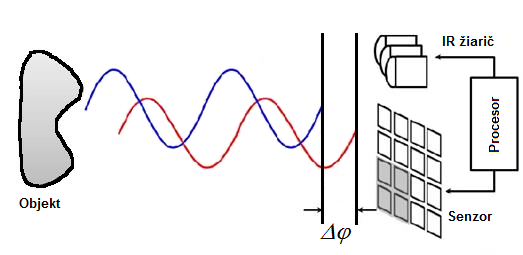
\includegraphics[width=0.65\textwidth]{figures/tof_principle.png} 
	\caption{Princíp činnosti ToF senzorov \cite{hansard2012time}.}
	\label{fig:tof_principle}
\end{figure}

Pri pulznej modulácii sa zdroj svetla rozsvecuje na dobu $\Delta t$. Odrazená energia sa paralelne vzorkuje pomocou dvoch vzorkovacích okien $C_1$ a $C_2$, ktoré sú fázovo posunuté o $180^\circ$. Elektrické náboje $Q_1$ a $Q_2$, akumulované počas doby vzorkovania, sa používajú pri výpočte vzdialenosti $d$ pomocou vzorca \ref{eq3}. Časový diagram pulznej modulácie sa nachádza na obr. \ref{fig:tof_principle_a}. 

\begin{equation}
\label{eq3}
\begin{aligned}
d=\frac{c}{2}\cdot\Delta t \left( \frac{Q_2}{Q_1 + Q_2}\right) 
\end{aligned}
\end{equation}


\begin{figure}[H]
	\centering
	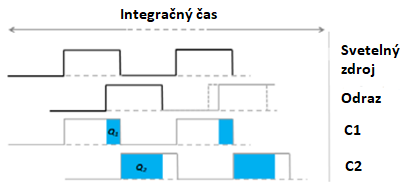
\includegraphics[width=0.65\textwidth]{figures/tof_principle_a.png} 
	\caption{Pulzná modulácia ToF senzora \cite{li2014time}.}
	\label{fig:tof_principle_a}
\end{figure}

Metóda s použitím kontinuálnej vlny (CW) využíva 4 vzorkovacie okna $C_1$ až $C_4$ posunuté voči sebe o $90^\circ$. Počas doby vzorkovania sa akumulujú náboje $Q$. Použitím tejto techniky je možné vypočítať fázový uhol $\varphi$ medzi prijatým a vyžiareným svetlom. Ten sa následne používa pre výpočet hĺbky. 

\begin{figure}[H]
	\centering
	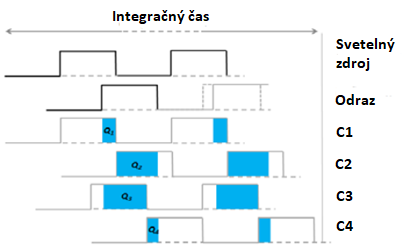
\includegraphics[width=0.65\textwidth]{figures/tof_principle_b.png} 
	\caption{Modulácia ToF senzora pomocou kontinuálnej vlny \cite{li2014time}.}
	\label{fig:tof_principle_b}
\end{figure}

\begin{equation}
\label{eq4}
\begin{aligned}
\varphi=\arctan \left( \frac{Q_3 - Q_4}{Q_1-Q_2} \right) 
\end{aligned}
\end{equation}

\begin{equation}
\label{eq:cw:depth}
\begin{aligned}
d=\dfrac{c}{4\pi f}\varphi 
\end{aligned}
\end{equation}

Pri CW modulácii sa z nameraných nábojov $Q_1$ až $Q_4$ vypočítava intenzita pixelu $A$ a ofset $B$. 

\begin{equation}
\label{eq5}
\begin{aligned}
A=\frac{\sqrt{\left(Q_1 - Q_2\right)^2 + \left(Q_3 - Q_4\right)^2 }} {2} 
\end{aligned}
\end{equation}

\begin{equation}
\label{eq6}
\begin{aligned}
B=\frac{Q_1 + Q_2 +Q_3 + Q_4}{4} 
\end{aligned}
\end{equation}

CW modulácia zabezpečuje zníženie chyby merania spôsobenej zmenou vnútorných parametrov elektronických komponentov. Napríklad zmena teploty kamery môže mať dopad na výsledné zosilnenie prijatých elektrických nábojov $Q$.V konečnom dôsledku to pri pulznej modulácií spôsobí nepresný výpočet hĺbky $d$ v rovnici \ref{eq3}. Pomocou parametrov $A$ a $B$ je možné aproximovať rozptyl hĺbky $\sigma$ \cite{li2014time}.

\begin{equation}
\label{eq7}
\begin{aligned}
\sigma=\frac{c}{4\sqrt{2 \pi f}} \frac{\sqrt{A+B}}{c_d A}
\end{aligned}
\end{equation}

Modulačný kontrast $ c_d $ opisuje ako efektívne ToF senzor separuje a zbiera prijaté fotoelektróny. Intenzita pixelu $ A $ je funkciou optického výkonu, $ B $ predstavuje ofset okolitého svetla a reziduálneho systému. Z tejto rovnice možno vyvodiť, že vysoká hodnota $A$, vysoká modulačná frekvencia frekvencia $f$ a vysoký modulačný kontrast zvyšujú presnosť merania. Naopak veľká úroveň ofsetu $B$ spôsobuje saturáciu prijímača a znižuje presnosť systému \cite{li2014time}. 

Medzi výhody ToF snímačov patrí zníženie vplyvu externého osvetlenia na kvalitu merania. Je to spôsobene tým, že nedochádza k ovplyvňovaniu frekvencie vyžarovaného svetla. Naopak pri použití viac-kamerového systému s rovnakou modulačnou frekvenciou môže dochádzať k vzájomnej interferencii signálov. Tento jav je detailne opísaný v kapitole \ref{kap:interference}.

\section{Mračno bodov a 3D povrch}

Hĺbková mapa zachytáva 3D priestor v 2D rovine. Tento obraz je získavaný z optických hĺbkových snímačov. Pre spätnú transformáciu hĺbkového obrazu do 3D priestoru sa jednotlivé obrazové pixely prevádzajú do takzvaných mračien bodov (anglicky Point Cloud). Základnou jednotkou mračna bodov je dátový bod, ktorý v sebe ukladá informáciu o polohe (x,y,z). Dátový bod môže v sebe uchovávať aj iné informácie ako napríklad farbu, jas, normálový vektor a podobne \cite{chua2017standards}. 

Takéto mračno bodov má veľké využitie v priemyselných 3D CAD modeloch, pri metrológií a inšpekcii kvality a v iných sférach, pretože reprezentuje geometrické vlastnosti reálnych objektov. 

\begin{figure}[!h]
	\centering
	\begin{subfigure}[b]{0.45\textwidth}
		\centering
		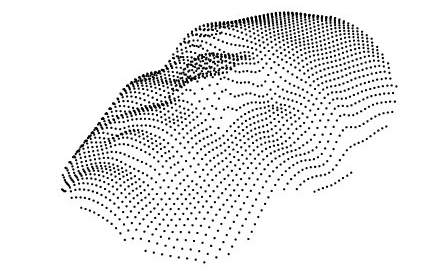
\includegraphics[height=4.5cm]{figures/point_cloud.jpeg}
		\caption{}
		\label{fig:point_cloud:a}
	\end{subfigure}
	\begin{subfigure}[b]{0.45\textwidth}
		\centering
		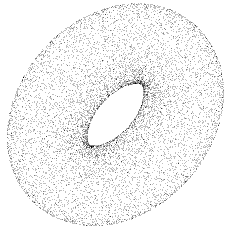
\includegraphics[height=4.5cm]{figures/point_cloud_b.png}
		\caption{}
		\label{fig:point_cloud:b}
	\end{subfigure}
	\caption{Mračno bodov: (\textbf{a}) Priestorová rekonštrukcia tváre vytvorenej z hĺbkovej mapy (Obr. \ref{fig:depth_map}) \cite{fabry2010surface}. (\textbf{b}) Priestorová rekonštrukcia torusu \cite{point_intel}. }
	\label{fig:point_cloud}
\end{figure}


Prevod mračna bodov na 3D povrch je realizovaný pomocou rekonštrukcie povrchu (\textit{surfacere construction}). Medzi známe rekonštrukčné metódy patrí Ball-Pivoting \cite{bernardini1999ball} a  Poissonova rekonštrukcia \cite{kazhdan2006poisson}, kde sú dátove body transformované do siete. Polygónová sieť je zložená z vertexov (vertices), hrán (edges) a masiek (faces), taktiež definuje tvar polyhedrálneho objektu v 3D grafike. Masky sa zvyčajne skladajú z trojuholníkov, štvorhranov a iných jednoduchých konvexných polygónov. Volumetrické siete explicitne reprezentujú povrch aj objem štruktúry, pričom polygónová sieť reprezentuje iba povrch. Objekty vytvorené z polygónov musia ukladať rôzne typy elementov. To zahŕňa vertexy, hrany, masky, polygóny a povrchy. Polygóny sú zvyčajne reprezentované trojuholníkmi \cite{smith2006vertex}. 

%\newpage
%\section{Spájanie a registrácia mračien bodov}
%
%Bodová registrácia tiež známa ako bodová zhoda je proces, pri ktorom sa hľadá priestorová transformácia zarovnávajúca dve mračná bodov. Účelom transformácie je zlúčenie viacerých mračien do jedného konzistentného modelu. Mračná môžu byť získané rôznymi typmi snímačov a rôznymi spôsobmi. Niektoré typy snímačov boli opísané v kapitole \ref{sec:rgbd:principles}. Pre získanie priestorovej transformácie existuje viacero algoritmov, ktoré sú opísané nižšie.


%\subsection{Problematika registrácie mračien bodov}
%
%Problematika registrácie mračien bola opísaná v práci „Robust Point Set Registration Using Gaussian Mixture Models„ \cite{jian2010robust}. Nech $\left\lbrace M, S \right\rbrace $ sú dva konečné mračná bodov v konečno-rozmernom reálnom vektorovom priestore. $M$ označuje pohyblivý modelový súbor a $S$ označuje statickú scénu. Obe množiny sa označujú ako podmnožiny konečno-priestorového vektora $\textbf{R}_{\textbf{d}}$ a môžu mať rozdielne veľkosti. Spoločným približovaním sa (registráciou) bodových množín $M$ a $S$ je možné odhadnúť mapovanie z $\textbf{R}_\textbf{d}$ do $\textbf{R}_\textbf{d}$ , čo prináša najlepšie zarovnanie medzi transformovanou a statickou sadou bodov. Transformačný model môže byť zapísaný ako $\textbf{T(M)}$ alebo $\textbf{T(M, $\theta$)}$, kde $\theta$ predstavuje optimalizačný parameter. Pri konvergencii bodov $M$ a $S$ je žiadané, aby vzdialenosť medzi zhodnými bodovými súbormi bola čo najmenšia. To je však bez vyskúšania všetkých transformácií ťažké, takže stačí lokálne minimum. Funkcia vzdialenosti medzi transformovaným dátovým setom a scénou $S$ je daná niektorou z funkcií $dist$. Jednoduchým spôsobom je výpočet štvorca euklidovskej vzdialenosti pre každý pár bodov:
%
%\begin{equation}
%\label{eq8}
%\begin{aligned}
%dist\left(T\left(M\right),S\right)=\sum_{m\epsilon T\left(M\right)} \sum_{s\epsilon S} \left(m-s\right)^2
%\end{aligned}
%\end{equation}
%
%\noindent Táto funkcia je náchylná voči šumovým dátam. Robustnosť $g$ sa môže docieliť M-estimátorom, ktorý dokáže odfiltrovať extrémne hodnoty \cite{tsin2004correlation}:
%
%\begin{equation}
%\label{eq9}
%\begin{aligned}
%dist_{robust}\left(T\left(M\right),S\right)=\sum_{m\epsilon T\left(M\right)} \sum_{s\epsilon S} g\left(m-s\right)^2
%\end{aligned}
%\end{equation}
%
%\subsection{Spôsoby registrácie mračien bodov}
%
%Spôsoby registrácie môžeme rozdeliť do dvoch kategórií. Prvou je tuhá (pevná alebo aj rigidná) a druhou pružná (elastická alebo aj nerigidna) registrácia. 
%
%\textbf{Pevná registrácia} využíva 6 stupňov voľnosti (6-DoF), pričom sa používajú afinné transformácie pre rotáciu a transláciu (sekcia \ref{sec:afine}). Táto transformácia je definovaná tak, že jednotlivé body nemenia euklidovskú vzdialenosť medzi sebou. 
%
%\textbf{Pružná registrácia} vzhľadom na dva bodové súbory prináša transformáciu, ktorá mapuje jednotlivé body na druhé. Využíva pritom aj nelineárne afinné transformácie. \newline
%
%\noindent Registračné metódy môžu byť rozdelené podľa aplikácie do týchto kategórií:
%
%\begin{compactitem}
%	\item Počiatočná registrácia 
%	\item Precízna registrácia
%	\item Globálna registrácia \newline
%\end{compactitem} 
%
%\noindent Taktiež ich delíme podľa princípu:
%\begin{compactitem}
%	\item Metódy založené na vzdialenostiach
%	\item Metódy založené na pravdepodobnosti
%	\item Metódy založené na filtrácií 
%	\item Metódy využívajúce spektrum
%	\item Metódy využívajúce strojové učenie \newline
%\end{compactitem}
%
%Pri počiatočnej registrácií sa hľadá prvotné zarovnanie 
%
%\noindent \textbf{Bodové registračné algoritmy}
%
%K bodovej registrácií sa používajú algoritmy, ktoré riešia všeobecnejší problém s porovnávaním grafov. Avšak výpočtová zložitosť zvykne byť vysoká a obmedzená na rigidné registrácie.\newline
%
%
%\noindent \textbf{Iterative closest point}
%
%ICP algoritmus je používaný na minimalizáciu rozdielu medzi dvoma mračnami bodov. Využíva sa na rekonštrukciu 2D a 3D povrchov, lokalizáciu robotov a podobne. Vykonáva rigidnú registráciu iteračným spôsobom za predpokladu, že každý bod v M korešponduje s najbližším bodom v S. V algoritme sa hľadá transformácia T pomocou metódy najmenších štvorcov.
%
%\begin{figure}[h]
%
%	\centering
%
%	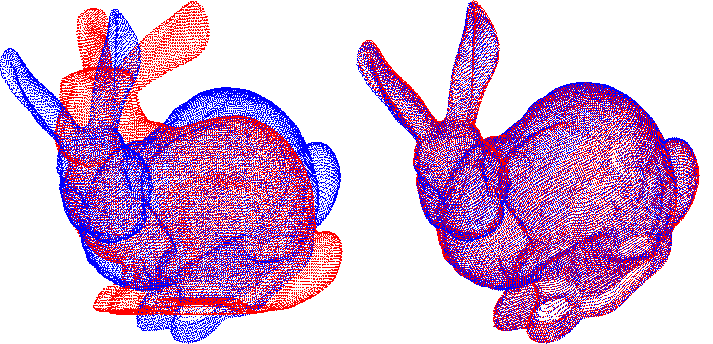
\includegraphics[width=0.7\textwidth]{figures/icp_principle.png} 
%
%	\caption{Ukážka registrácie mračien pomocou ICP algoritmu}
%	\label{fig:icp_principle}
%
%\end{figure}
%\newpage
%\textbf{Robustné párovanie bodov}
%
%Túto metódu (RPM) zaviedli Gold a kolektív (19). Táto metóda pracuje na zašumených 2D alebo 3D bodových setoch, ktoré môžu mať rozličné veľkosti a môžu sa líšiť pri voľných transformáciách. Pomocou kombinácie optimalizačných techník ako „deterministic annealing“ a „softassing“ , ktoré boli objavené pri rekurentných neurónových sieťach, sú analógové objektové funkcie popisujúce problémy minimalizované. Zatiaľ čo v ICP je korešpondencia vytvorená najbližším heuristickým binárnym systémom, RPM používa mäkkú korešpondenciu bodov. To znamená, že korešpondencia bodov môže byť ľubovoľná v rozmedzí 0 a 1. Zhoda v RPM je vždy jedna k jednej, čo pri ICP metóde nie je zabezpečené. Ak $m_i$ je i-ty bod množiny $M$ a $s_j$ je j-ty bod množiny $S$, tak matica zhody $\mu$ je definovaná ako:
%
%\begin{equation}
%\label{eq10}
%\begin{aligned}
%\mu_{ij}=
%\begin{cases}
%1, & \text{ak bod}\ m_i\ \text{korešponduje s bodom}\ s_j \\
%0, & \text{v inom prípade}
%\end{cases}
%\end{aligned}
%\end{equation}
%
%Riešením je nájsť afinnú transformáciu T , pri ktorej bude matica μ vykazovať najvyššiu zhodu (19). Znalosť optimálnej transformácie umožňuje ľahko určiť maticu zhody a naopak. Robustným párovaním bodov je možné určiť obe veci súčasne. Transformácia sa môže rozložiť na translačný vektor a transformačnú maticu.
%
%\begin{equation}
%\label{eq11}
%\begin{aligned}
%T\left(m\right)=\bar{A}m+\bar{t}
%\end{aligned}
%\end{equation}
%
%Matica \textbf{A} sa skladá zo štyroch samostatných parametrov $\left\lbrace a, \theta, b, c \right\rbrace$, ktoré spôsobujú zmenu veľkosti, rotáciu, horizontálnu a vertikálnu geometrickú transformáciu.
%
%\noindent Účelová funkcia je reprezentovaná rovnicou 3.12 pričom v nej platí podmienka 3.13:
%
%\begin{equation}
%\label{eq12}
%\begin{aligned}
%cost=\sum_{j=1}^{N}\sum_{i=1}^{M} \mu_{ij} \Arrowvert s_j - \boldsymbol{t} - \boldsymbol{Am_i} \Arrowvert^2 + \boldsymbol{g\left(A\right)} -\alpha \sum_{j=1}^{N}\sum_{i=1}^{M} \mu_{ij}
%\end{aligned}
%\end{equation}
%
%\begin{equation}
%\label{eq13}
%\begin{aligned}
%\forall j \sum_{i=1}^{M} \leq 1, \forall i \sum_{j=1}^{N} \mu_{ij} \leq 1, \forall ij \mu_{ij} \in \left\lbrace 0,1 \right\rbrace 
%\end{aligned}
%\end{equation}
%
%Parameter $\alpha$ ovplyvňuje funkciu k silnejšej korelácii. Funkcia $g\left(A\right)$ slúži na reguláciu afinnej transformácie penalizovaním veľkých hodnôt transformovaných komponentov. Pre niektoré regulačné parametre $\gamma$ platí $g\left(A\left(a, \theta, b, c\right)\right) = \gamma \left(a^2 + b^2 + c^2 \right)$. Táto metóda RPM optimalizuje hodnotovú funkciu použitím „Softassign“ algoritmu. \newline

%\textbf{Korelácia kernelu}
%
%Metóda korelácie kernelu (KC) je oproti ICP metóde odolnejšia voči zašumeným dátam. Na rozdiel od ICP, v tejto metóde každý bod scény uvažuje s modelovým bodom. Ide o viacnásobne prepojujúcu registráciu (18). Pre niektoré funkcie kernelu $K$ je KC dvoch bodov $\chi_i$ a $\chi_j$ definovaná nasledovne:
%
%\begin{equation}
%\label{eq14}
%\begin{aligned}
%KC\left(\chi_i,x_j\right)=\int K\left(\chi,\chi_i\right) \cdot K\left(\chi,\chi_j\right) dx 
%\end{aligned}
%\end{equation}
%
%Funkcia K zvolená pre bodovú registráciu je typický symetrický a nenegatívný kernel. Zvyčajne je používaný Gaussov kernel pre svoju jednoduchosť, avšak časté sú aj \textit{Epanechnikov} a \textit{tricube} kernel (18). Korelácia kernelu celej množiny bodov χ je definovaná ako súčet korelácií kernelu každého bodu v množine s každým ďalším bodom v množine.
%
%
%\begin{equation}
%\label{eq15}
%\begin{aligned}
%KC\left(\chi\right) = \sum_{i\ne1} KC\left(\chi_i,\chi_j\right)=2\sum_{i<j} KC\left(\chi_i,\chi_j\right)
%\end{aligned}
%\end{equation}
%
%Hodnota $KC$ množiny bodov je proporcionálna v rámci konštantného faktora logaritmu informačnej entropie. $KC$ je v podstate mierou kompaktnosti bodu, ktorý je triviálne nastavený. Ak by sa všetky body nachádzali v jednom mieste, $KC$ by nadobudol veľkú hodnotu. Účelová funkcia ($cost$) dátovej množiny pre určité transformačné parametre $\theta$ je definovaná nasledovne :
%
%\begin{equation}
%\label{eq16}
%\begin{aligned}
%cost\left(S,M,\theta\right)= - \sum_{m\in M} \sum_{s\in S} KC \left(s, T\left(m, \theta \right)\right)
%\end{aligned}
%\end{equation}
%
%Niektoré algebrické manipulácie sú opísané rovnicou 3.17:
%
%\begin{equation}
%\label{eq17}
%\begin{aligned}
%KC\left(S\cup T\left(M,\theta\right)\right) = KC\left(S\right) + KC\left(T \left(M, \theta \right)\right) - 2cost\left(S,M,\theta \right)
%\end{aligned}
%\end{equation}
%
%Výraz je zjednodušený tým, že sa pozoruje $KC\left(S\right)$ nezávisle od $\theta$. Ak sa ešte uvažuje s rigidnou registráciou, $KC\left(T \left(M, \theta \right)\right)$ je tým pádom invariantný voči zmene $\theta$, pretože Euklidovská vzdialenosť medzi párom bodov sa pri rigidnej transformácii nemení. Tým pádom je rovnicu 3.17 možné prepísať na 3.18:
%
%\begin{equation}
%\label{eq18}
%\begin{aligned}
%KC\left(S\cup T\left(M,\theta\right)\right) = c - 2cost\left(S,M,\theta \right)
%\end{aligned}
%\end{equation}
%
%
%Estimácia hustoty kernelu je neparametrický spôsob odhadovania hustoty pravdepodobnosti náhodnej premennej. Odhad hustoty kernelu je základným problémom vyhladzovania údajov na základe dátovej vzorky. Jej definícia pre tento prípad je znázornená v rovniciach 3.19 a 3.20.
%
%\begin{equation}
%\label{eq19}
%\begin{aligned}
%P_M\left( \chi,\theta\right)=\frac{1}{M}\sum_{m\in M} K\left(\chi,T\left(m,\theta\right)\right)
%\end{aligned}
%\end{equation}
%
%\begin{equation}
%\label{eq20}
%\begin{aligned}
%P_S\left( \chi\right)=\frac{1}{N}\sum_{s\in S} K\left(\chi,s\right)
%\end{aligned}
%\end{equation}
%
%Účelovú funkciu následne možno dokázať ako koreláciu odhadov hustoty kernelu.
%
%\begin{equation}
%\label{eq21}
%\begin{aligned}
%cost\left(S,M,\theta\right)= - N^2 \int_{\chi} \left(P_M P_s\right)
%\end{aligned}
%\end{equation}
%
%Po získaní hodnotovej funkcie algoritmus používa zostup gradientu, čo je iteračný optimalizačný algoritmus prvého radu na zistenie minimálnej funkcie. Ním sa nachádza optimálna transformácia. Z dôvodu výpočtovej náročnosti sa používa diskrétna verzia funkcie\textbf{ 3.18}. Oproti ICP algoritmu KC metóda nepotrebuje nájsť najbližšieho suseda a tým pádom je ľahšia na implementáciu. Taktiež je menej náchylná na šum v dátach (18).


	\chapter{Kalibrácia kamier} 
\label{kap:kalibracia}
\pagestyle{fancy}
\fancyhf{}
\fancyfoot[CE,CO]{\thepage}
\renewcommand{\footrulewidth}{1pt}
\lhead{Kalibrácia kamier}

% Richard Hartley and Andrew Zisserman. Multiple view geometry in computer vision. Cambridge university press, 2003.
% http://www.programmersought.com/article/5593383746/
% https://en.wikipedia.org/wiki/Pinhole_camera_model
% http://www.cse.psu.edu/~rtc12/CSE486/lecture13.pdf
% https://docs.opencv.org/2.4/modules/calib3d/doc/camera_calibration_and_3d_reconstruction.html

Kamera je nástroj, ktorý mapuje 3D priestor do 2D roviny obrazu. Ide o technické zariadenie, ktoré je využívané širokospektrálne. Existuje viacero technologických riešení a produktov, ktoré sú špecifikované na konkrétne aplikácie. Pri potrebe merania vzdialenosti alebo zachytenia presnej hĺbkovej informácie snímanej scény je potrebné uvažovať s kalibráciou kamery. 

Geometrická kalibrácia je nevyhnutá z dôvodu skreslenia šošovky, čo spôsobuje výrazné nepresnosti pri transformácii 3D priestoru 2D obrazovej roviny. Pri kalibrácii je dôležité poznať matematický model kamery a transformácie, ktorými sa upravuje výsledný obraz. 

Pri multi-kamerovej kalibrácii hľadáme vzájomnú polohu kamier vo svetových súradniciach. Ak je aplikácia zameraná na 3D rekonštrukciu priestoru z viacerých kamier, vzájomnou kalibráciu vieme ľahšie spojiť pohľady do jedného spoločného zosúladeného priestoru. 


\section{Afinné transformácie v priestore}
\label{sec:afine}
%http://fractal.dam.fmph.uniba.sk/~batorova/UPG/2_Transformacie
%http://www.sccg.sk/~pilnikova/pg/afinne_transformacie.pdf
%https://www.mathworks.com/discovery/affine-transformation.html


Afinná transformácia je metóda lineárneho mapovania, ktorá zachováva body, priame čiary a roviny. Množiny rovnobežných čiar zostávajú po afinnej transformácii rovnobežné. Technika afinitnej transformácie sa zvyčajne používa na korekciu geometrických skreslení alebo deformácií, ktoré sa vyskytujú pri neideálnych uhloch kamery. Matematický zápis afinnej transformácie je $X'=A\cdot X$, kde $X$ predstavuje pôvodnú súradnicu bodu, $X'$ transformovanú súradnicu bodu a $A$ danú afinnú transformáciu. Afinná transformácia pre 3D priestor má tvar matice o rozmere $4\times 4$.\newline

\textbf{\textit{Identická transformácia:}} Určená jednotkovou maticou, body $X$ a $X'$ majú totožné súradnice. 

\begin{equation}
\label{eq_kalib_ident}
\begin{aligned}
\begin{bmatrix}
x' \\ y' \\ z' \\ 1
\end{bmatrix}=
\begin{bmatrix}
1 & 0 & 0 & 0 \\
0 & 1 & 0 & 0 \\
0 & 0 & 1 & 0 \\
0 & 0 & 0 & 1 
\end{bmatrix}
\begin{bmatrix}
x \\ y \\ z \\ 1 
\end{bmatrix}
\end{aligned}
\end{equation}

\textbf{\textit{Translačná transformácia:}} Posun bodu $X$ o vektor $\vec{a}=\left[a_x,a_y,a_z\right]$, $X'= \vec{a} + X$.

\begin{equation}
\label{eq_kalib_translat}
\begin{aligned}
\begin{bmatrix}
x' \\ y' \\ z' \\ 1 
\end{bmatrix}
=
\begin{bmatrix}
1 & 0 & 0 & a_x \\
0 & 1 & 0 & a_y \\
0 & 0 & 1 & a_z \\
0 & 0 & 0 & 1 
\end{bmatrix}
\begin{bmatrix}
x \\ y \\ z \\ 1 
\end{bmatrix}
\end{aligned}
\end{equation}


\textbf{\textit{Škálovacia transformácia:}} Zmena  bodu $X$ o vektor $\vec{a}=\left[a_x,a_y,a_z\right]$, $X'= \vec{a}X$.

\begin{equation}
\label{eq_kalib_scale}
\begin{aligned}
\begin{bmatrix}
x' \\ y' \\ z' \\ 1 
\end{bmatrix}
=
\begin{bmatrix}
s_x & 0 & 0 & 0 \\
0 & s_y & 0 & 0 \\
0 & 0 & s_z & 0 \\
0 & 0 & 0 & 1 
\end{bmatrix}
\begin{bmatrix}
x \\ y \\ z \\ 1 
\end{bmatrix}
\end{aligned}
\end{equation}

\textbf{\textit{Rotačná transformácia v osi x:}}  Otočenie bodu X okolo začiatku súradnicovej sústavy o uhol $\alpha$.

\begin{equation}
\label{eq_kalib_rotat_x}
\begin{aligned}
\begin{bmatrix}
x' \\ y' \\ z' \\ 1 
\end{bmatrix}
=
\begin{bmatrix}
1 & 0 & 0 & 0 \\
0 & \cos\alpha & -\sin\alpha & 0 \\
0 & \sin\alpha & \cos\alpha & 0 \\
0 & 0 & 0 & 1 
\end{bmatrix}
\begin{bmatrix}
x \\ y \\ z \\ 1 
\end{bmatrix}
\end{aligned}
\end{equation}

\newpage
\textbf{\textit{Rotačná transformácia v osi y:}}  Otočenie bodu X okolo začiatku súradnicovej sústavy o uhol $\alpha$.

\begin{equation}
\label{eq_kalib_rotat_y}
\begin{aligned}
\begin{bmatrix}
x' \\ y' \\ z' \\ 1 
\end{bmatrix}
=
\begin{bmatrix}
\cos\alpha & 0 & \sin\alpha & 0 \\
0 & 1 & 0 & 0 \\
-\sin\alpha & 0 & \cos\alpha & 0 \\
0 & 0 & 0 & 1 
\end{bmatrix}
\begin{bmatrix}
x \\ y \\ z \\ 1 
\end{bmatrix}
\end{aligned}
\end{equation}


\textbf{\textit{Rotačná transformácia v osi z:}} Otočenie bodu X okolo začiatku súradnicovej sústavy o uhol $\alpha$ .

\begin{equation}
\label{eq_kalib_rotat_z}
\begin{aligned}
\begin{bmatrix}
x' \\ y' \\ z' \\ 1 
\end{bmatrix}
=
\begin{bmatrix}
\cos\alpha & -\sin\alpha & 0 & 0  \\
\sin\alpha & \cos\alpha & 0 & 0 \\
0 & 0 & 0 & 0 \\
0 & 0 & 0 & 1 
\end{bmatrix}
\begin{bmatrix}
x \\ y \\ z \\ 1 
\end{bmatrix}
\end{aligned}
\end{equation}

\textbf{\textit{Súmerná transformácia v osi x:}} Matica súmernosti vzhľadom na os x.

\begin{equation}
\label{eq_kalib_sumer_x}
\begin{aligned}
\begin{bmatrix}
x' \\ y' \\ z' \\ 1 
\end{bmatrix}
=
\begin{bmatrix}
-1 & 0 & 0 & 0 \\
0 & 1 & 0 & 0 \\
0 & 0 & 1 & 0 \\
0 & 0 & 0 & 1 
\end{bmatrix}
\begin{bmatrix}
x \\ y \\ z \\ 1 
\end{bmatrix}
\end{aligned}
\end{equation}

\textbf{\textit{Súmerná transformácia v osi y:}} Matica súmernosti vzhľadom na os y.

\begin{equation}
\label{eq_kalib_sumer_y}
\begin{aligned}
\begin{bmatrix}
x' \\ y' \\ z' \\ 1 
\end{bmatrix}
=
\begin{bmatrix}
1 & 0 & 0 & 0 \\
0 & -1 & 0 & 0 \\
0 & 0 & 1 & 0 \\
0 & 0 & 0 & 1 
\end{bmatrix}
\begin{bmatrix}
x \\ y \\ z \\ 1 
\end{bmatrix}
\end{aligned}
\end{equation}

\textbf{\textit{Súmerná transformácia v osi z:}} Matica súmernosti vzhľadom na os z. 

\begin{equation}
\label{eq_kalib_sumer_z}
\begin{aligned}
\begin{bmatrix}
x' \\ y' \\ z' \\ 1 
\end{bmatrix}
=
\begin{bmatrix}
1 & 0 & 0 & 0 \\
0 & 1 & 0 & 0 \\
0 & 0 & -1 & 0 \\
0 & 0 & 0 & 1 
\end{bmatrix}
\begin{bmatrix}
x \\ y \\ z \\ 1 
\end{bmatrix}
\end{aligned}
\end{equation}




\section{Dierková kamera}
Dierková kamera (pinhole camera) predstavuje ideálnu kameru, ktorá nevykazuje žiadne skreslenia spôsobené šošovkou. Ide o najjednoduchší model kamery, ktorým svetlo namiesto šošovky prechádza cez štrbinu a prevrátené dopadá na rovinu obrazu. Dochádza tu k centrálnej projekcii bodov zo svetových súradníc do roviny obrazu.

\begin{figure}[h]
	\centering
	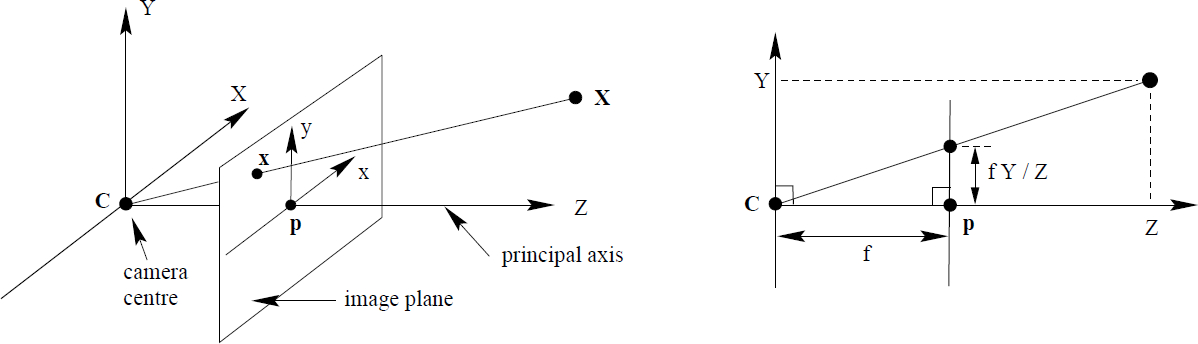
\includegraphics[width=\textwidth]{figures/pinhole_camera.jpg} 
	\caption{Perspektívna projekcia štrbinovou kamerou.}
	\label{fig:pinhole_camera}
\end{figure}

Na obrázku \ref{fig:pinhole_camera} je znázornená geometria dierkovej kamery. Stredom projekcie je optické centrum. Kolmica medzi optickým centrom a obrazovou rovinu $\pi$ sa nazýva hlavná os $Z$. Hlavným bodom $p$ je miesto, v ktorom os $Z$ pretína obrazovú rovinu. Rovina prechádzajúca stredom kamery rovnobežne s rovinou obrazu sa nazýva hlavná rovina kamery. $C$ reprezentuje stred kamery (stred perspektívneho premietania). Za predpokladu, že svetové a obrazové body sú zastúpené v homogénnych súradniciach, potom sa stredná projekcia môže jednoducho vyjadriť ako lineárne mapovanie medzi ich homogénnymi súradnicami.

\begin{figure}[h]
	\centering
	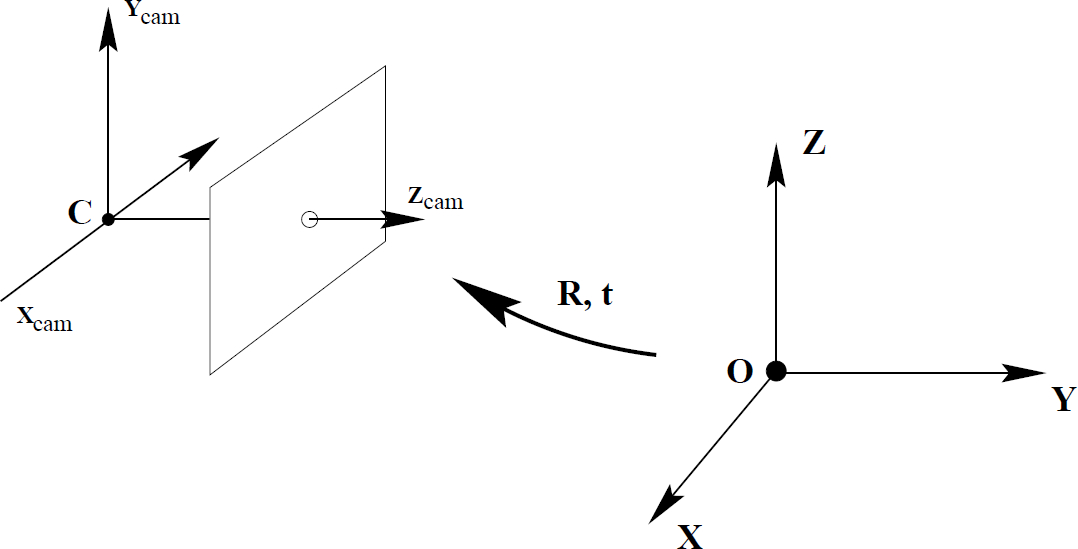
\includegraphics[width=0.7\textwidth]{figures/rotat_translat.jpg} 
	\caption{Vzťah medzi svetovou súradnicovou sústavou a súradnicovou sústavou kamery.}
	\label{fig:rotat_translat}
\end{figure}

Prevod medzi svetovou súradnicovou sústavou (SSS) a kamerovou súradnicovou sústavou (KSS) je zobrazený na obr. \ref{fig:rotat_translat} predstavený vzťahom \ref{eq::pinhole::world_camera}.\newline 

\begin{equation}
\label{eq::pinhole::world_camera}
\begin{aligned}
\begin{bmatrix}
X_{cam} \\ Y_{cam} \\ Z_{cam} \\ 1
\end{bmatrix}=
\boldsymbol{RT}
\begin{bmatrix}
X \\ Y \\ Z \\ 1
\end{bmatrix}
\end{aligned}
\end{equation}

\newpage
\textbf{Svetová súradnicová sústava} je reprezentovaná trojrozmerným karteziánskym súradnicovým systémom, kde stred sústavy $O$ (prípadne $O_w$) je v bode [0,0,0]. Vektory $X,Y,Z$ prislúchajúce k jednotlivým súradniciam sú na seba kolmé. Definujú polohu objektu v scéne. Udávajú sa v dĺžkových jednotkách $[m]$ alebo $[mm]$.\newline 

\textbf{Súradnicová sústava kamery} je reprezentovaná trojrozmerným súradnicovým systémom v bode $C$ (poprípade $O_c$), čo predstavuje stred kamery. Optická os $Z_c$ je daná vektorom pohľadu kamery. Vzťah medzi svetovou súradnicovou sústavou a súradnicovou sústavou kamery je popísaný transláciou $t$ a rotáciou $R$. Vektory sú označené ako $(X_{cam},Y_{cam},Z_{cam})$ \newline 

Body zo súradnicovej sústavy kamery je následne potrebné premietnuť do roviny obrazu $\pi$. Nech je stred premietania pôvodom euklidovského súradnicového systému a obrazová (ohnisková) rovina $Z=f$. Podľa modelu dierkovej kamery na obr. \ref{fig:pinhole_camera} sa bod v priestore so súradnicami $\left(X,Y,Z\right)^T$ mapuje na bod v rovine obrazu $\left(f\frac{X}{Z}, f\frac{Y}{Z}, f \right)^T$ pomocou podobnosti trojuholníkov. Ignorovaním výsledných súradníc obrazu dostávame vzťah ktorý popisuje mapovanie centrálnej projekcie zo svetovej súradnicovej sústavy do obrazovej súradnicovej sústavy.

\begin{equation}
\label{eq::pinhole::camera_iplane::a}
\begin{aligned}
\frac{X_{cam}}{x}=\frac{Z_{cam}}{f}; \frac{Y_{cam}}{y}=\frac{Z_{cam}}{f}
\end{aligned}
\end{equation}

\begin{equation}
\label{eq::pinhole::camera_iplane::b}
\begin{aligned}
x=f\frac{X_{cam}}{Z_{cam}}; y=f\frac{Y_{cam}}{Z_{cam}}
\end{aligned}
\end{equation}

Rovnice \ref{eq::pinhole::camera_iplane::a} a \ref{eq::pinhole::camera_iplane::a} môžeme prepísať do maticového tvaru

\begin{equation}
\label{eq::pinhole::camera_iplane}
\begin{aligned}
\begin{bmatrix}
fX_{cam} \\ fY_{cam} \\ Z_{cam}
\end{bmatrix}
= Z_{cam}
\begin{bmatrix}
x \\ y \\ 1
\end{bmatrix}
=
\begin{bmatrix}
f & 0 & 0 & 0 \\
0 & f & 0 & 0 \\
0 & 0 & 1 & 0 \\
\end{bmatrix}
\begin{bmatrix}
X_{cam} \\ Y_{cam} \\ Z_{cam} \\ 1 
\end{bmatrix}
\end{aligned}
\end{equation}

\textbf{Rovina obrazu} aj \textbf{súradnicový systém obrazových bodov} predstavuje dvojrozmerný priestor. Rozdielom je, že prvý spomenutý systém má počiatok v hlavnom bode a jednotka súradnicového systému je v milimetroch. Druhý spomenutý je reprezentovaný jednotkou pixel, počiatok súradnicového systému je na pozícii $\left(u,v\right)=\left[0,0\right]$. Preto je potrebné transformovať prvý súradnicový systém do druhého. 

\begin{figure}[h]
	\centering
	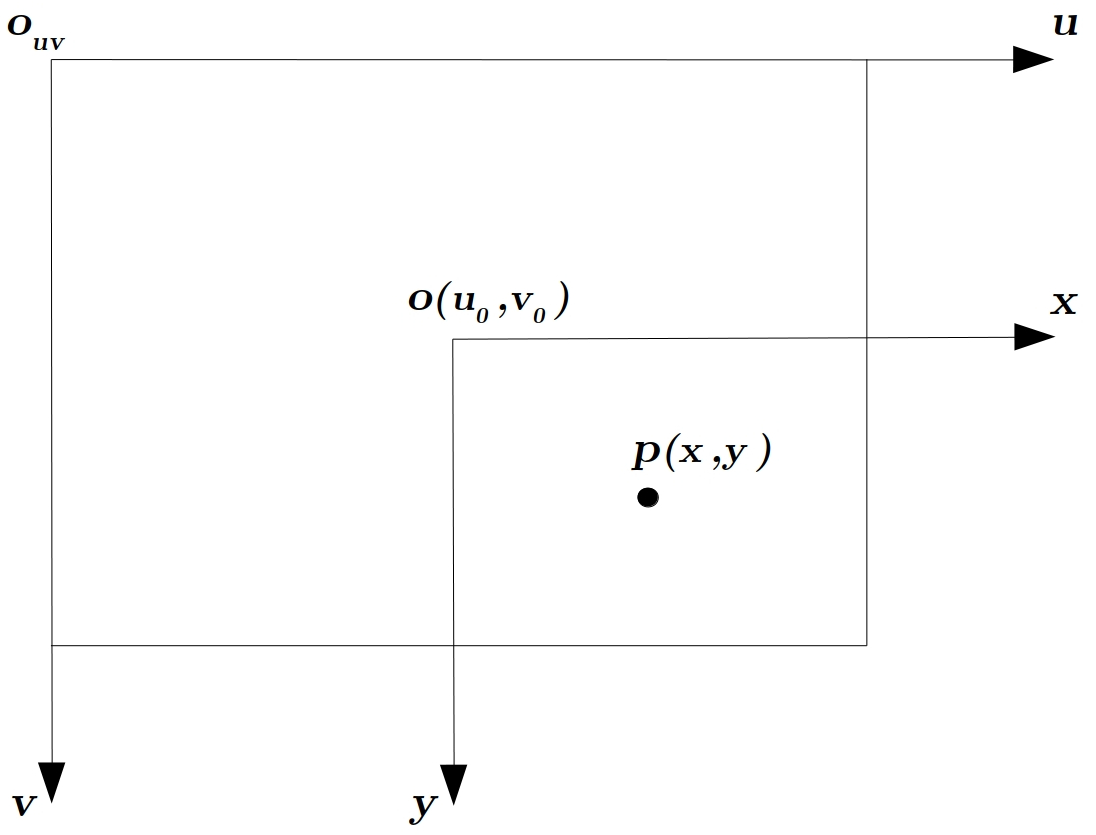
\includegraphics[width=0.45\textwidth]{figures/plane_pixel.jpg} 
	\caption{Vzťah roviny obrazu a súradnicového systému obrazových bodov.}
	\label{fig:plane_pixel}
\end{figure}

Z obr. \ref{fig:plane_pixel} je definovaný hlavný bod $p=o(u_0,v_0)$ (bod, ktorým prechádza hlavná os $Z_{cam}$ v obr. \ref{fig:pinhole_camera}). Pre prevod potrebujeme poznať hustotu pixelov na jednotku dĺžky. Tá je určená pomerom počtu pixelov a rozmerom snímacej plochy v jednotlivých smeroch. Pridaním offsetu $u_0$ a $v_0$ dostávame transformačný vzťah

\begin{equation}
\label{eq::pinhole::plane_pixel}
\begin{aligned}
u=\frac{x}{d_x} + u_0; v=\frac{y}{d_x} + v_0
\end{aligned}
\end{equation}

Z rovnice \ref{eq::pinhole::plane_pixel} získavame kalibračnú maticu $K$, ktorá je zložená z ohniskových vzdialeností $f_x, f_y$ a hlavných bodov $p_x, p_y$. Do úplnej matice $K$ patrí aj koeficient skosenia $s$, ktorý je zvyčajne 0. Táto matica je zložená z takzvaných vnútorných parametrov kamery.

\begin{equation}
\label{eq::pinhole::intrinsic}
\begin{aligned}
K=
\begin{bmatrix}
\frac{x}{d_x} & s & u_0 \\
0 & \frac{y}{d_y} & v_0 \\
0 & 0 & 1 \\
\end{bmatrix}
\begin{bmatrix}
f & 0 & 0 & 0 \\
0 & f & 0 & 0 \\
0 & 0 & 1 & 0 \\
\end{bmatrix}
=
\begin{bmatrix}
f_x & s & p_x & 0 \\
0 & f_y & p_y & 0 \\
0 & 0 & 1 & 0 \\
\end{bmatrix}
\end{aligned}
\end{equation}

Matica kamery $P$ sa skladá z vnútorných a vonkajších parametrov. Matica $R$ zastupuje rotáciu a $t$ transláciu, čo sú vonkajšie parametre (obr. \ref{fig:rotat_translat}). Matica $K$ zastupuje vnútorné parametre.

\begin{equation}
\label{eq::pinhole::p}
\begin{aligned}
\boldsymbol{P}=
\boldsymbol{
K
\begin{bmatrix}
R & t
\end{bmatrix}}=
\begin{bmatrix}
f_x & 0 & p_x \\
0 & f_y & p_y \\
0 & 0 & 1 \\
\end{bmatrix}
\begin{bmatrix}
r_{11} & r_{12} & r_{13} & t_{1} \\
r_{21} & r_{22} & r_{23} & t_{2} \\
r_{31} & r_{32} & r_{33} & t_{3} \\
\end{bmatrix}
\end{aligned}
\end{equation}

Celý prevod je teda možné vyjadriť podľa rovnice \ref{eq::pinhole::full} 
\begin{equation}
\label{eq::pinhole::full}
\begin{aligned}
Z_{cam}
\begin{bmatrix}
u \\ v \\ 1
\end{bmatrix}
=
\begin{bmatrix}
f_x & 0 & p_x \\
0 & f_y & p_y \\
0 & 0 & 1 \\
\end{bmatrix}
\begin{bmatrix}
r_{11} & r_{12} & r_{13} & t_{1} \\
r_{21} & r_{22} & r_{23} & t_{2} \\
r_{31} & r_{32} & r_{33} & t_{3} \\
\end{bmatrix}
\begin{bmatrix}
X \\ Y \\ Z \\ 1
\end{bmatrix}
\end{aligned}
\end{equation}

ktorá je základným matematickým opisom dierkovej kamery a prevodu svetových súradníc do súradnicového systému obrazových bodov. 

\section{Skreslenie šošoviek}

V reálnych kamerách sa vyskytujú určité typy nelineárneho skreslenia, ktoré sú spôsobené pridaním šošovky do ideálnej kamery. Tieto skreslenia spôsobujú nesprávnu perspektívnu projekciu, čím sa následne stráca presná informácia o snímanej scéne. Tieto skreslenia je však možné odstrániť získaním vnútorných parametrov kamery. Medzi najčastejšie skreslenia patrí radiálne a tangenciálne skreslenie. 

\subsection{Radiálne skreslenie}
Toto skreslenie vznikne, keď sa svetelné lúče ohnú viac v blízkosti okrajov šošovky ako v optickom centre. Čím je objektív menší, tým väčšie je skreslenie. Typickými radiálnymi skresleniami sú súdkovité a poduškové. Koeficienty radiálneho skreslenia modelujú tento typ skreslenia. Deformované body sú označené ako $x'$ a $y'$. Prvky $k_1$ až $k_6$ predstavujú koeficienty radiálneho skreslenia. 

\begin{figure}[h]
	\centering
%	\url{http://www.lightcrafttech.com/support/doc/lens-grapher/how-to-use/}
	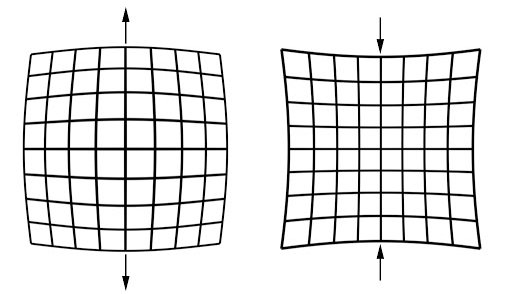
\includegraphics[width=0.68\textwidth]{figures/radial_distortion.jpg} 
	\caption{Radiálne skreslenie spôsobené zakrivením šošovky}
	\label{fig:radial_distortion}
\end{figure}

Neskreslené pixely označené $x$, $y$ sa nachádzajú v normalizovaných súradniciach obrázka. Normalizované súradnice sú vypočítané zo súradníc pixelov preložením do optického stredu a prepočítané pomocou ohniskovej vzdialenosti v pixeloch. Takže $x$ a $y$ sú bezrozmerné.

\begin{equation}
\label{eq::radial_dist::a}
\begin{aligned}
x'= x \frac{1 + k_{1}r^{2} + k_{2}r^{4} + k_{3}r^{6}}{1 + k_{4}r^{2} + k_{5}r^{4} + k_{6}r^{6}}
\end{aligned}
\end{equation}

\begin{equation}
\label{eq::radial_dist::b}
\begin{aligned}
y'= y \frac{1 + k_{1}r^{2} + k_{2}r^{4} + k_{3}r^{6}}{1 + k_{4}r^{2} + k_{5}r^{4} + k_{6}r^{6}}
\end{aligned}
\end{equation}

\begin{equation}
\label{eq::radial_dist::c}
\begin{aligned}
r^2=x^2+y^2
\end{aligned}
\end{equation}

Ak je $k_1<0$ , tak je skreslenie súdkovité a ak $k_1> 0$, tak ide o skreslenie poduškovité. Koeficienty $k_3$ a vyššie sú pri bežných deformáciách zvyčajne rovné 0. Prejavujú sa prevažne pri širokouhlých objektívoch. $r$ reprezentuje rádius k hlavnému bodu, kde nie je skreslenie.  

\subsection{Tangenciálne skreslenie}

Tangenciálne skreslenie vzniká pri neparalelnom umiestnení senzora kamery so šošovkou. Koeficienty $p_1$ a $p_2$ predstavujú tangenciálne skreslenie šošovky:

\begin{figure}[h]
	\centering
	%	\url{https://www.researchgate.net/figure/Tangential-distortion_fig5_332199146}
	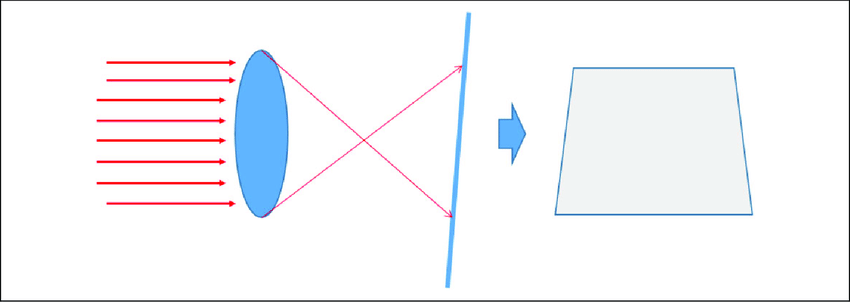
\includegraphics[width=0.7\textwidth]{figures/tangential_distortion.png} 
	\caption{Tangenciálne skreslenie spôsobené nesprávnym umiestnením šošovky}
	\label{fig:tangential_distortion}
\end{figure}

\begin{equation}
\label{eq::tangential_dist::a}
\begin{aligned}
x'= 2p_{1}xy + p_{2}\left(r^{2} + 2x^{2}\right)
\end{aligned}
\end{equation}

\begin{equation}
\label{eq::tangential_dist::b}
\begin{aligned}
y'= p_{1}\left(r^{2} + 2x^{2}\right) + 2p_{2}xy
\end{aligned}
\end{equation}

\begin{equation}
\label{eq::tangential_dist::c}
\begin{aligned}
r^2=x^2+y^2
\end{aligned}
\end{equation}

\subsection{Model reálnej kamery s korekciou skreslenia šošoviek}

V reálnych podmienkach je model ideálnej (dutinkovej) kamery doplnený o rovnice korekcie skreslenia šošoviek (tangenciálneho a radiálneho). Potreba získania koeficientov kamery je veľmi dôležitá z hľadiska správnej spätnej rekonštrukcie 2D obrazu do 3D priestoru.

\begin{equation}
\label{eq::real_camera::a}
\begin{aligned}
\begin{bmatrix}
u \\ v \\ z
\end{bmatrix} = R
\begin{bmatrix}
X \\ Y \\ Z
\end{bmatrix} + t 
\end{aligned}
\end{equation}

\begin{equation}
\label{eq::real_camera::b}
\begin{aligned}
x'= \frac{x}{z}; y'= \frac{y}{z}
\end{aligned}
\end{equation}

\begin{equation}
\label{eq::real_camera::d}
\begin{aligned}
x''= x' \frac{1 + k_{1}r^{2} + k_{2}r^{4} + k_{3}r^{6}}{1 + k_{4}r^{2} + k_{5}r^{4} + k_{6}r^{6}} + 2p_{1}x'y' + p_{2}\left(r^{2} + 2x'^{2}\right)
\end{aligned}
\end{equation}

\begin{equation}
\label{eq::real_camera::e}
\begin{aligned}
y''= y' \frac{1 + k_{1}r^{2} + k_{2}r^{4} + k_{3}r^{6}}{1 + k_{4}r^{2} + k_{5}r^{4} + k_{6}r^{6}} + p_{1}\left(r^{2} + 2y'^{2}\right) + 2p_{2}x'y'
\end{aligned}
\end{equation}


\begin{equation}
\label{eq::tangential_dist::f}
\begin{aligned}
u = f_{x} x'' + c_{x}; v = f_{y} y'' + c_{y}
\end{aligned}
\end{equation}


\section{Kalibrácia}

Kalibrácia kamery je nevyhnutný krok v 3D spracovaní obrazu, kde sa získavajú metrické informácie z 2D obrazov. Kalibráciu môžeme rozdeliť na 3 základné kategórie.

\textbf{Kalibrácia pomocou korešpondencie bodov v 3D priestore}\newline
Kalibrácia kamery sa vykonáva pozorovaním kalibračného objektu, ktorého geometria v 3D priestore je známa s veľmi presnou presnosťou. Kalibráciu je možné vykonať veľmi efektívne. Kalibračný objekt sa obvykle skladá z dvoch alebo troch rovín kolmých na seba.
%O. Faugeras,Three-Dimensional Computer Vision: A Geometric Viewpoint.MITPress, 1993.

\textbf{Autokalibrácia} 

Táto technika nepoužíva žiadny kalibračný objekt. Posunutím kamery v statickej scéne je možné vypočítať vnútorné parametre kamier. Ak sú snímky zosnímané tou istou kamerou s pevnými vnútornými parametrami, korešpondencia medzi tromi obrázkami je dostatočná na vypočítanie interných aj externých parametrov, ktoré nám umožňujú rekonštruovať 3D štruktúru. 

\textbf{Kalibrácia pomocou 2D roviny v 3D priestore}




Parametre kamery sa skladajú z vnútorných (intrinsických), vonkajších (extrinsických) koeficientov a koeficientov skreslenia (distortion). K určeniu je potrebné mať 3D body scény (world points) a ich zodpovedajúce 2D body. Získanie týchto korešpondujúcích dát je možné extrakciou ľahko identifikovateľných bodov. Jedným z najpoužívanejších kalibračných vzorov je šachovnica, kde je výrazný farebný prechod medzi hracími poľami (8).



%\section{Planárna homografia}
%Ide o lineárnu perspektívnu transformáciu, ktorá prevádza pixel z jednej roviny $X$ do druhej $X'$ v projektívnom priestore. 
%Homografia je využiteľná 3 spôsobmi:
%
%\begin{description}[leftmargin=*,labelsep=5.8mm, font=$\bullet$~\normalfont\scshape\color{black}]
%	\item Prevod roviny v 3D svetových súradniciach do 2D priestoru obrazovej roviny
%	\item Projektová transformácia, zobrazenie 3D plochy dvoma kamerami
%\end{description}
%
%\begin{equation}
%\label{eq_planar}
%\begin{aligned}
%X'=H \cdot X =
%\begin{bmatrix}
%x' \\ y' \\ 1 
%\end{bmatrix}
%= H
%\begin{bmatrix}
%x \\ y \\ 1 
%\end{bmatrix} =
%\begin{bmatrix}
%h_{11} & h_{12} & h_{13}  \\
%h_{21} & h_{22} & h_{23}  \\
%h_{31} & h_{32} & h_{33}  \\
%\end{bmatrix}
%\begin{bmatrix}
%x \\ y \\ 1 
%\end{bmatrix}
%\end{aligned}
%\end{equation}
%
%$H$ je  matica  rozmeru  3x3  a  má  8  nezávislých  parametrov.  Minimálny  počet štyroch  bodov zodpovedajúcich párov (N=4) je potrebných na zabezpečenie riešenia v rámci dovoleného rozsahu. Na spoľahlivé riešenie je potrebné mať viac ako 4 páry.
%
%
%
%Z kalibrácie je možné získať informácie o:
%
%\begin{description}[leftmargin=*,labelsep=5.8mm, font=$\bullet$~\normalfont\scshape\color{black}]
%	\item relatívnej polohe fotoaparátu a snímaného objektu 
%	\item chybe reprojekcie 3D objektu v 2D rovine 
%	\item chybe estimácie parametrov
%\end{description}
%
%Ku kalibrácií sa používa model štrbinovej kamery (pinhole camera model) a skreslenie šošoviek. Model štrbinovej kamery nezohľadňuje skreslenie šošoviek, pretože ideálna kamera nemá objektív (21)
%
%


	\chapter{Tézy dizertačnej práce}
\label{kap:tezy}
\pagestyle{fancy}
\fancyhf{}
\fancyfoot[CE,CO]{\thepage}
\renewcommand{\footrulewidth}{1pt}
\lhead{Tézy dizertačnej práce}



\begin{itemize}
	\item Návrh algoritmu umožňujúceho vytvorenie precízneho priestorového modelu objektu z viacerých kamier vrátane kalibrácie vizuálneho systému.
	\item Návrh algoritmu pre automatizovanú detekciu kľúčových bodov na objekte a automatizované meranie vybraných geometrických priestorových parametrov.
\end{itemize}



Riešenie úlohy definovanej v prvej fáze je založené na využití multi-kamerového systému, ktorý v reálnom čase dokáže zachytiť priestorovú informáciu snímanej scény. Jednotlivé priestorové informácie z kamier sa následne zlúčia do spoločného priestorového modelu, ktorý bude použitý pre riešenie druhej tézy.
Podstatnou problematikou je vzájomná kalibrácia multi-kamerového systému a návrh filtračného algoritmu, ktorým sa zvýši kvalita výstupných priestorových dát. 

Problematika druhej tézy môže byť riešená viacerými spôsobmi. Podstatným krokom je identifikácia kľúčových bodov alebo oblastí v priestorovom modely. Jedným z možných riešení je segmentácia RGB-D mapy, kde sa pomocou algoritmov klasifikujú regióny bodov. Z výsledku klasifikácie bude následne možné rekonštruovať iba vybrané regióny 3D priestorového modelu. Výsledkom bude množina mračien bodov, ktoré môžu vystupovať ako samostatné modely alebo budú reprezentovať ucelený konzistentný model.




	
\chapter{Návrh systému} 
\label{kap:návrh systému}
\pagestyle{fancy}
\fancyhf{}
\fancyfoot[CE,CO]{\thepage}
\renewcommand{\footrulewidth}{1pt}
\lhead{Návrh systému}


\section{Výber kamier}

\subsection{Intel Realsense SR300}

Táto kamera pracuje na princípe SLS a predstavuje vylepšenú verziu staršej Intel RealSense F200. Ide o cenovo dostupnú hĺbkovú kameru, ktorá sníma hĺbku v rozsahu od $0.2-1.5 m$. Poskytuje dynamické snímanie scény pri nízkej spotrebe (napájanie cez USB). V kombinácií s farebným obrazom ($1920\times1080p$, $30Hz$) a hĺbkovou mapou ($640x480p$) ide o jednu z najlepších dostupných SLS kamier na trhu. 

\begin{figure}[H]
	\centering
	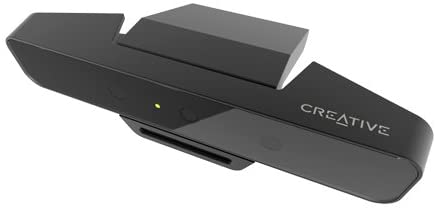
\includegraphics[width=0.7\textwidth]{figures/sr300.jpg}
	\caption{SLS kamera Intel RealSense SR300.}
	\label{fig::sr300}
\end{figure}

Táto kamera obsahuje RGB senzor, IR laserový projektor, IR prijímač a mikrofón. Detailnejšie opísanie princípu SLS je v podkapitole \ref{sec:sls}.

\subsection{Microsoft Kinect v2}

Ide o druhú generáciu hĺbkových kamier od spoločnosti Microsoft. Oproti prvej generácií využíva technológiu ToF (detailnejšie v \ref{sec:tof}), pričom ide o jednu z najznámejších senzorov tohto typu na svete. Rozsah snímanej scény je $0.5-4.5 m$. Farebný obraz je dodávaný v rozlíšení $1920\times1080p$ a $30Hz$, hĺbková mapa ma rozlíšenie $512\times424$.

\begin{figure}[H]
	\centering
	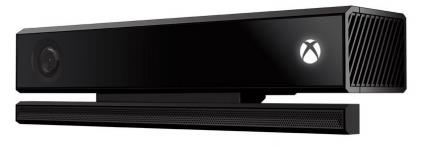
\includegraphics[width=0.7\textwidth]{figures/kinect.png}
	\caption{ToF kamera Microsoft Kinect v2.}
	\label{fig::kinect}
\end{figure}

Presnosť hĺbkovej mapy je oproti prvej verzii Kinectu vyššia, taktiež je znížený negatívny vplyv spôsobovaný slnečným svetlom.


\subsection{Porovnanie presnosti kamier}

Cieľom testovania bolo porovnať presnosť 3D rekonštrukcie statického objektu pre kamery Intel RealSense SR300 a Microsoft Kinect v2. Pomocou programov, určených k práci s jednotlivými kamerami, bola vytvorená séria snímok hĺbkových máp a ich rekonštruovaných 3D modelov. Pred snímaním bola vykonaná geometrická kalibrácia kamier, ktorej technické detaily sú opísané v kapitole \ref{sec:kinect_calib}. Kalibrovanými kamerami sa následne z 3 uhlov (pohľady spredu, z ľavej a pravej strany) získali ich 3D rekonštrukcie, ktoré zachytávali všetky potrebné detaily pre meranie. Identické natočenie pre obe kamery bolo zabezpečené rotačným podstavcom. 

\begin{figure}[H]
	\centering
	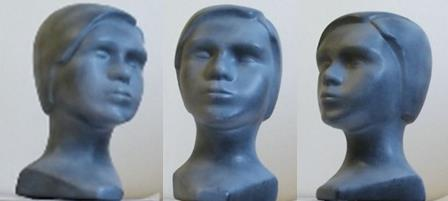
\includegraphics[width=0.7\textwidth]{figures/rgb_compar.png}
	\caption{ToF kamera Microsoft Kinect v2.}
	\label{fig::rgb_compare}
\end{figure}

Povrch objektu bol špeciálne upravený, aby nevytváral odlesky spôsobujúce zhoršovanie rekonštruovaného 3D modelu. 

\section{Snímanie dynamických objektov}

Pri snímaní dynamických objektov je potrebné uvažovať so vznikom pohybových artefaktov. Tie vznikajú, ak objekt v dobe skenovania mení svoje priestorové umiestnenie. Z toho dôvodu je potrebné buď stabilizovať objekt počas doby snímania alebo redukovať časovú dĺžku skenovania. Keďže tento systém má byť určený pre medicínske aplikácie, kde skenovaný objekt bude pediatrický pacient, je potrebné overiť možnosti experimentálne.


\subsection{Jedno-kamerové snímanie dynamických objektov}

Experimentálne snímanie pacientov bolo vykonávané na Klinike detí a dorastu Jesseniovej lekárskej fakulty v Martine, Laboratórium spánkovej medicíny. Do testu bolo vybraných 9 pacientov rôzneho pohlavia,vo vekovom rozmedzí od 4 do 12 rokov. 

Ako skenovací nástroj bola použitá kamera Kinect v2. V spolupráci s komerčným softvérom KScan3D boli vytvorené modely pacientov, ktoré sú zobrazené na obr. \ref{fig:dynamic_patient:a} a \ref{fig:dynamic_patient:b}. 

\begin{figure}[H]
	\centering
	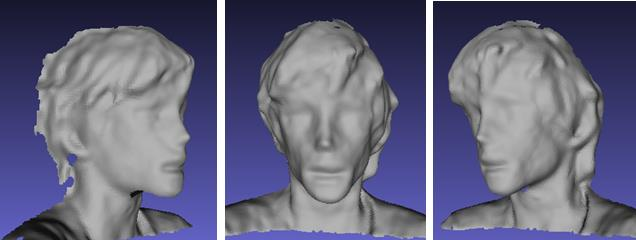
\includegraphics[width=\textwidth]{figures/dynamic_patient_a.png}
	\caption{ToF kamera Microsoft Kinect v2.}
	\label{fig:dynamic_patient:a}
\end{figure}

\begin{figure}[H]
	\centering
	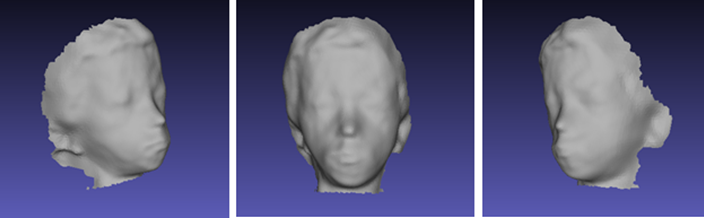
\includegraphics[width=\textwidth]{figures/dynamic_patient_b.png}
	\caption{Úkažka .}
	\label{fig:dynamic_patient:b}
\end{figure}

Ako je vidieť, modely sú nekvalitné a výrazne deformované. Je to spôsobené tým, že objekty nedokázali zostať v statickej polohe počas doby skenovania (tá presahovala 1 minútu pri každom pacientovi). Tendenciou bolo otáčať sa za kamerou, čo viac krát viedlo k nutnosti začas celý proces od znova. 

Takéto modely nie su postačujúce pre diagnostikovanie OSAS. Ich miera nepresnosti je veľmi vysoká a užitočná geometria tváre sa stráca. Z experimentu vyplýva, že jedno-kamerový systém je nepoužiteľný pre skenovanie dynamických objektov ako sú pediatrickí pacienti.  

\subsection{Priestorové rozloženie multi-kamerového systému}

Pri multi-kamerovom systéme sa pre skenovanie používajú viaceré kamery, ktoré su staticky rozložene v priestore. Ich počet závisí od detailov objektu, ktoré majú byť zosnímané.

\begin{figure}[H]
	\centering
	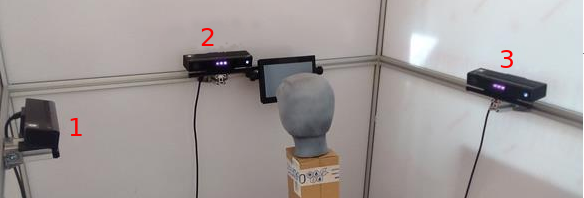
\includegraphics[width=0.6\textwidth]{figures/multicam_placement.png}
	\caption{Úkažka .}
	\label{fig:multicam:placement}
\end{figure}


Medzi hlavné požiadavky na model sú: hlava musí obsahovať laterálne pohľady (umožniť prekrytie s cefalometrickou snímkou) a orientačné bodov mäkkého tkaniva. Dôležité je aj získanie informácie o šírke krk. Na obrázku \ref{fig:multicam:placement} je zobrazené rozloženie kamier v skenovacej kabíne. Ich jednotlivé 3D modely aj s verifikáciou požiadaviek sa nachádzajú na obr. \ref{fig:multicam:models}. 

\begin{figure}[H]
	\centering
	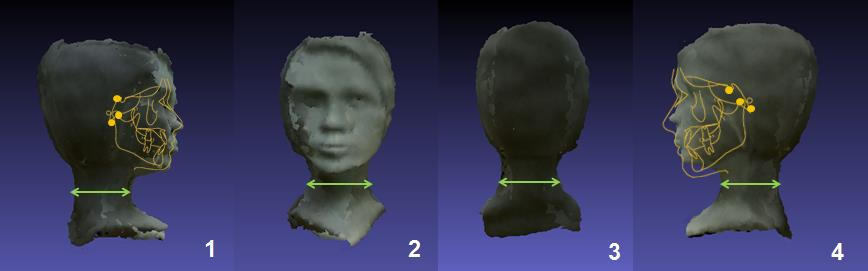
\includegraphics[width=\textwidth]{figures/multicam_placement_scans.png}
	\caption{Úkažka .}
	\label{fig:multicam:models}
\end{figure}

\subsection{Sekvenčné snímanie multi-kamerového systému}

Sekvenčný mód predstavuje postupné snímanie. V jednom momente vždy sníma len jedna kamera ostatné kamery sú vypnuté. Tento režim je pri ToF kamerách často využívaný, pretože tu nevzniká multi-kamerová interferencia. Problémom je však dlhá doba zapínania IR projektora, ktorá pri kamerách Microsoft Kinect v2 dosahuje približne $1s$. Časový odstup medzi dvoma prijatými snímkami je pri $30Hz$ okolo $33ms$.

\subsection{Paralelné snímanie multi-kamerového systému}

V paralelnom režime pracujú všetky kamery v rovnakom čase. Oproti sekvenčnému snímaniu sa inicializácia vykonáva pre každú kameru iba raz. Tým sa radikálne znižuje doba snímania objektu zo všetkých uhlov. Nevýhodou je ale vznik multi-kamerovej interferencie, ktorá dokáže negatívne ovplyvniť výstupné hĺbkové mapy. Časový rozostup medzi jednotlivými snímkami je ovplyvnení samotným spracovaním dát, maximálne však $33ms$ medzi všetkými snímkami. 

\subsection{Porovnanie režimov snímania dynamických objektov}

Pre porovnanie týchto režimov bol navrhnutý experiment, pri ktorom sa porovná veľkosť zmeny polohy objektu v závislosti na dĺžke snímania. Pre testovanie bol vyrobený merací prvok, ktorý pozostával z jednosmerného motora, ukazovateľa aktuálnej polohy a statického podstavca slúžiaceho ako uhlomer. Na hriadeli motora bol pripevnený ukazovateľ, ktorý vykonával pohyb po kružnici. Rýchlosť bola nastavená na regulovateľným zdrojom tak, aby otočka trvala $5s$. Obvod statického podstavca bol rozdelený na 36 dielov oddelených od seba po $10^\circ$. Kvôli identifikácii polohy podstavec obsahoval zvýraznený nultý bod a šípku informujúcu o smere otáčania ukazovateľa.  

\begin{figure}[h]
	\centering
	\begin{subfigure}[b]{\textwidth}
		\centering
		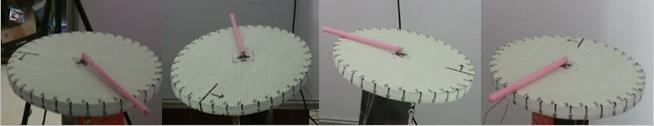
\includegraphics[width=\textwidth]{figures/dynamic_sequence.png}
		\label{fig:dynamic:sequence}
	\end{subfigure}
	\vfill
	\begin{subfigure}[b]{\textwidth}
		\centering
		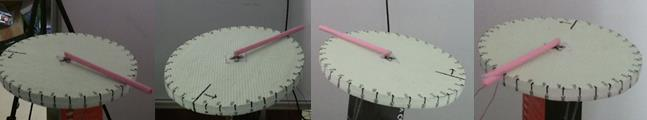
\includegraphics[width=\textwidth]{figures/dynamic_parallel.png}
		\label{fig:dynamic:parallel}
	\end{subfigure}
	\caption{}
	\label{fig:dynamic:results}
\end{figure}

Pri sekvenčnom režime boli snímky z kamier získavané postupne od 1 po 4 kameru. Pri paralelnom režime je ťažké identifikovať poradie. Pre porovnanie bolo potrebné získané hĺbkové mapy previesť na mračno bodov a pomocou ICP metódy ich registrovať do jedného modelu (zhodná pozícia nultého bodu). 

\begin{figure}[h]
	\centering
	\begin{subfigure}[b]{0.42\textwidth}
		\centering
		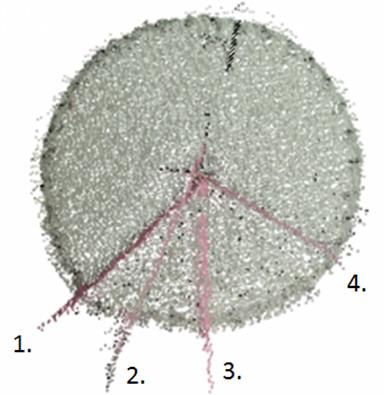
\includegraphics[width=\textwidth]{figures/dynamic_result_seq.png}
		\caption{}
		\label{fig:depthir:a}
	\end{subfigure}
	\hfill
	\begin{subfigure}[b]{0.42\textwidth}
		\centering
		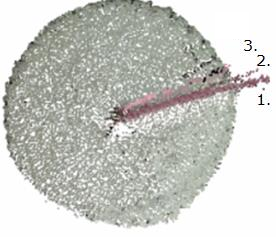
\includegraphics[width=\textwidth]{figures/dynamic_result_par.png}
		\caption{}
		\label{fig:depthir:b}
	\end{subfigure}
	\caption{Obrazy z senzora Microsoft Kinect v2: (\textbf{a}) IR obraz bez interferencie. (\textbf{b}) IR obraz s interferenciou. (\textbf{c}) Hĺbková mapa IR obrazu (a). (\textbf{d}) Hĺbková mapa IR obrazu (b). Miesto interferencie je zvýraznené červenou farbou.}
	\label{fig:depthir}
\end{figure}

Z výsledných modelov je jasne vidieť, že paralelné spracovanie dát má vyšší zmysel pri snímaní dynamických objektov. Pri sekvenčnom režime je rozdiel polohy ukazovateľa výrazný, čo spôsobovalo problémy aj pri ICP registrácií. Naproti tomu je model vytvorený paralelným režimom konzistentnejší, rozdiel polohy ukazovateľa je podstatne menší. Ten by sa dal znížiť hardvérovým synchronizovaným snímaním. Pri kamerách Kinect v2 však táto možnosť chýba.

\section{Kalibrácia kamier systému}
\label{sec:kinect_calib}
Pre kalibráciu bol použitý \textit{Matlab Calibration ToolBox}. 

\subsection{Geometricka kalibrácia}
Cieľom geometrickej kalibrácie je získanie vnútorných parametrov  kamery spolu s korekčnými parametrami pre odstránenie tangenciálneho a radiálneho skreslenia. Tieto parametre bolo potrebne získať pre RGB aj IR senzory všetkých používaných hĺbkových kamier Kinect v2. 

Pre kalibráciu RGB a IR senzora sa vytvorila séria snímok, ktoré  obsahovali kalibračný vzor snímaný z rôznych uhlov. Ten bol reprezentovaný šachovnicovým motívom o rozmeroch $10\times8$, pričom dĺžka hrany mala veľkosť $36mm$.


%\begin{figure}[h]
%	\centering
%	\begin{subfigure}[b]{0.59\textwidth}
%		\centering
%		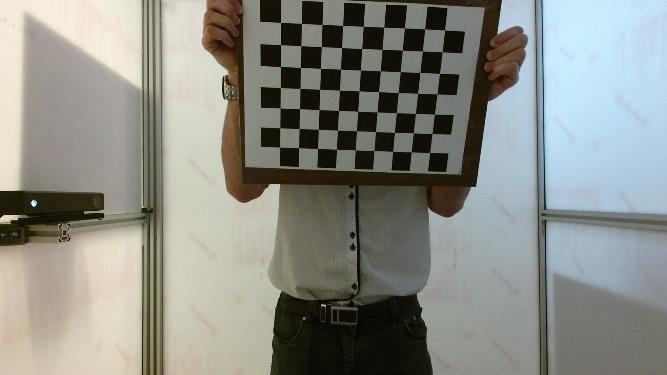
\includegraphics[width=\textwidth]{figures/calibration_rgb.png}
%		\caption{}
%		\label{fig:calib:rgb}
%	\end{subfigure}
%	\hfill
%	\begin{subfigure}[b]{0.4\textwidth}
%		\centering
%		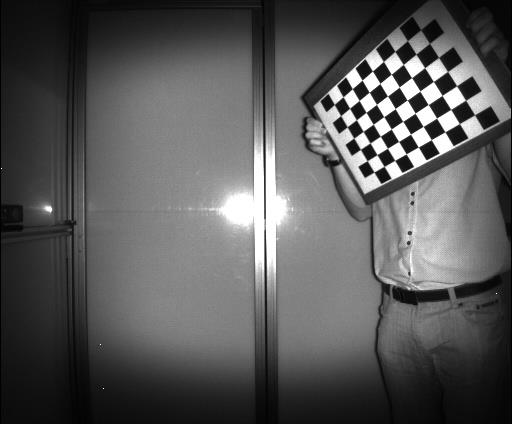
\includegraphics[width=\textwidth]{figures/calibration_ir.png}
%		\caption{}
%		\label{fig:calib:ir}
%	\end{subfigure}
%	\caption{Obrazy z senzora Microsoft Kinect v2: (\textbf{a}) IR obraz bez interferencie. (\textbf{b}) IR obraz s interferenciou. (\textbf{c}) Hĺbková mapa IR obrazu (a). (\textbf{d}) Hĺbková mapa IR obrazu (b). Miesto interferencie je zvýraznené červenou farbou.}
%	\label{fig:calib:single}
%\end{figure}

Pre overenie správnosti kalibrácie IR snímača sa porovnával kalibrovaný kamerový systém s nekalibrovaným voči referenčnému modelu. Pri rovnakých podmienkach prostredia bol zosnímaný model hlavy s továrenskými nastaveniami, potom boli použité kalibračné koeficienty získané v predchádzajúcom kroku. Referenčný model bol vytvorený ručným laserovým skenerom. Ukážky sa nachádzajú na obr. \ref{fig:calib:models}. 

\begin{figure}[H]
	\centering
	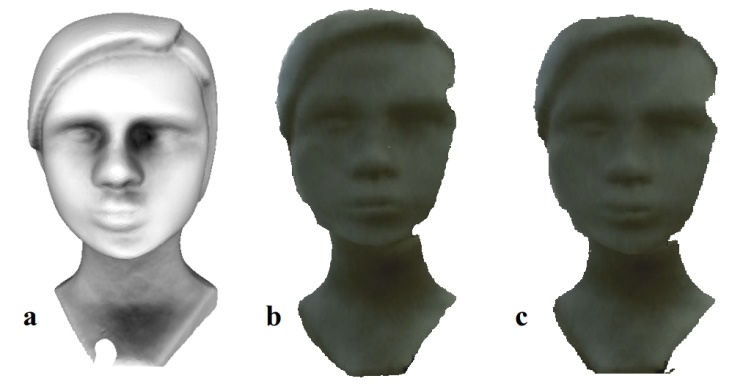
\includegraphics[width=0.6\textwidth]{figures/calibration_models.jpg}
	\caption{}
	\label{fig:calib:models}
\end{figure}

Porovnanie priestorovej rekonštrukcie hĺbkových máp bolo robené pomocou Hausdorffovej vzdialenosti. V nej je detailnejšie zobrazené, aký vplyv má kalibrácia na generované dáta. Z modelu vzdialenosti (obr. \ref{fig:calib:haus:single}) je vidieť, že nekalibrovaný systém vykazoval vyššiu chybu na okrajoch modelu. To je spôsobené pozitívnym radiálnym skreslením IR senzora, ktorého intenzita je výraznejšia na okrajoch obrazu. Štatistické výsledky pre 10 modelov sa nachádzajú v tabuľke \ref{tab:calib:single}.

\begin{figure}[H]
	\centering
	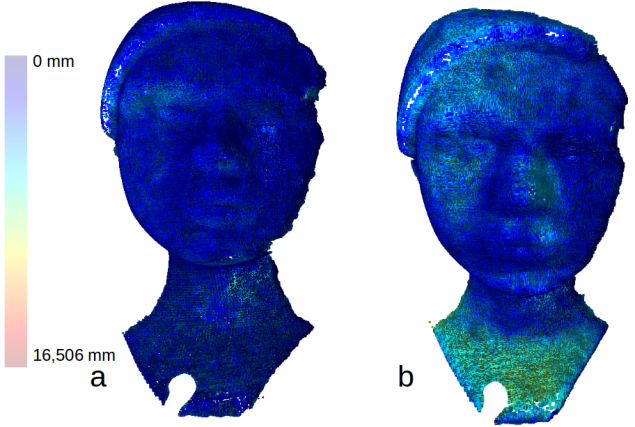
\includegraphics[width=0.52\textwidth]{figures/calibration_hausdorff_single.jpg}
	\caption{}
	\label{fig:calib:haus:single}
\end{figure}



\begin{table}[h]
	\caption{\label{tab:calib:single} Štatistické porovnanie geometrickej kalibrácie kamier }
	\centering
	\begin{tabular}{cccc}
		\toprule
		\textbf{Model} & \textbf{Počet bodov [-]} & \textbf{Mean [mm]} & \textbf{RMS [mm]} \\ 
		\midrule
		\textbf{Nekalibrovaný} & 185187 & 3,0206	& 3,8444 \\
		\textbf{Kalibrovaný} & 296585   & 2,1832   & 2,9506  \\  
		\bottomrule
	\end{tabular}
\end{table}

Týmto krokom sa overil spôsob geometrickej kalibrácie hĺbkových máp. V systéme, kde sa využíva viacero kamier a je kladený dôraz na precíznosť rekonštrukcie, ide o nevyhnutný krok. 


\subsection{Multi-kamerová kalibrácia}

V tomto procese sa hľadajú vzájomné pozície kamier vo svetovej súradnicovej sústave. Ich vzájomnú pozíciu určujú rotačné a translačné parametre (kombinácia afinných transformácií z kapitoly \ref{sec:afine}). Tie je možné získať viacerými spôsobmi. Dôležité je si určiť referenčnú kameru, ktorej matica vonkajších parametrov bude mať tvar identickej afinnej transformácie. Pri multi-kamerovej kalibrácií sa využíva podobný postup ako pri geometrickej kalibrácii. Rozdielom je však, že sa kalibračný vzor sníma súčasne z viacerých kamier. Problém nastáva, ak ich rozloženie neumožňuje súčasné snímanie. Takýto prípad je zachytený na obr. \ref{fig:multicam:placement}.

Riešením je separátne kalibrovanie medzi susednými kamerami (napr. 1-2, 1-3 a 2-4 alebo 3-4). 

\begin{figure}[H]
	\centering
	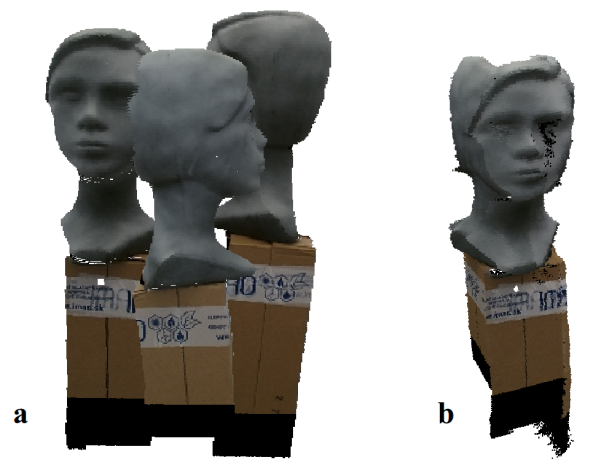
\includegraphics[width=0.52\textwidth]{figures/calibration_multi.jpg}
	\caption{}
	\label{fig:calib:haus:single}
\end{figure}

\begin{figure}[H]
	\centering
	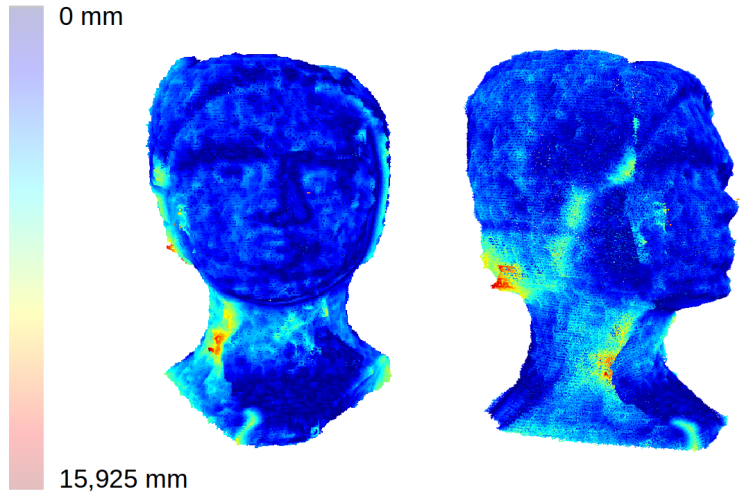
\includegraphics[width=0.52\textwidth]{figures/calibration_hausdorff_multi.jpg}
	\caption{}
	\label{fig:calib:haus:single}
\end{figure}


\begin{equation}
\label{eq:multi:calib:a}
\begin{aligned}
\begin{bmatrix}
1 & 0 & 0 & 0 \\
0 & 1 & 0 & 0 \\
0 & 0 & 1 & 0 \\
0 & 0 & 0 & 1 
\end{bmatrix}, 
\begin{bmatrix}
1 & -0.03 & 0.06 & -0.03 \\
0.02 & 1 & 0.07 & -0.04 \\
-0.06 & -0.06 & 1 & 0.02 \\
0 & 0 & 0 & 1 
\end{bmatrix}
\end{aligned}
\end{equation}




\section{Návrh algoritmu}


\subsection{Paralelné spracovanie dát}

\subsection{Analýza pohybu objektu}

\subsection{ICP registrácia}

\subsection{Segmentácia hĺbkovej mapy}

	\chapter{Potláčanie multi-kamerovej interferencie ToF senzorov} 
\label{kap:interference}
\pagestyle{fancy}
\fancyhf{}
\fancyfoot[CE,CO]{\thepage}
\renewcommand{\footrulewidth}{1pt}
\lhead{Potláčanie multi-kamerovej interferencie ToF senzorov}

Jedným z nevýhod použitia ToF senzorov je ich multi-kamerová interferencia (MCI). Ide o chybu, ktorá ma fyzikálnu podstatu a má veľmi negatívny dopad na výstupné dáta. Ak pri snímaní scény nastane táto interferencia, skenovací systém sa stáva nepoužiteľným. 

Jednou z možnosti riešenia problému je použitie kamier, ktoré pracujú na rozdielnych modulačných frekvenciách emitovaného svetla. Mnoho nedávnych prác zaoberajúcich sa problémom multi-kamerovej interferencie  uvádzajú, že ToF senzory sa nesmú prevádzkovať s rovnakou modulačnou frekvenciou \cite{Kim}. Spoliehajú sa na ortogonálne funkcie, ako sú sínusoidy s rôznou frekvenčnou moduláciou. Toto riešenie je však obmedzujúce, pretože vzniká problém softvérovej kompatibility s pripojením rôznych typov kamier v jednej aplikácii \cite{Buttgen, Whyte, Seitz}.
Pomocou metódy LSENS je možné obnoviť informácie o hĺbke a amplitúde. Táto metóda je založená na analýze štatistických vlastností interferencie signálu \cite{Lianhua}. Interferenčný signál však musí mať kladné a záporné pulzovanie hĺbkovej mapy. V situáciách, keď sú kamery namierené proti sebe, môže byť kolísanie signálu extrémne vysoké. V takom prípade nebude metóda LSENS účinná. Z analýzy výstupných dát je však možné určiť podmienky potlačenia interferencie a podľa nich navrhnúť filtračný algoritmus. Úlohou filtra je odstrániť čo najviac poškodených dát pri čo najmenšej strate relevantných dát.    


\section{Model ToF kamery}

ToF senzory sú optické snímače, ktoré poskytujú informácie o hĺbke scény. Obsahujú aktívny svetelný zdroj, ktorý generuje amplitúdovo modulovaný signál. Signál môže mať spojitý alebo impulzný charakter. Väčšina ToF kamier vyžaruje amplitúdovo modulovanú kontinuálnu vlnu (AMCW) s frekvenciou blízkou IR na osvetlenie scény. Meranie hĺbky je založené na meraní amplitúdy fázového posunu vysielaného a prijímaného modulovaného signálu (Obr. \ref{fig::tof}). Informácie o hĺbke pre každý pixel sa môžu vypočítať pomocou synchronného demodulovania prijatého modulovaného svetla v detektore. Demodulovanie sa môže uskutočniť preložením s pôvodným modulovaným signálom. Tento proces sa nazýva krížová korelácia. Všeobecne je korelačná funkcia definovaná rovnicou \ref{eq::tof::01}.

\begin{figure}[H]
	\centering
	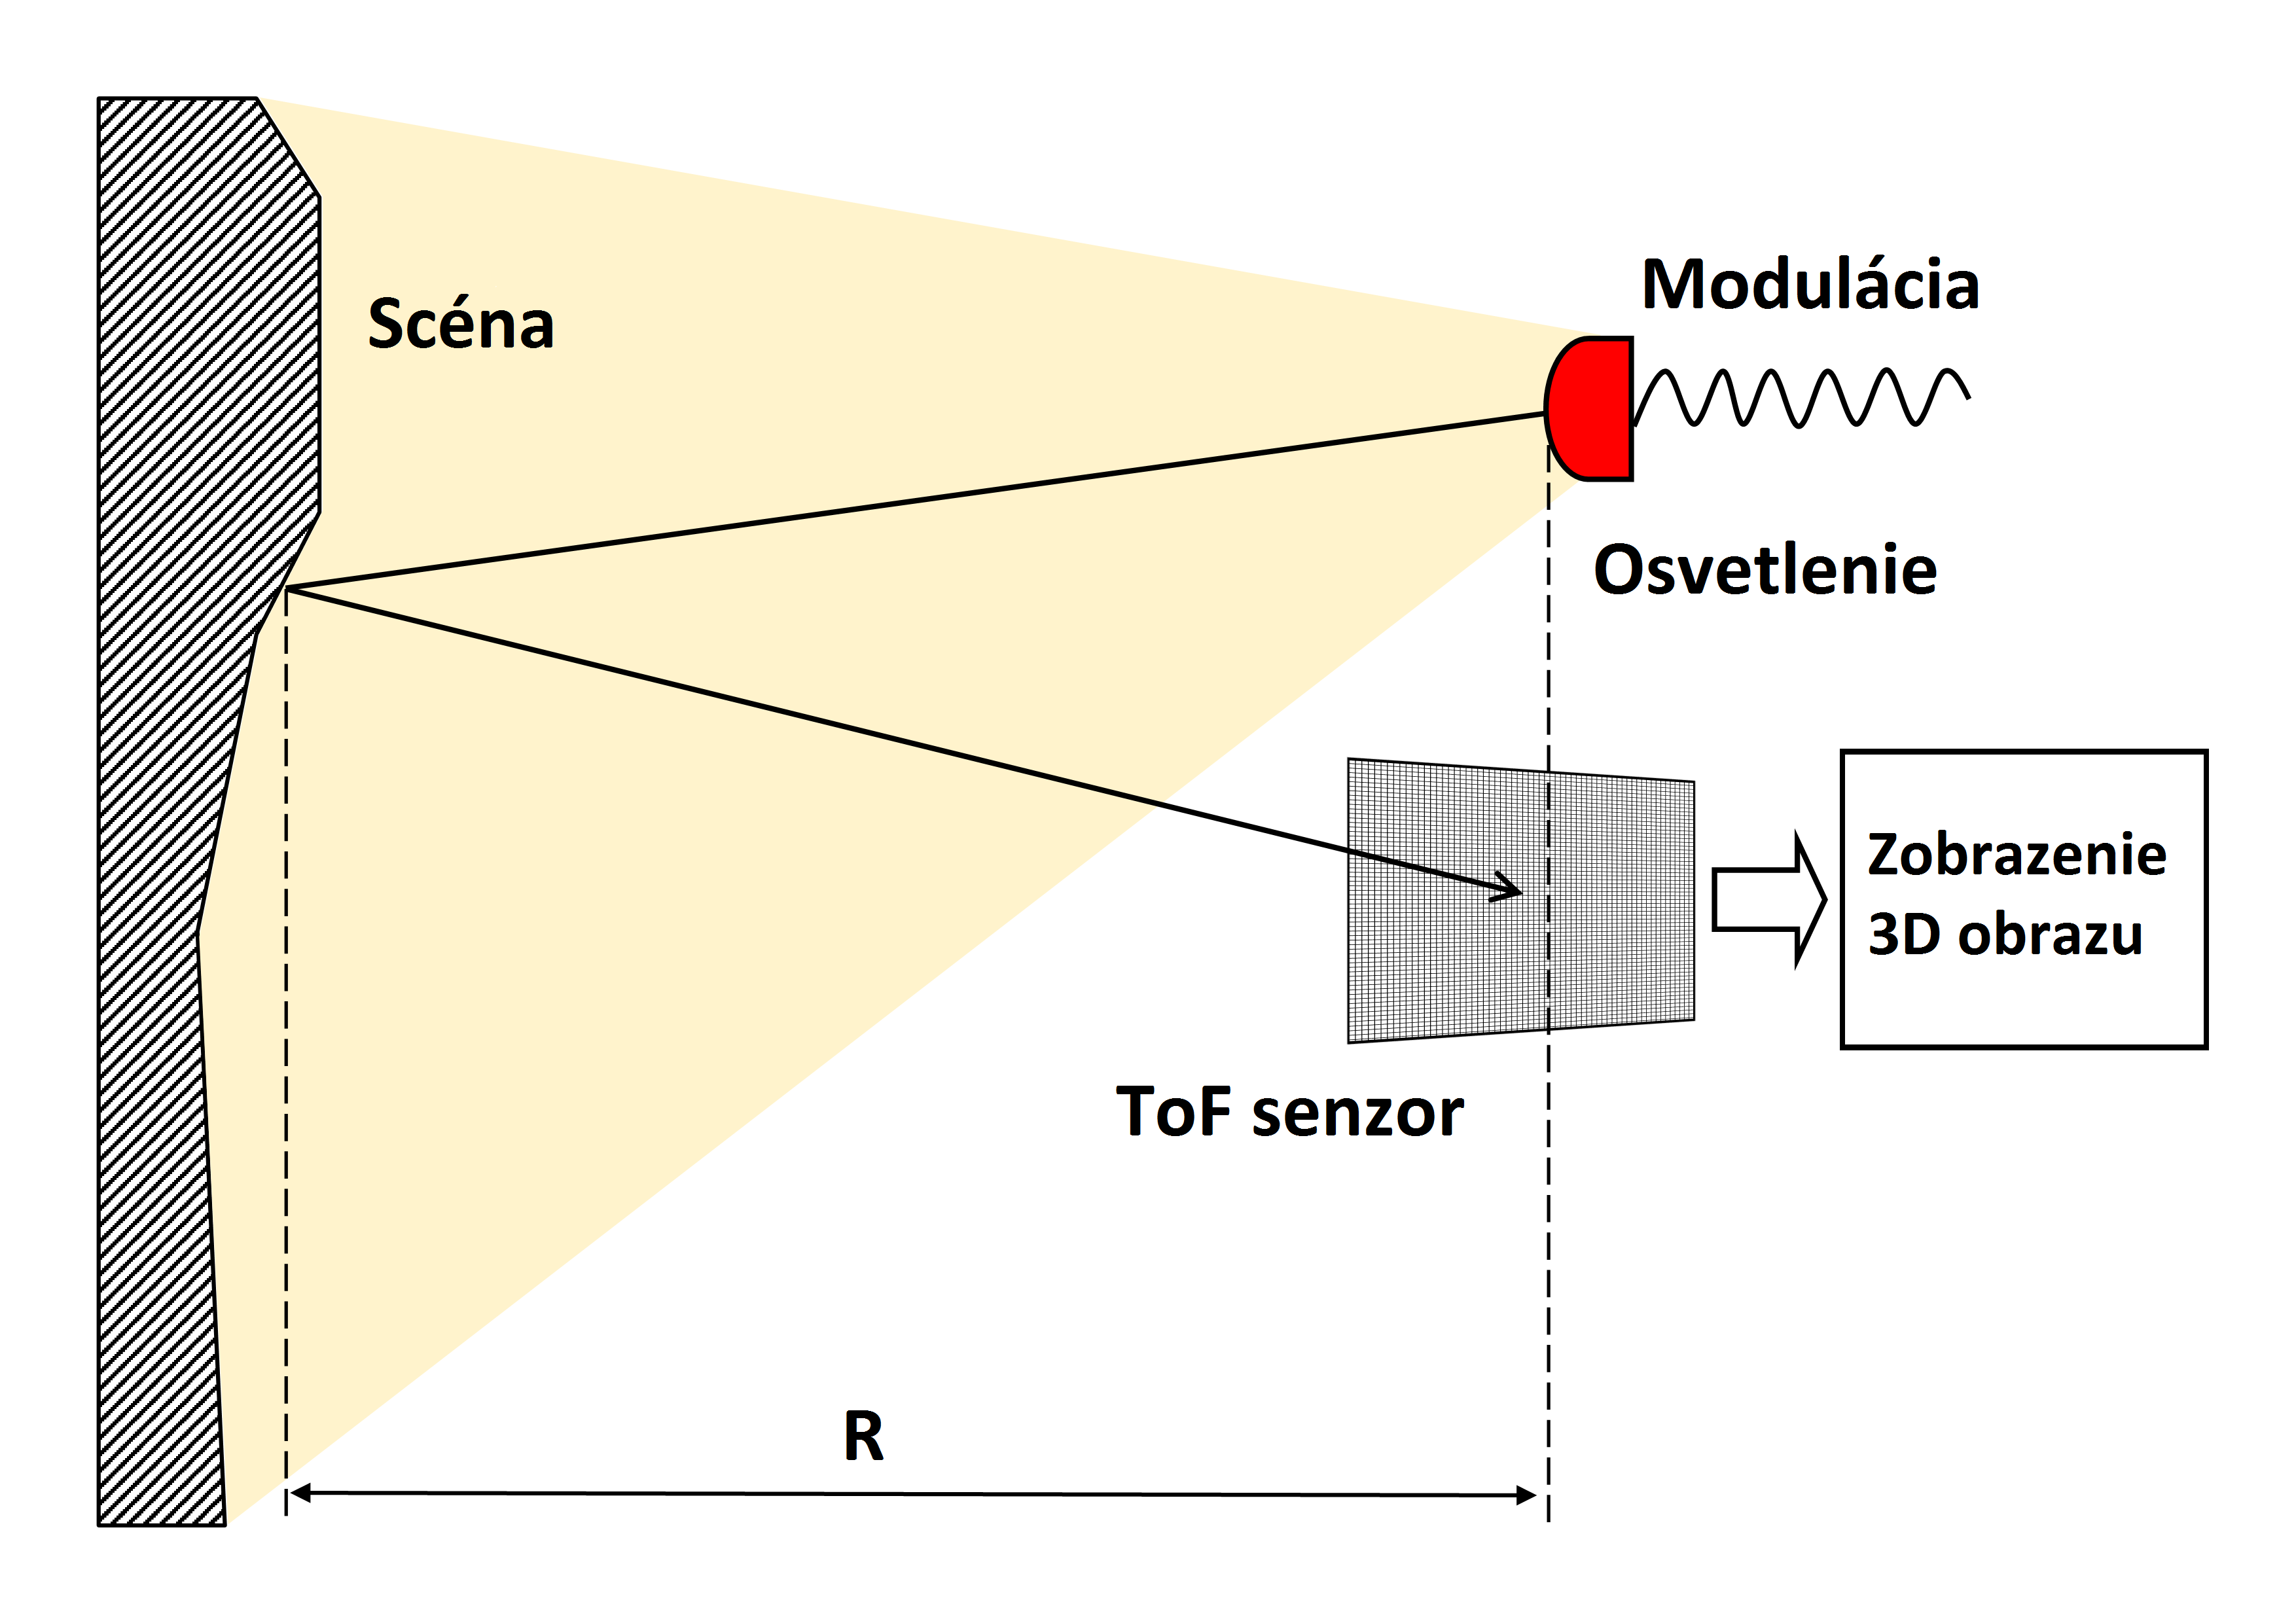
\includegraphics[width=0.65\textwidth]{figures/tof.png}
	\caption{Princíp činnosti merania fázového posunu pri ToF kamerách \cite{Lianhua}.}
	\label{fig::tof}
\end{figure}

\begin{equation}
\label{eq::tof::01}
c(\tau) = s(t) \otimes g(t) = \lim_{T \to \infty} {\frac{1}{T}} \int_{-\frac{T}{2}}^{\frac{T}{2}}{s(t) \cdot g(t+ \tau)}dt
\end{equation}


\noindent kde $s(t)$ je prijatý optický signál a $g(t)$ je vyžiarený (pôvodný) signál. Použitím špecifických funkcií pre kamery ToF dostaneme rovnice

\begin{equation}
\label{eq::tof::02}
g(t) = \cos{\omega t}
\end{equation}

\begin{equation}
\label{eq::tof::03}
s(t) = 1+a\cdot \cos{(\omega t - \varphi)}
\end{equation}

\begin{equation}
\label{eq::tof::04}
\begin{aligned}
c(\tau) = \varphi_{sg}(\tau) =  {{\frac{a}{2}} \cdot cos(\varphi + \omega \tau)}
\end{aligned}
\end{equation}

\noindent kde $a$ je amplitúda modulácie a $\varphi$ je fázový posun.
\noindent Táto funkcia je vypočítaná pre štyri rôzne $\omega t$ argumenty, ktoré sú posunuté z 0 o $\ang{90}$.
Prijatý signál je väčšinou navrstvený na pozadí obrazu, čo vyžaduje pridanie offsetu $ b $ do korelačnej funkcie:

\begin{equation}
\label{eq::tof::05}
\begin{aligned}
C(\tau) = c(\tau) + b
\end{aligned}
\end{equation}

\begin{equation}
\label{eq::tof::06}
\begin{aligned}
C(\tau _0) = c(\tau _0) + b}=  {{\frac{a}{2}} \cdot cos(\varphi) +b \\
C(\tau _1) = c(\tau _1) + b}= - {{\frac{a}{2}} \cdot sin(\varphi) +b \\
C(\tau _2) = c(\tau _2) + b}=- {{\frac{a}{2}} \cdot cos(\varphi) +b \\
C(\tau _3) = c(\tau _3) + b}= {{\frac{a}{2}} \cdot sin(\varphi) +b 
\end{aligned}
\end{equation}

\noindent S týmito štyrmi vybranými bodmi je možné vypočítať korelačnú funkciu a určiť fázu $\varphi$ a amplitúdu $a$ prijatého signálu $s(t)$:

\begin{equation}
\label{eq::tof::07}
\begin{aligned}
\varphi = atan \Bigg[ {\frac{C(\tau _3) - C(\tau _1)}{C(\tau _0) - C(\tau _2)}} \Bigg]
\end{aligned}
\end{equation}

\begin{equation}
\label{eq::tof::08}
\begin{aligned}
a =  \frac{\sqrt{{[C(\tau _3) - C(\tau _1)}]^2 + [{C(\tau _0) - C(\tau _2)}]^2}}{2}  
\end{aligned}
\end{equation}


\noindent Hĺbka $d$ sa vypočíta podľa nasledujúcej rovnice:


\begin{equation}
\label{eq::tof::09}
\begin{aligned}
d = \frac{ c \cdot \varphi }{ 2 \cdot 2 \pi f}
\end{aligned}
\end{equation}

\noindent kde $c$ je rýchlosť svetla a $f$ je frekvencia modulácie IR \cite {Lange}.


\section{Model multi-kamerovej interferencie}

V multi-kamerovom režime každý ToF senzor používa rovnakú modulačnú frekvenciu a IR vlnovú dĺžku, takže prijaté signály interagujú navzájom. V experimentálnej topológii senzorov používame tri ToF senzory S1 \, - \, S3, ktoré sú statické a umiestnené v skenovacej kabíne. Tento systém je znázornený na obrázku \ref{fig:imodel}, ktorý popisuje vzájomné vzťahy medzi jednotlivými kamerami a objektom.

\begin{figure}[H]
	\centering
	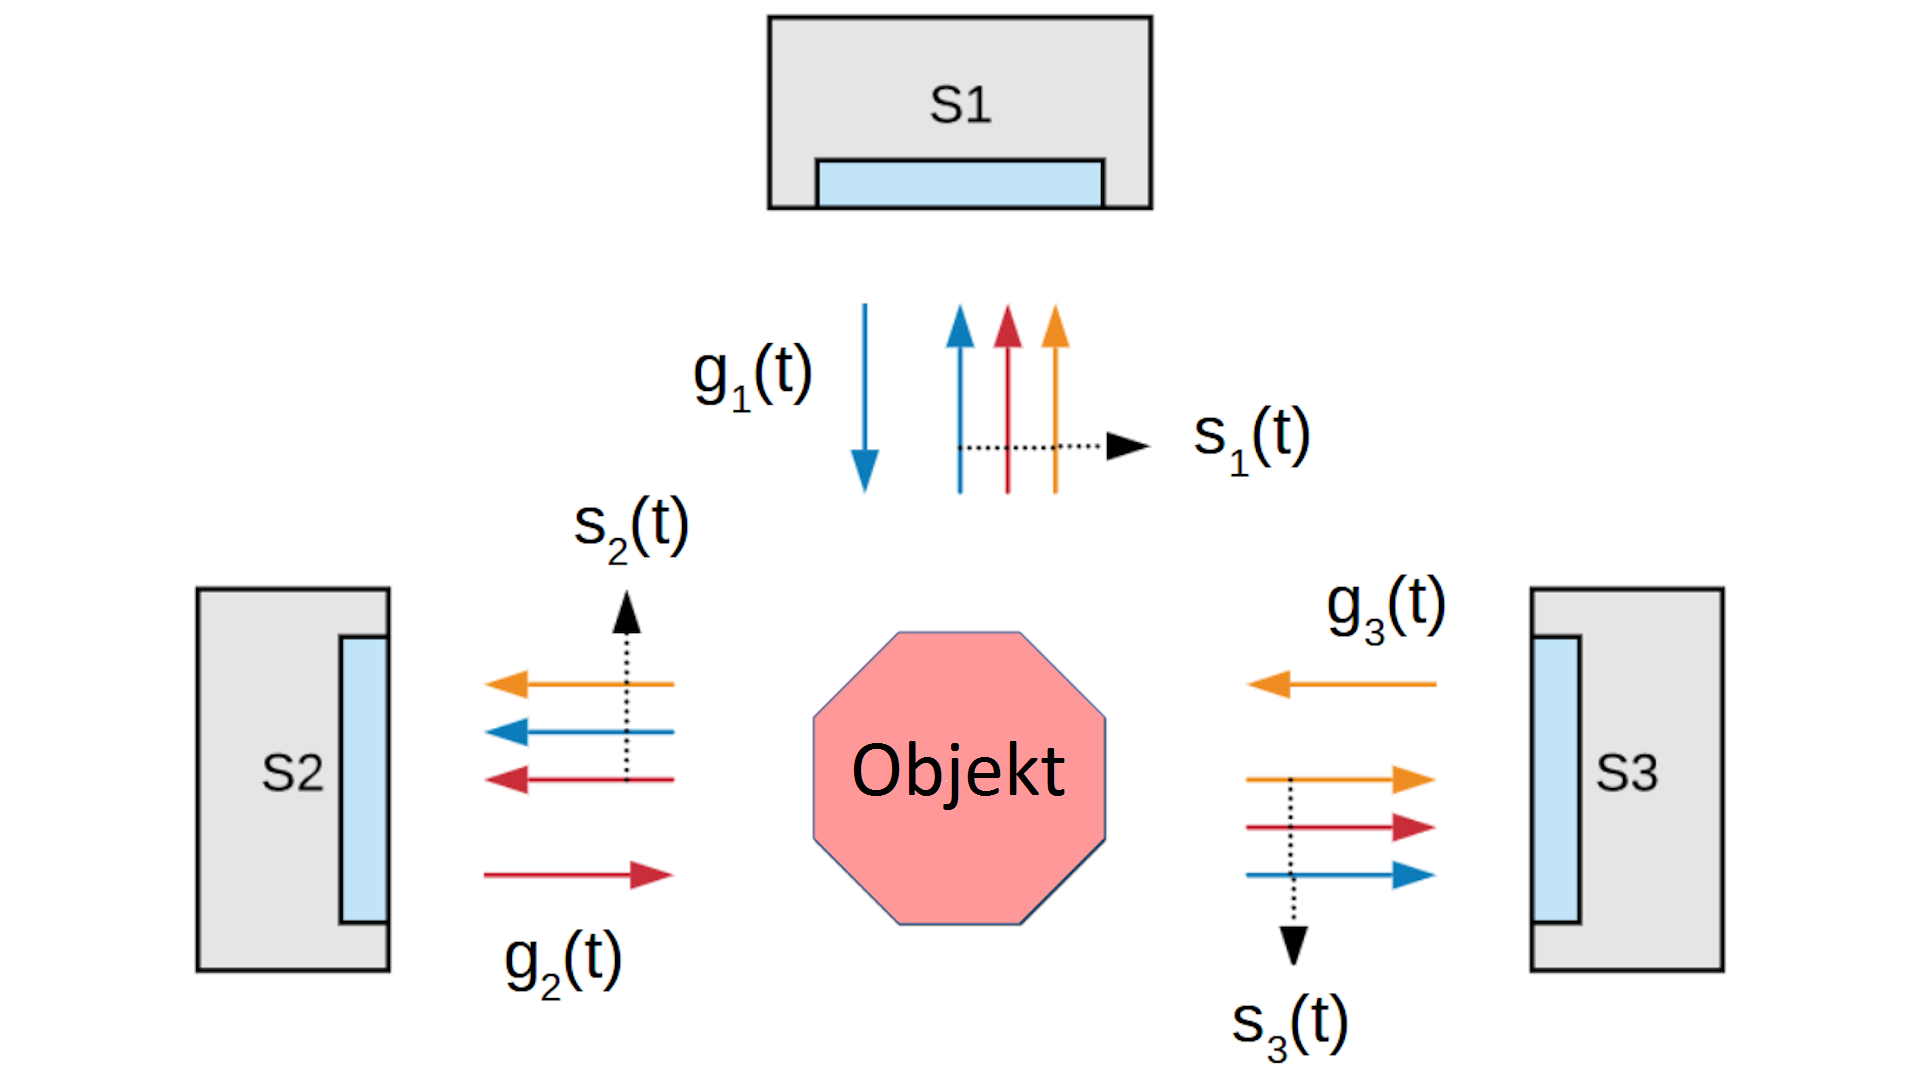
\includegraphics[width=0.74\textwidth]{figures/interference_model.png}
	\caption{Model multi-kamerového systému s interferenciou IR signálu.}
	\label{fig:imodel}
\end{figure}  

Každá kamera generuje signál $g(t)$ a prijíma odrazený signál $s(t)$, ktorý predstavuje spojenie generovaných čiastkových signálov zo všetkých kamier $S$. Tieto signály možno opísať takto:

\begin{equation}
\label{eq::tof::10}
\begin{aligned}
s_1 (t) }= {s_{11}(t)+s_{12}(t)+s_{13}(t) \\
s_2 (t) }= {s_{21}(t)+s_{22}(t)+s_{23}(t) \\
s_3 (t) }= {s_{31}(t)+s_{32}(t)+s_{33}(t) 
\end{aligned}
\end{equation}

\noindent  Každý čiastkový signál možno zapísať ako:

\begin{equation}
\label{eq::tof::11}
\begin{aligned}
s_{xy}(t) = b_{xy}+a_{xy} \cdot cos(\omega t - \varphi _{xy})
\end{aligned}
\end{equation}

Index $x$ predstavuje cieľovú kameru a index $y$ kameru pôvodného signálu. Nasledujúce rovnice slúžia ako príklad výpočtu modelu pre jeden signál $s_1$. Pre ostatné kamery sa matematický model odvodzuje rovnakým spôsobom:

\begin{equation}
\label{eq::tof::12}
\begin{aligned}
&{s_{1}(t) }= {b_{11}+a_{11} \cdot cos(\omega t - \varphi _{11}) + {b_{12} +a_{12} \cdot cos(\omega t - \varphi _{12})}} \\ 
&+ {{b_{13}+a_{13} \cdot cos(\omega t - \varphi _{13})} = \Tilde{b}_1 + \Tilde{a}_1 \cdot cos(\omega t - \Tilde{\varphi_1})}  
\end{aligned}
\end{equation}

\noindent  Po 4-fázovej korelácii rušivých signálov sa rovnice \ref{eq::tof::07} a \ref{eq::tof::08} transformujú do nasledujúcej podoby:

\begin{equation}
\label{eq::tof::13}
\begin{aligned}
&{ \Tilde{\varphi}_1}= atan \Bigg[ {\frac{a_{11}  sin( \tau _{11}) + a_{12}  sin( \tau _{12}) + a_{13}  sin( \tau _{13})}{a_{11}  cos( \tau _{11}) + a_{12}  cos( \tau _{12}) + a_{13}  sin( \tau _{13}) }} \Bigg]
\end{aligned}
\end{equation}

\begin{equation}
\label{eq::tof::14}
\begin{aligned}
&\Tilde{ a_1 }= {\sqrt{\frac{a_{11}^2+a_{12}^2+a_{13}^2 + 2\bar{a}}{2} }}
\end{aligned}
\end{equation}

\noindent kde

\begin{equation}
\label{eq::tof::15}
\begin{aligned}
&{\bar{a}} = {a_{11}a_{12}[sin({\varphi_{11}+\varphi_{12}}) + cos({\varphi_{11}+\varphi_{12}})]} + \\  
&{a_{11}a_{13}[sin({\varphi_{11}+\varphi_{13}}) + cos ({\varphi_{11}+\varphi_{13}})]} + \\
&{a_{12}a_{13}[sin({\varphi_{12}+\varphi_{13}}) + cos ({\varphi_{12}+\varphi_{13}})]}
\end{aligned}
\end{equation}

Toto zmiešanie signálov z rôznych kamier spôsobuje značné chyby merania a preto mapa výstupnej hĺbky obsahuje artefakty \cite{Lianhua}.

\section{Analýza multi-kamerovej interferencie}

Rovnice \ref{eq::tof::13} a \ref{eq::tof::14} sú platné, ak každý prijatý signál $s_{x}(t)$ je kombináciou čiastkových signálov všetkých kamier S1\, - \,S3, kde $x$ sa pohybuje od 1 do 3.
Interakcia signálov úzko súvisí aj so snímanou scénou. Ak si predstavíme priestorové rozloženie kamier, ktoré je znázornené na obr. \ref{fig:imodel}, môžeme popísať určité situácie nastávajúce pri skenovaní. Ak sa v scéne nenachádza objekt, je veľmi veľká pravdepodobnosť že k interferencii dôjde medzi kamerami S2 a S3. Taktiež ak je veľkosť objektu malá a vyžarovanému IR svetlu nebude v ceste stáť žiadna prekážka. Naopak veľký objekt môže zabrániť interferencii medzi kamerami S2 a S3. Veľmi rizikové su aj predmety a povrchy, ktoré reflektujú IR svetlo. Pri skenovaní dynamických objektov sa môže vplyv rušenia meniť, takže filtračný algoritmus musí reagovať na zmeny v čo najkratšom čase.

Ako už bolo spomenuté, výstupom ToF kamier je IR a hĺbkový obraz.  Hĺbkový obraz obsahuje 3D informácie v 2D rovine obrazu. Hodnota jednotlivých pixelov (32-bit float) predstavuje absolútnu vzdialenosť. Na základe týchto informácií je možné znovu premietať naskenovanú scénu, kde musia byť známe interné a externé parametre IR kamery (pozri kapitolu \ref{kap:kalibracia}).

\begin{figure}[h]
	\centering
	\begin{subfigure}[b]{0.2\textwidth}
		\centering
		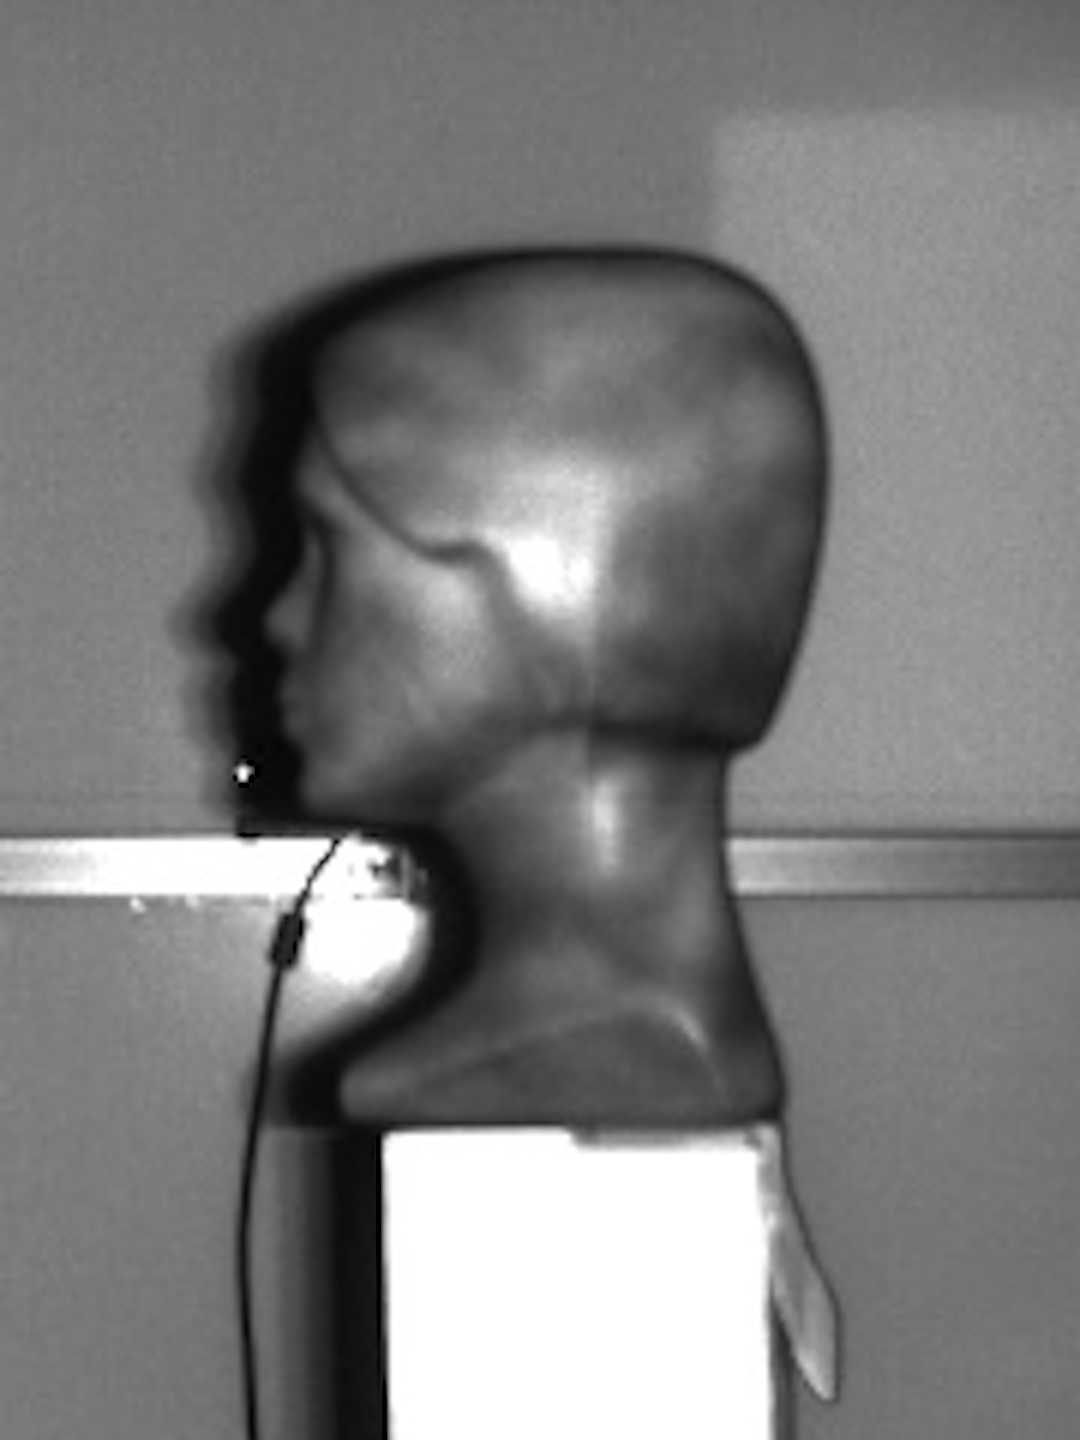
\includegraphics[width=\textwidth]{figures/depth_ir-a.png}
		\caption{}
		\label{fig:depthir:a}
	\end{subfigure}
	\hfill
	\begin{subfigure}[b]{0.2\textwidth}
		\centering
		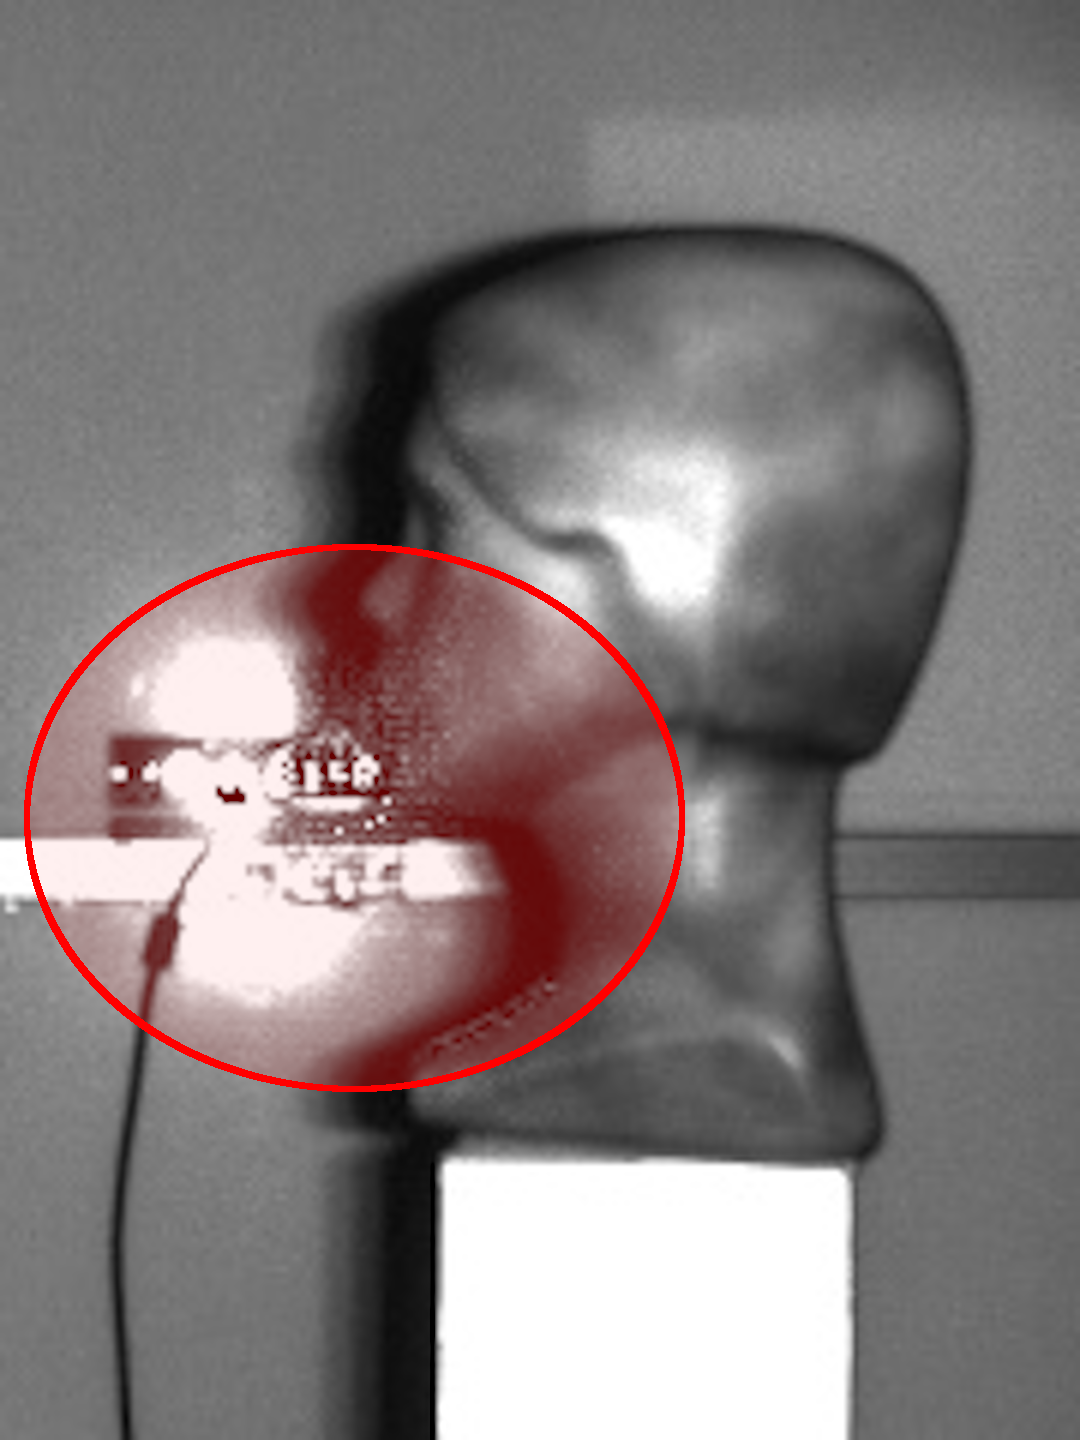
\includegraphics[width=\textwidth]{figures/depth_ir-b.png}
		\caption{}
		\label{fig:depthir:b}
	\end{subfigure}
	\hfill
	\begin{subfigure}[b]{0.2\textwidth}
		\centering
		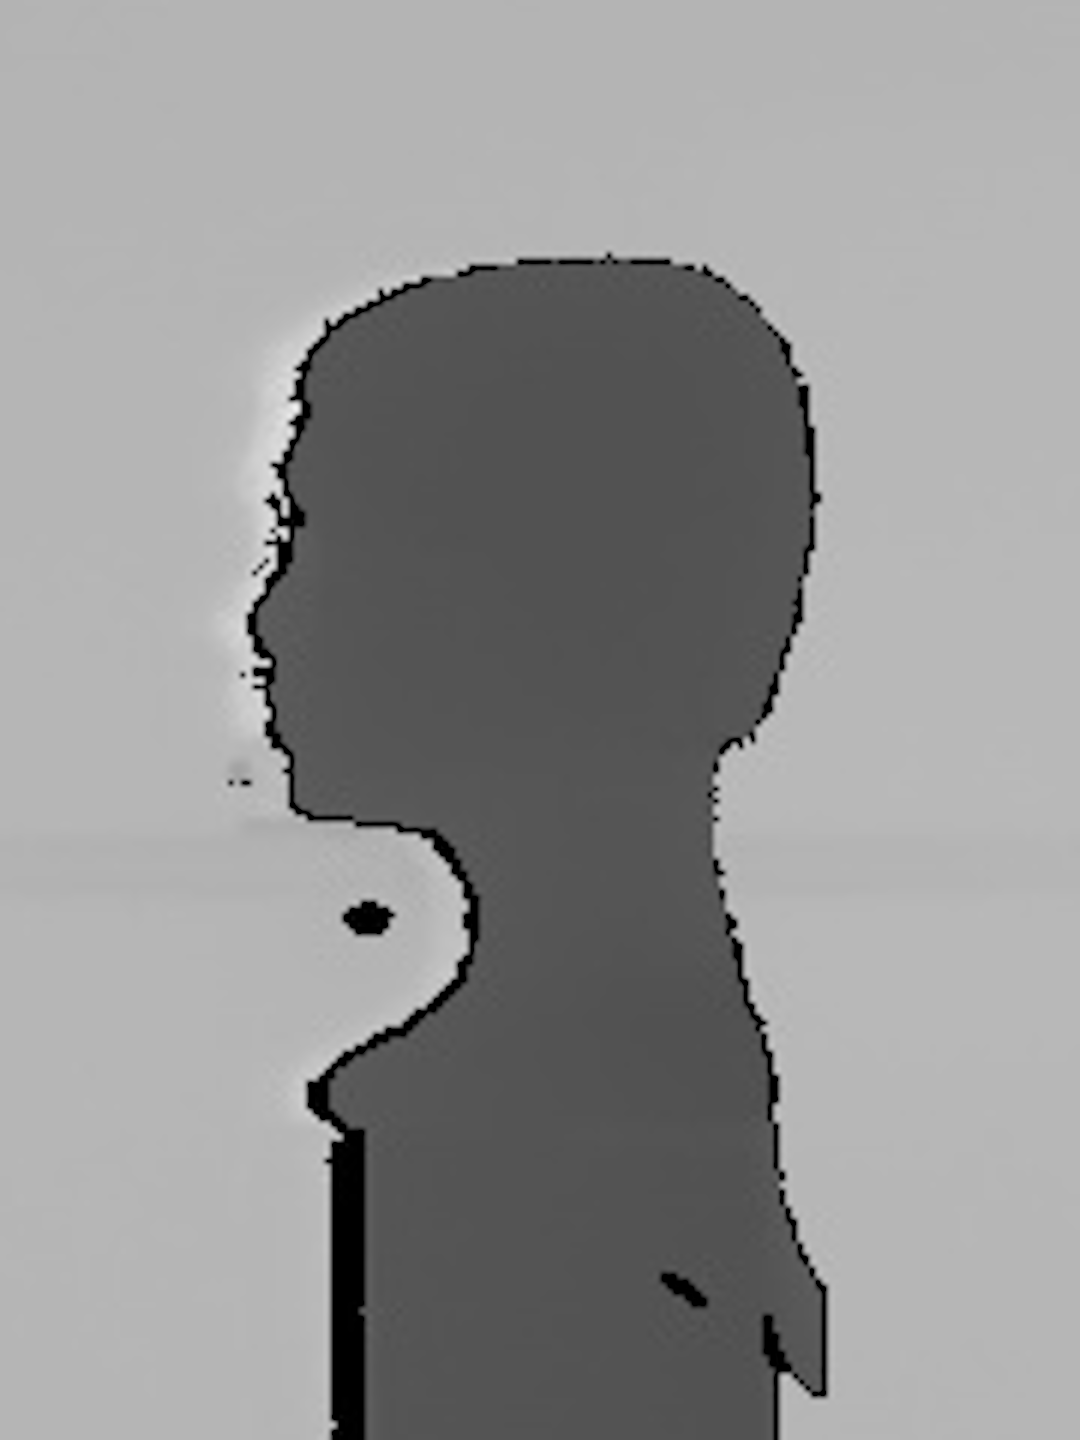
\includegraphics[width=\textwidth]{figures/depth_ir-c.png}
		\caption{}
		\label{fig:depthir:c}
	\end{subfigure}
	\hfill
	\begin{subfigure}[b]{0.2\textwidth}
		\centering
		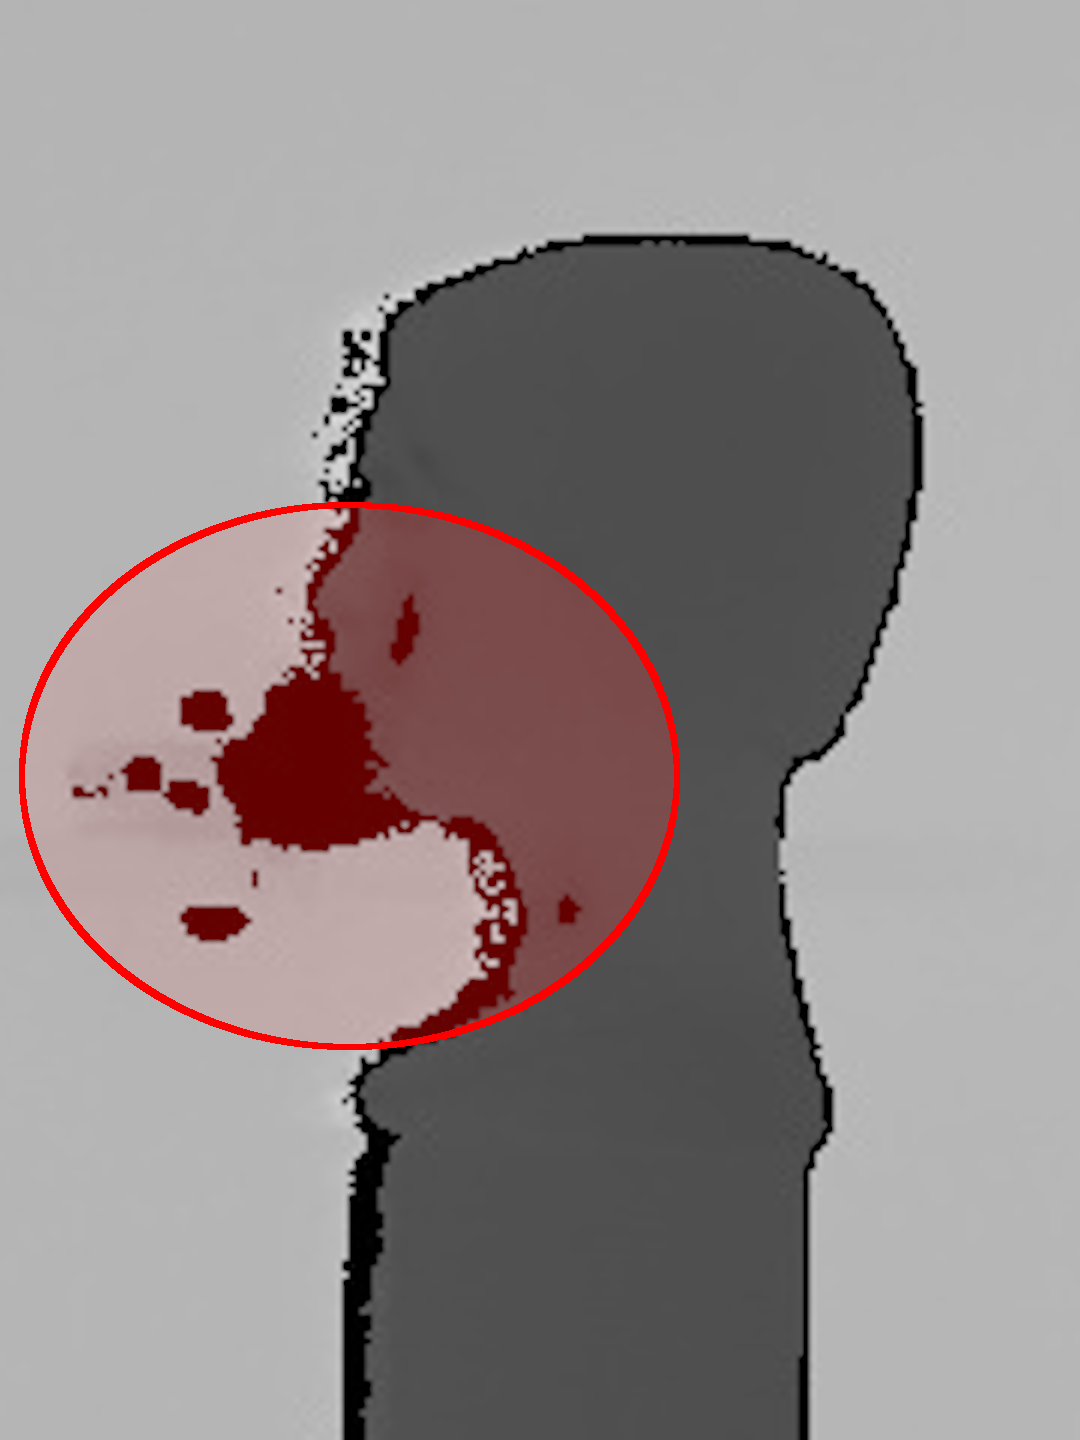
\includegraphics[width=\textwidth]{figures/depth_ir-d.png}
		\caption{}
		\label{fig:depthir:d}
	\end{subfigure}
	\caption{Obrazy zo senzora Microsoft Kinect v2: (\textbf{a}) IR obraz bez interferencie. (\textbf{b}) IR obraz s interferenciou. (\textbf{c}) Hĺbková mapa IR obrazu (a). (\textbf{d}) Hĺbková mapa IR obrazu (b). Miesto interferencie je zvýraznené červenou farbou.}
	\label{fig:depthir}
\end{figure}

Interferencia sa prejavuje na IR obraze, čo ma priamy dopad na výsledný hĺbkový obraz (pozri obr. \ref{fig:depthir}). V hĺbkovom obraze sa v poškodenom mieste objavia pixely, ktoré naberajú extrémne odlišné hodnoty od tých skutočných. Tie sú buď negatívne alebo pozitívne, pričom sa zvyknú pulzovaním striedať. 

\begin{figure}[h]
	\centering
	\begin{subfigure}[b]{0.24\textwidth}
		\centering
		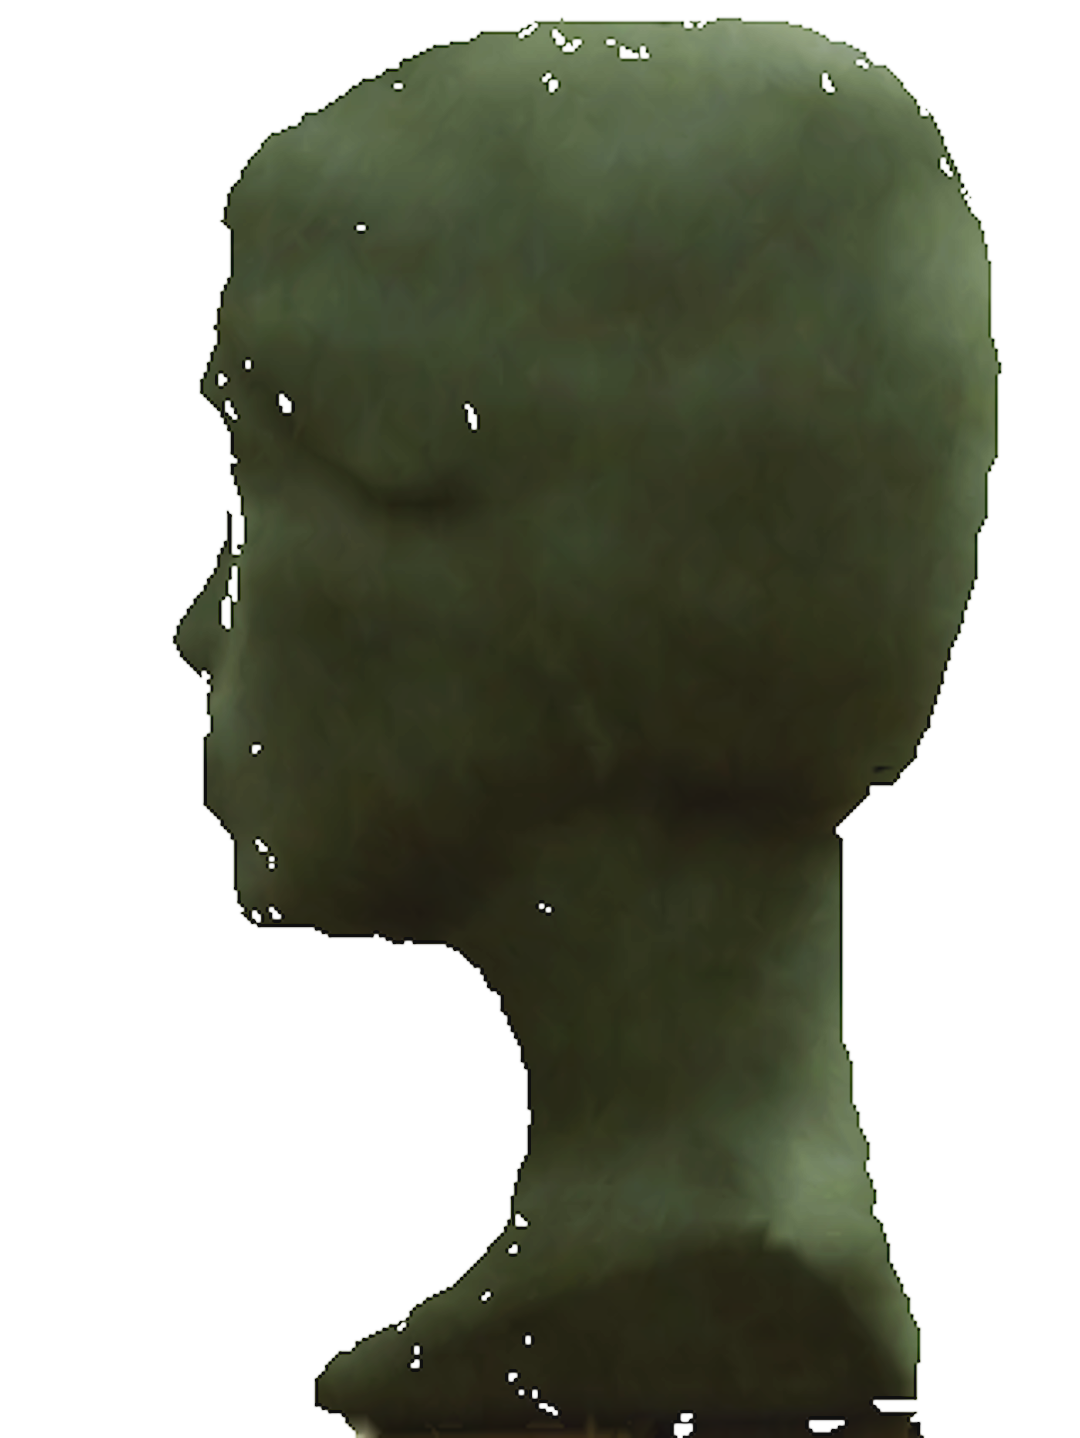
\includegraphics[width=0.7\textwidth]{figures/3dmodels-c.png}
		\caption{}
		\label{fig:3dm:b}
	\end{subfigure}
	\hfill
	\begin{subfigure}[b]{0.24\textwidth}
		\centering
		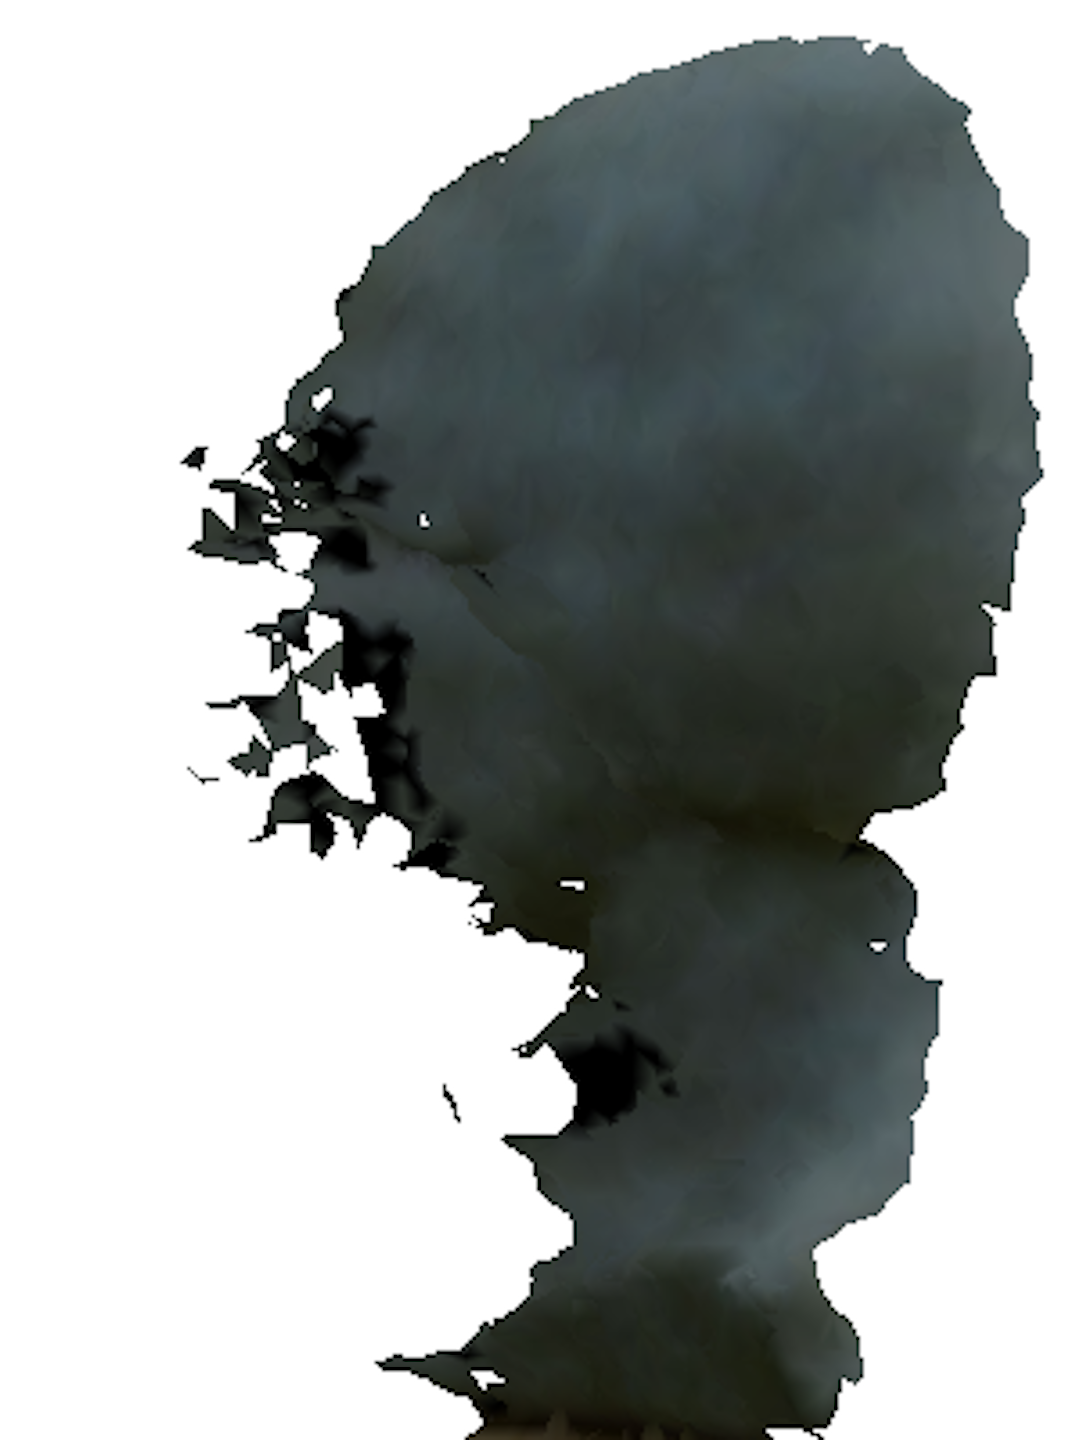
\includegraphics[width=0.7\textwidth]{figures/3dmodels-a.png}
		\caption{}
		\label{fig:3dm:a}
	\end{subfigure}
	\hfill
	\begin{subfigure}[b]{0.24\textwidth}
		\centering
		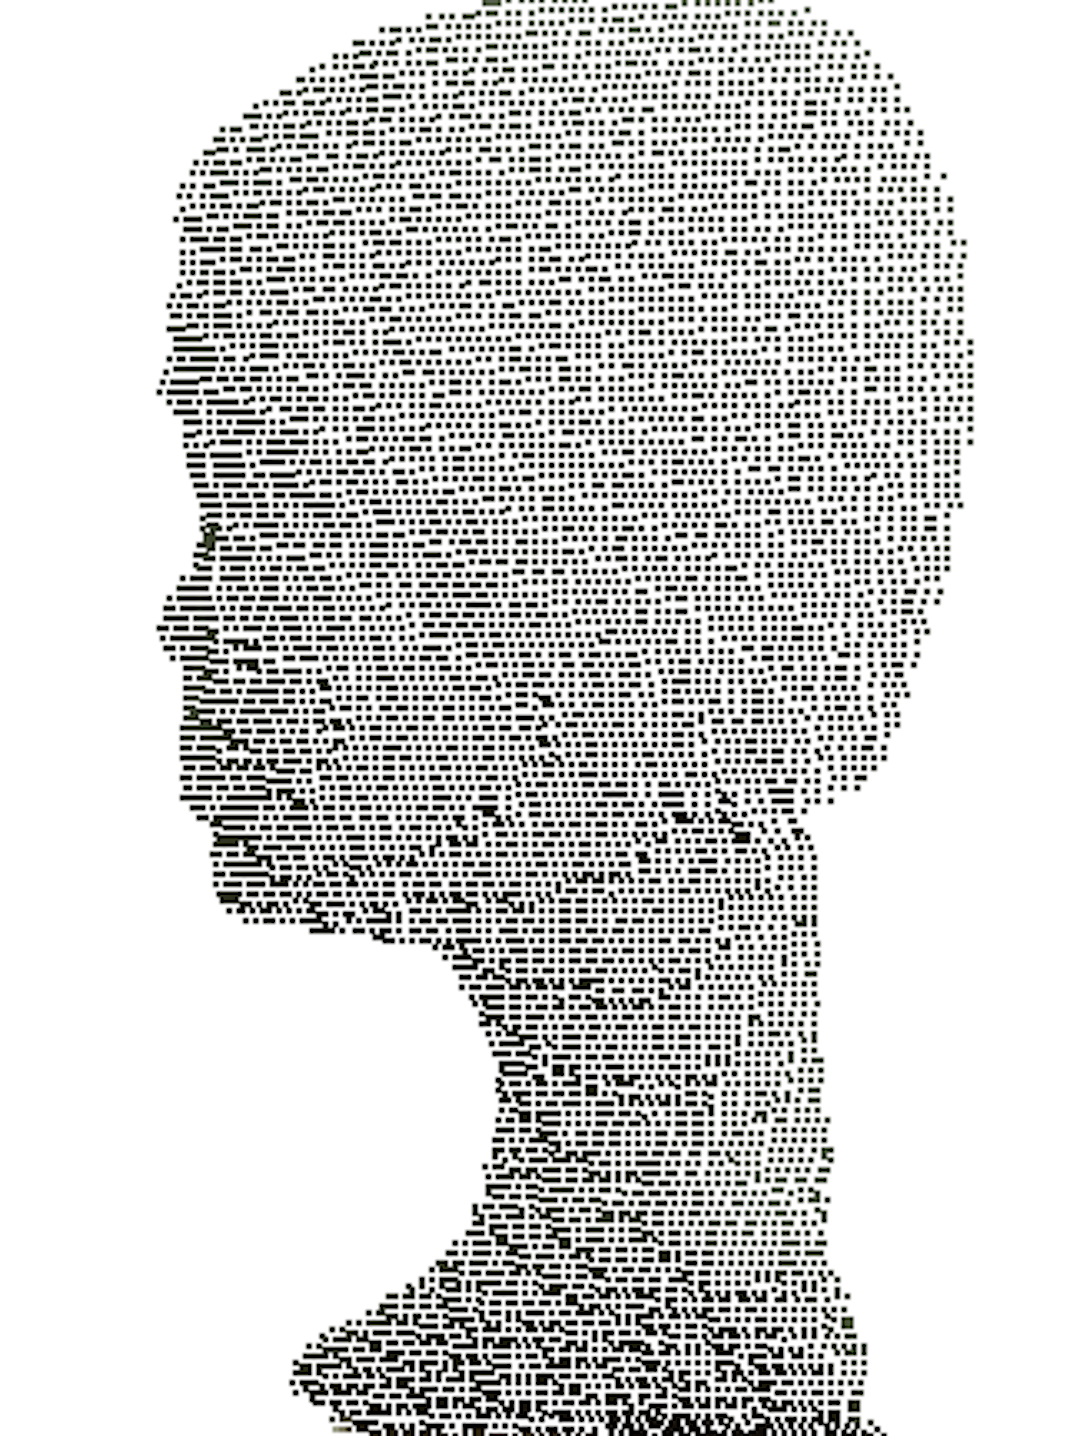
\includegraphics[width=0.7\textwidth]{figures/3dmodels-d.png}
		\caption{}
		\label{fig:3dm:d}
	\end{subfigure}
	\hfill
	\begin{subfigure}[b]{0.24\textwidth}
		\centering
		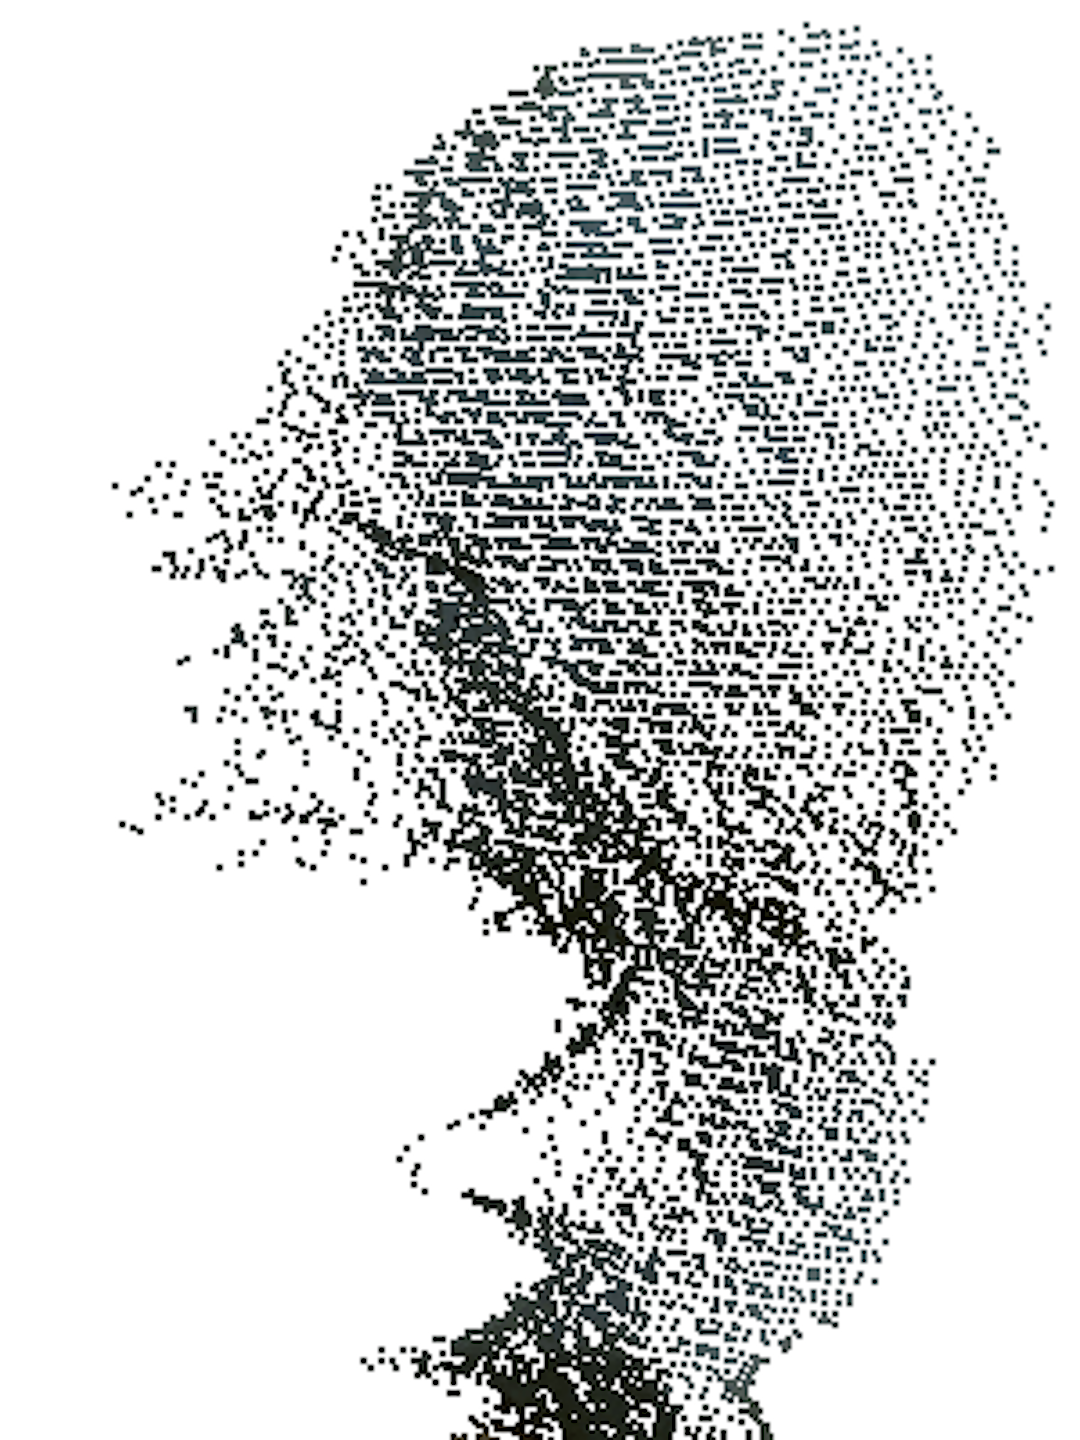
\includegraphics[width=0.7\textwidth]{figures/3dmodels-b.png}
		\caption{}
		\label{fig:3dm:c}
	\end{subfigure}
	\caption{Rekonštruovaný 3D model statického objektu: (\textbf{a}) 3D trojuholníková sieť objektu bez interferencie. (\textbf{b}) 3D trojuholníková sieť objektu s interferenciou. (\textbf{c}) Mračno bodov objektu bez interferencie. (\textbf{d}) Mračno bodov objektu s interferenciou.}
	\label{fig:3dmodel}
\end{figure}

Pri pozitívnej interferencii môže ísť hĺbka do maximálnych možných hodnôt (32-bit float), pri negatívnej môže ísť do 0. Tieto miesta sú zároveň obkolesené deformovanými pixelmi, ktoré nenaberajú extrémne hodnoty, ale stále výrazne zhoršujú kvalitu výstupného modelu. Grafické znázornenie v 3D priestore je možné vidieť na obrázkoch \ref{fig:3dm:b} a \ref{fig:3dm:d}. Práve tieto miesta sú veľmi kritické, pretože ich identifikácia je problematická. 

\section{Filtračné metódy}
\label{sec:filtmethods}

Existuje niekoľko prehľadových článkov, ktoré sa zaoberajú technikami filtrácie a obnovy používanými pri 3D zobrazovaní a skenovaní. Zo všetkých z nich sa práca \cite{Han} javí ako veľmi užitočná, pretože obsahuje prehľad približne 40 metód a rozdeľuje ich do niekoľkých tried. Mnohé z týchto metód sú použiteľné na 3D mračná bodov, avšak žiadny známy nie je priamo určený pre potláčanie interferencie. Na tento účel bol navrhnutý IMBM filter, ktorý sa môže zaradiť medzi štatistické filtre. Pre porovnanie sú v tejto práci opísané ďalšie filtračné metódy založené na štatistike (SOR, ROR) alebo na princípoch umelej inteligencie (PointCleanNet).   

\subsection{SOR filter}

Filtračná metóda SOR (Statistical Outlier Removal) je založená na štatistickej analýze okolia každého bodu. Odľahlá hodnota sa dá klasifikovať ako stratený alebo izolovaný bod, poprípade ako súbor bodov v mračne. V SOR metóde sa určuje počet bodov, ktoré sa budú považovať za susedov (definovaný počet $k$ najbližších susedov \cite{Pirotti}) a potom sa vypočíta priemerná vzdialenosť každého bodu od jeho susedov. Body, ktorých stredné vzdialenosti nespĺňajú kritériá a sú mimo intervalu sa považujú za odľahlé. Interval je definovaný strednou hodnotou stredných vzdialeností a štandardnou odchýlkou \cite{Corso}. SOR je široko používaná a efektívna metóda, aj keď vo veľkých množinách 3D dát je časovo neefektívna  \cite{Balta}.

\subsection{ROR filter}
Metóda ROR (Radius Outlier Removal) predstavuje pomerne jednoduchý štatistický filter. Do filtra sa zadávajú parametre sférického polomeru $rad$ a minimálneho počtu susedov $pts$. Filter odstráni body, ktoré majú v oblasti polomeru $rad$ menej susedných bodov ako bolo nastavené parametrom $pts$.


\subsection{PointCleanNet}
PointCleanNet je dvojfázový algoritmus hĺbkového učenia, ktorý odstraňuje odľahlé hodnoty a znižuje šum v neusporiadaných mračnách bodov. Architektúra je založená na PCPNet (prístup založený na hlbokom učení na odhad lokálnych 3D vlastností v mračnách bodov \cite{Guerrero}) s niekoľkými úpravami. V prvom kroku sa odstraňujú odľahlé body, v druhom sa odhadujú korekčné vektory pre zostávajúce body. Trénovanie tejto siete je časovo náročné, taktiež je vyžadované použitie CUDA.

\subsection{Importance Map Based Median filter}

Nami navrhnutý filtračný algoritmus je založený na identifikácií, extrakcii a interpolácií interferenčnej oblasti zo sekvencie hĺbkových máp získaných z ToF senzorov. Cieľom nie je poškodené miesta úplne odstrániť, ale čo najviac minimalizovať vplyv interferencie bez veľkej straty užitočných dát. Primárne využitie filtra je pre aplikáciu skenovania ľudských hláv, ale nie je obmedzené iba na túto činnosť. Základnou požiadavkou je získať dostatočný počet hĺbkových máp do obrazového zásobníka, pričom snímaná scéna nebola výrazne zmenená. Táto podmienka je splnená, ak je snímaný objekt statický alebo v pokoji (pacient nie je v strese). V prípade dynamickej scény je žiadúca minimalizácia veľkosti zásobníka, inač by mohlo dôjsť k vytvoreniu pohybových artefaktov v hĺbkovej mape.

\begin{figure}[h]
	\centering
	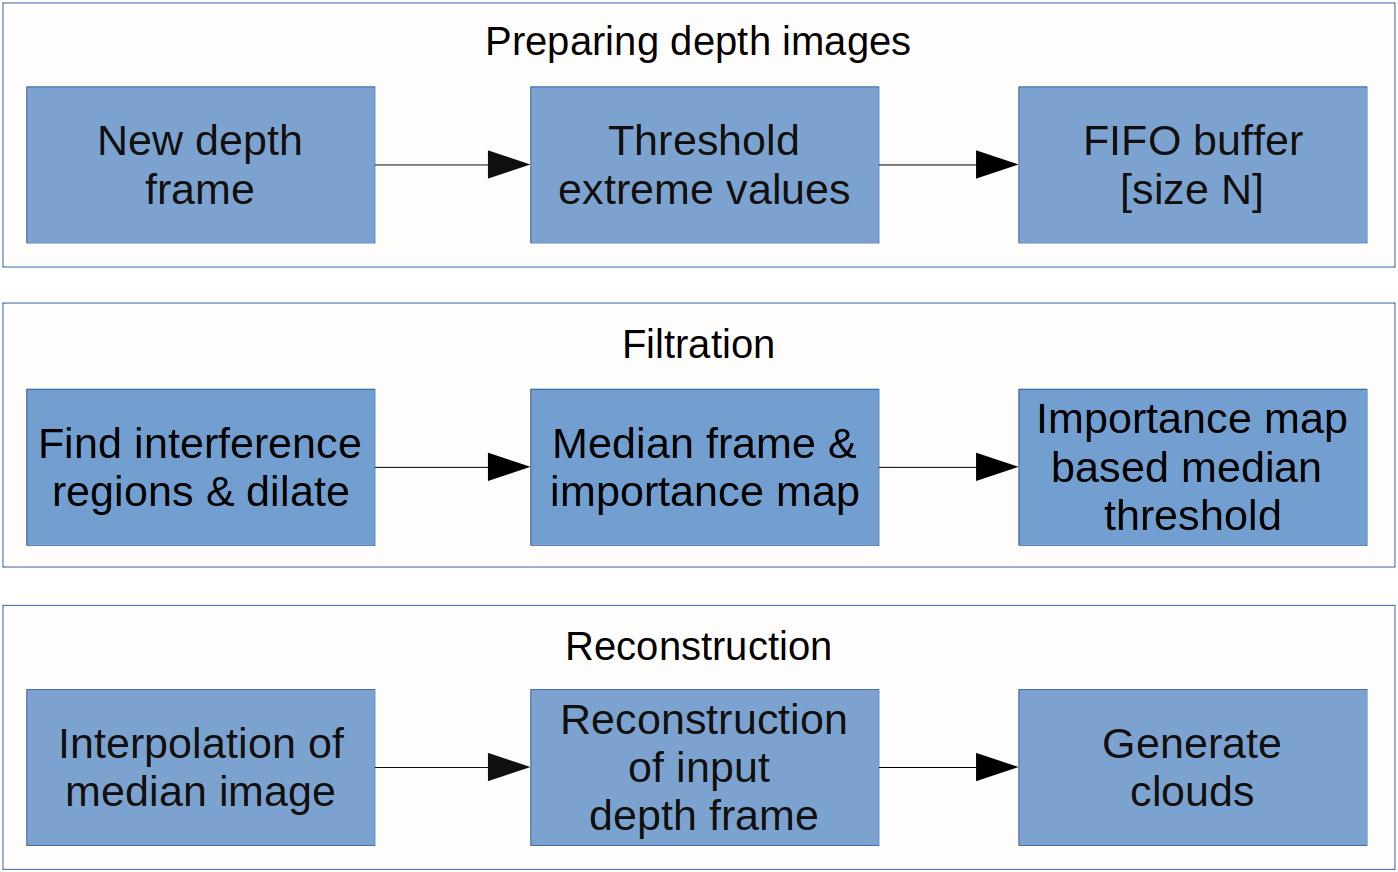
\includegraphics[width=0.75\textwidth]{figures/algorithm.png}
	\caption{Blokový diagram navrhnutého IMBM filtra.}
	\label{fig:algorithm}
\end{figure}

V prvom kroku je potrebné naplniť obrazový zásobník, ktorého veľkosť je špecifikovaná podľa danej snímanej scény a intenzity interferencie. Plnenie funguje na princípe FIFO. Najprv sa zásobník naplní hĺbkovými mapami a po naplnení zásobníka každý nový snímok vylúči ten najstarší, čím je zabezpečená stála veľkosť zásobníka. 
Všetky vstupujúce hĺbkové mapy sú prahované podľa prahových hodnôt určených topológiou a vlastnosťami systému.  

Ak \textit{d(x;y)} predstavuje jednotlivý pixel hĺbkovej mapy, tak je prahovanie vykonávané pomocou rovnice \ref{eq::imbm::threshold}.

\begin{equation}
\label{eq::imbm::threshold}
\begin{aligned}
d'(x;y)=
\begin{cases}
d(x;y), & \text{if}\ d(x;y) \in < T_{LOW}; T_{HIGH}> \\
0, & \text{v inom prípade}
\end{cases}
\end{aligned}
\end{equation}

kde \textit{d(x; y)} je 32-bitové float číslo a $T_{LOW}$, $T_ {HIGH}$ sú dolné a horné prahové hodnoty. V našom prípade sú nastavené na 80 a 1300 (tieto čísla predstavujú skutočnú vzdialenosť v mm). Skenovacia kabína je znázornená na obrázku \ref {fig:cabin} a rozmer spodnej časti je $ 1520 \times 1520$ \, mm.

\begin{figure}[h]
	\centering
	\begin{subfigure}[b]{0.49\textwidth}
		\centering
		\includegraphics[height=5.5cm]{figures/threshold_a.png}
		\caption{}
		\label{fig:threshold:a}
	\end{subfigure}
	\hskip 0pt
	\begin{subfigure}[b]{0.49\textwidth}
		\centering
		\includegraphics[height=5.5cm]{figures/threshold_b.png}
		\caption{}
		\label{fig:threshold:b}
	\end{subfigure}
	\caption{Vplyv prahovania na interferovanú hĺbkovú mapu(\textbf{a}) Hĺbková mapa s interferovanými regiónmi. Pixely nadobúdajú extrémne hodnoty. (\textbf{b}) Hĺbková mapa bez extrémnej interferencie.}
	\label{fig:threshold}
\end{figure}

Po prahovaní hĺbky sa pozadie odstráni a obrázky obsahujú iba predmet záujmu (Obr. \, \ref{fig:threshold}). Tento jednoduchý krok je dôležitý a účinný, pretože odstraňuje oblasti so spomínanou extrémnou interferenciou a pozadia.

V ďalšom kroku sa z obrazového zásobníka vyberie ako referenčný obraz filtrovaná hĺbková mapa s minimálnym počtom nenulových hodnôt. Je to preto, že tento obrázok s najväčšou pravdepodobnosťou obsahuje minimálny počet rušivých pixelov. Z tejto referencie je vytvorená binárna mapa a každá hĺbková mapa je s ňou maskovaná. V tomto kroku sú pixely vstupných máp rozdelené do troch oblastí: pozadie (vrátane extrémnych interferenčných oblastí), pixely interferenčnej oblasti (tiež vrátane niektorých pixelov objektu) a oblasť objektov (vrátane interferenčných pixelov).


\begin{figure}[h]
	\centering
	\begin{subfigure}[b]{0.32\textwidth}
		\centering
		\includegraphics[height=5.2cm]{figures/interf_roi_a.png}
		\caption{}
		\label{fig:interf:a}
	\end{subfigure}
	\hskip 0pt
	\begin{subfigure}[b]{0.32\textwidth}
		\centering
		\includegraphics[height=5.2cm]{figures/interf_roi_b.png}
		\caption{}
		\label{fig:interf:b}
	\end{subfigure}
	\hskip 0pt
	\begin{subfigure}[b]{0.32\textwidth}
		\centering
		\includegraphics[height=5.2cm]{figures/interf_roi_c.png}
		\caption{}
		\label{fig:interf:c}
	\end{subfigure}
	\caption{Identifikácia interferovaných regiónov v hĺbkových mapách. (\textbf{a}) Referenčná mapa s maximálnym počtom 0 pixelov.(\textbf{b}) Vstupná mapa s interferenciou. (\textbf{c}) Mapa zobrazujúca možné interfereované regióny obrazu \textbf{b}.}
	\label{fig:interf}
\end{figure}


Výsledná rozdielová maska je ešte dilatovaná prvkom o štvorcovej štruktúre $ 1 \times1 $, čím sú odstraňované oblasti s nízkou intenzitou interferencie. Týmto spôsobom sa zníži celkový súčet interferenčných pixelov, ale zároveň znižujeme aj súčet správnych obrazových pixelov skenovaného objektu. 

Tieto morfologicky spracované snímky sa používajú na výpočet mediánu hĺbkovej mapy a na vytvorenie mapy dôležitosti pixelov.\newline


\textbf{Pixel mediánu hĺbkovej mapy} je vypočítavaný ako medián všetkých konkrétnych nenulových pixelov (rovnaká pozícia riadku a stĺpca v obraze) hĺbkových máp v zásobníku. \newline

\textbf{Mapa dôležitosti pixelov} nám hovorí, z koľkých hodnôt boli vypočítané konkrétne pixely v mediáne hĺbkovej mapy.  Malá hodnota dôležitosti daného pixelu znamená vysokú pravdepodobnosť interferencie vyskytujúcej sa v určitom bode. Z tohto dôvodu sa zdá byť užitočné odstrániť také oblasti nastavením prahu dôležitosti.


\begin{figure}[h]
	\centering
	\begin{subfigure}[b]{0.32\textwidth}
		\centering
		\includegraphics[height=5.2cm]{figures/importance_map-a.png}
		\caption{}
		\label{fig:imap:a}
	\end{subfigure}
	\hfill
	\begin{subfigure}[b]{0.32\textwidth}
		\centering
		\includegraphics[height=5.2cm]{figures/importance_map-b.png}
		\caption{}
		\label{fig:imap:b}
	\end{subfigure}
	\hfill
	\begin{subfigure}[b]{0.32\textwidth}
		\centering
		\includegraphics[height=5.2cm]{figures/importance_map-c.png}
		\caption{}
		\label{fig:imap:c}
	\end{subfigure}
	\caption{Filtrácia a interpolácia hĺbkových máp. (\textbf{a}) Mapa dôležitosti. (\textbf{b}) Medián. (\textbf{c}) Interpolovaná mediánová hĺbková mapa.}
	\label{fig:imap}
\end{figure}

Pixely v mediáne (Obr. \, \ref{fig:imap:b}) s vybranou dôležitosťou vyššou ako $ k \cdot \, N $ sú zachované, ostatné pixely sú nastavené na nulu. $K$ predstavuje prahovú hodnotu dôležitosti mapy a $N$ je veľkosť obrazového zásobníka. Koeficient $k$ môže mať rozsah hodnôt od 0 do 1. Tento krok je posledný, znižuje vplyv interferencie na hĺbkové mapy. Ostatné časti filtračného algoritmu zabezpečujú rekonštrukciu filtrovaných dát, ale nie sú nevyhnutné. 

Interpolácia filtrovaných miest je nasledujúcim krokom IMBM. Rekonštrukcia dát využíva bilineárnu interpoláciu \cite{Volak2019}, pričom tá je vykonávaná iba na špecifických filtrovaných miestach spĺňajúcich definované podmienky. K obmedzeniu interpolácie dochádza na neuzavretých dierach, pri veľkých dierach a pri vysokých rozdieloch medzi interpolačnými pixelmi. Bilineárna interpolácia môže byť nahradená inou metódou interpolácie (napr. Bikubická, biquadratická ...). Z hľadiska výpočtu je bilineárna transformácia dobrým kompromisom medzi metódou najbližšieho suseda a inými zložitejšími metódami interpolácie.

Mediánom môžeme opraviť vstupné hĺbkové mapy. Tým opravíme nie len interferované miesta ale aj znížime vplyv šumu kamier. V procese opravy sa pixely hĺbkových máp porovnávajú s pixelmi mediánu. Ak je absolútna hodnota rozdielu väčšia ako zvolená šumová prahová hodnota (táto premenná je diskutovaná v experimentálnej časti \ref{sec:imbm:filtration}), pixel v pôvodnej hĺbkovej mape sa nahradí mediánovou hodnotou (alebo nulovou hodnotou, v závislosti od režimu metódy IMBM).

Hodnota šumového prahu závisí od intenzity šumu kamery pre definovanú vzdialenosť. Ak je táto hodnota príliš nízka, veľký počet neinterferujúcich pixelov bude nahradený strednou hodnotou. Na druhej strane by filter mohol zachovať veľké množstvo rušenia v pôvodnom obraze.

Všeobecne možno povedať, že použitie navrhovaného algoritmu zlepšuje hĺbkový obraz (Obr. \, \ref{fig:imap:c}) znížením lietajúcich pixelov, šumových procesov a vyplnením dier vo výslednom 3D modeli.


\section{Nastavenie experimentu}

Na overenie funkčnosti vybraných metód filtrácie sme vykonali experiment v reálnych podmienkach na statickom objekte. V experimente boli použité tri ToF kamery typu Microsoft Kinect v2. Tie boli umiestnené do skenovacej kabíny, ktorej návrh je zobrazený na obrázku \ref{fig:cabin}. V strede kabíny je modelový objekt umiestnený v rozsahu od 60 \ cm do 80 \ cm od senzorov. Predmetom bola plastová hlava s pomerne komplexným tvarom. Veľkosť objektu zodpovedá normálnym rozmerom dieťaťa vo veku 5-10 rokov.

\begin{figure}[H]
	\centering
	\tabskip=0pt
	\valign{#\cr
		\hbox{%
			\begin{subfigure}[b]{0.28\textwidth}
				\centering
				\includegraphics[height=8cm]{figures/ground_truth-a.png}
				\caption{}
				\label{fig:gt:a}
			\end{subfigure}
		}\cr
		\hbox{%
			\begin{subfigure}[b]{0.28\textwidth}
				\centering
				\includegraphics[height=8cm]{figures/ground_truth-b.png}
				\caption{}
				\label{fig:gt:b}
			\end{subfigure}
		}\cr
		\hbox{%
			\begin{subfigure}{.4\textwidth}
				\centering
				\includegraphics[height=3.5cm]{figures/reference.png}
				\caption{}
				\label{fig:reference}
			\end{subfigure}%
		}\vfill
		\hbox{%
			\begin{subfigure}{.4\textwidth}
				\centering
				\includegraphics[height=3.5cm]{figures/kinect_cabin.png}
				\caption{}
				\label{fig:cabin}
			\end{subfigure}%
		}\cr
	}
	
	\caption{Referenčné obrazy multi-kamerovej sústavy: (\textbf{a}) RGB snímky. (\textbf{b}) Hĺbkové mapy. (\textbf{c}) 3D model vytvorený z hĺbkových máp. (\textbf{d}) Konštrukcia skenovacej kabíny s ukážkou rozloženia kamier.}
	\label{fig:gt}
\end{figure}

RGB obrázky prijaté z každej kamery sú znázornené na obrázku \ref {fig:gt:a}, hĺbkové snímky snímanej scény bez rušenia (postupne pracujúce kamery) pre jednotlivé kamery sú uvedené na obrázku \ref {fig:gt:b}. Tieto hĺbkové mapy sa použili ako referenčné údaje bez interferenčných artefaktov. Obrázok \ref{fig:reference} je rekonštruovaný 3D model statického objektu.

Aby bolo možné objektívne vyhodnotiť výkon potlačenia rušenia, musí sa identifikovať povaha každého bodu v mračne bodov. Zisťuje či ide alebo nejde o skutočné rušenie. Dáta skreslené interferenciou sa získali v režime paralelného snímania. Pre získanie tejto informácie sme použili priestorové porovnávanie interferovaných dát voči referenčným. Referenčná sieť, znázornená na obrázku \ref {fig:reference}, bola získaná z mračna referenčných bodov. Celkový proces vyhodnotenia metód je uvedený na obrázku \ref{fig:eval}.

\begin{figure}[H]
	\centering
	\includegraphics[width=\textwidth]{figures/eval.png}
	\caption{Blokový diagram vyhodnocovacieho procesu.}
	\label{fig:eval}
\end{figure}

\noindent Kroky v tomto procese sú opísané nasledovne:

\begin{itemize}
	\item \textbf{Zásobník} - zachytenie niekoľkých mračien bodov z konkrétneho pohľadu a zlúčenie do jedného mračna.
	\item \textbf{Filtrovanie} - použitie jednej z metód filtrovania opísaných v podkapitole \ref{sec:filtmethods}.
	\item \textbf{Porovnanie s referenciou} - výpočet Hausdorffových vzdialeností voči referenčnej sieti pre konkrétny pohľad.
	\item \textbf{Priestorové filtrovanie} - štatistické rozhodnutie, či ide o rušenie alebo nie na základe Hausdorffovej vzdialenosti. Za rušenie sa považujú štatistické odľahlé hodnoty.
	\item \textbf{Analýza} - vyhodnotenie výsledkov pomocou známych metrík z ROC analýzy.
\end{itemize}

V experimentálnej časti používame na hodnotenie výkonnosti konkrétnych metód nasledujúce metriky.

\begin{itemize}
	\item \textbf{Accuracy} odráža celkový výkon algoritmu, takže zohľadňuje aj skutočné negatívne predpovede (bod nie je interferovaný). Presnosť je vysoká, keď je počet skutočných pozitívnych a pravdivých negatívnych predpovedí vysoký.
	
	\item \textbf{Recall} predstavuje počet odstránených bodov, ktoré boli interferované. Nezohľadňuje ale počet falošne pozitívnych odstránených bodov. Recall je vysoké, keď je počet skutočných predpovedí (filtrovaných interferenčných bodov) veľký, bez ohľadu na to, koľko užitočných bodov stratíme.
	
	\item \textbf{Precision} odráža počet skutočných predpovedí s ohľadom na počet falošne pozitívnych predpovedí.
	
	\item \textbf{F1 score} je hodnota rovnováhy medzi Recall a Precision. To znamená, že skóre F1 nie je skreslené veľkým počtom skutočne negatívnych predpovedí a môže sa považovať za rozhodujúce.
	
	\item \textbf{Hausdorffova vzdialenosť} meria euklidovskú vzdialenosť dvoch vzájomné porovnávaných bodov. Používa sa stredná hodnota vzdialenosti od bodu v mračne k najbližšiemu povrchu v referenčnej sieti .
\end{itemize}

\section{Výsledky experimentu}

V prvom kroku testovania sa hľadali optimálne nastavenia vstupných parametrov pre jednotlivé filtre. Automatickou rekonfiguráciou sa získali rôzne kombinácie nastavení, z ktorých boli následne vybrané najoptimálnejšie parametre (najlepšie F1 skóre). Vysoká hodnota Accuracy môže byť v tomto prípade zavádzajúci parameter, pretože veľké množstvo TN predikcií skresľuje výsledok. Taktiež nízka Hausdorffová vzdialenosť nemusí automaticky znamenať vysoký výkon filtra. Pri použití Hausforffovej vzdialenosti nevidíme, koľko užitočných bodov bolo zbytočne odstránených. Príklad rozdielu v hodnotení pomocou Hausdorffovej vzdialenosti a F1 skóre je vidieť na obr. \ref{fig:sor_hausdorff}. 


\begin{figure}[h]
	\centering
	\begin{subfigure}[b]{0.32\textwidth}
		\centering
		\includegraphics[height=4cm]{figures/sorinterf.png}
		\caption{}
		\label{fig:sor_hausdorff:a}
	\end{subfigure}
	\hfill
	\begin{subfigure}[b]{0.32\textwidth}
		\centering
		\includegraphics[height=4cm]{figures/soridealfilt.png}
		\caption{}
		\label{fig:sor_hausdorff:b}
	\end{subfigure}
	\hfill
	\begin{subfigure}[b]{0.32\textwidth}
		\centering
		\includegraphics[height=4cm]{figures/soroverfilt.png}
		\caption{}
		\label{fig:sor_hausdorff:c}
	\end{subfigure}
	\caption{Rozdiel v hodnotení výkonnosti filtrácie pomocou Hausdorffovej vzdialenosti a F1 skóre. (\textbf{a}) Mračno bodov s interferenciou. Priemerná Hausdorffova vzdialenosť je veľká. (\textbf{b}) Filtrované mračno bodov. Priemerná Hausdorffova vzdialenosť je nízka a skóre F1 je veľké. (\textbf{c}) Filtrované mračno bodov s veľkou stratou užitočných bodov. Priemerná Hausdorffova vzdialenosť je nízka, skóre F1 je nízke.}
	\label{fig:sor_hausdorff}
\end{figure}

Meranie doby spracovania dát sa uskutočňovalo na operačnom systéme Ubuntu s procesorom Intel® Core ™ i5-6440HQ 2,60 GHz a 16 GB operačnej pamäte. 

\subsection{SOR filtrácia}

Filter SOR nám umožňuje upraviť $sdm$ -parameter (prahová hodnota multiplikátora štandardnej odchýlky) a $k$ -parameter (počet bodov, ktoré sa majú použiť na odhad priemernej vzdialenosti). Nasledujúce farebné mapy (Obr. \ref{fig:sorf1}) ukazujú, ako sa mení výkon filtrácie vyhodnotený ako skóre F1 v závislosti od výberu parametrov a veľkosti vyrovnávacej pamäte.

\begin{figure}[h]
	\centering
	\includegraphics[width=\textwidth]{figures/sor_f1.png}
	\caption{Farebná mapa závislosti F1 skóre od vstupných parametrov SOR filtra pre každú veľkosť obrazového zásobníka.}
	\label{fig:sorf1}
\end{figure}

\begin{table}[h]
	\centering
	\caption{\label{tab:sor_best} Najlepšie výsledky SOR filtrácie pre veľkosti obrazového zásobníka 1-6. }
	\begin{tabular}{cccccc}
		\toprule
		\textbf{Zásobník} & \textbf{Accuracy} & \textbf{Precision} & \textbf{Recall} & \textbf{F1 Score} & \textbf{Priem. HD [m]} \\ 
		\midrule
		\textbf{1}           & 0,964001          & 0,390533           & 0,538043        & 0,452571          & 0,001101           \\ 
		\textbf{2}           & 0,959534          & 0,474334           & 0,719212        & 0,571652          & 0,001073           \\ 
		\textbf{3}           & 0,964936          & 0,472317           & 0,853734        & 0,608171          & 0,001025           \\ 
		\textbf{4}           & 0,951624          & 0,501123           & 0,839413        & 0,627583          & 0,001041           \\ 
		\textbf{5}           & 0,968504          & 0,615551           & 0,754316        & \textbf{0.677905}          & 0,001062           \\ 
		\textbf{6}           & 0,970065          & 0,598705           & 0,76028         & 0,669887          & 0,001053           \\ 
		\bottomrule
	\end{tabular}
\end{table}

Na základe analýzy na obrázku \ref{fig:sorf1} sa získalo najlepšie nastavenie pre filter SOR. Zdá sa, že výkon má stúpajúci trend až do veľkosti zásobníka 5. Ideálna kombinácia parametrov pre veľkosť obrazového zásobníka 5 je $sdm$ 1,5 a $k$ 100. V tomto nastavení algoritmus dosahuje najlepšie skóre F1 0,68, ktoré je vidieť v tabuľke \ref{tab:sor_best}.

\subsection{ROR filtrácia}
\label{sec:ror}
Filter ROR nám umožňuje nastaviť polomer (priestorový rádius použitý na určenie najbližších susedov $pts$) a  $pts$ -parameter (minimálny počet susedov, ktoré musí mať bod v danom polomere vyhľadávania, aby nebol  odfiltrovaný). Nasledujúce farebné mapy znázorňujú, ako sa mení skóre F1 v závislosti od výberu parametrov a veľkosti obrazového zásobníka.

\begin{figure}[H]
	\centering
	\includegraphics[width=0.9\textwidth]{figures/ror_f1.png}
	\caption{Farebná mapa závislosti F1 skóre od vstupných parametrov ROR filtra pre každú veľkosť obrazového zásobníka.}
	\label{fig:rorf1}
\end{figure}

\begin{table}[h]
	\centering
	\caption{\label{tab:ror_best} Najlepšie výsledky ROR filtrácie pre veľkosti obrazového zásobníka 1-6. }
	\begin{tabular}{cccccc}
		\toprule
		\textbf{Zásobník} & \textbf{Accuracy} & \textbf{Precision} & \textbf{Recall} & \textbf{F1 Score} & \textbf{Priem. HD [m]} \\ 
		\midrule
		\textbf{1}           & 0,956411          & 0,296154           & 0,418478        & 0,346847          & 0,001116            \\ 
		\textbf{2}           & 0,944072          & 0,352522           & 0,585222        & 0,44              & 0,001104            \\ 
		\textbf{3}           & 0,963341          & 0,446866           & 0,631255        & 0,523293          & 0,001064           \\
		\textbf{4}           & 0,949669          & 0,487503           & 0,711546        & 0,578593          & 0,001092           \\ 
		\textbf{5}           & 0,962245          & 0,553508           & 0,728088        & \textbf{0.628907}          & 0,001068           \\ 
		\textbf{6}           & 0,968228          & 0,590323           & 0,6689          & 0,62716           & 0,001074           \\ 
		\bottomrule
	\end{tabular}
\end{table}

Podobne ako v predchádzajúcom prípade analýza na obrázku \ref{fig:rorf1} ukazuje najlepšie nastavenie pre filter ROR. Výkonnosť filtrácie je najvyššia pre veľkosť zásobníka 5. Ideálna kombinácia parametrov je $rad$ 0,004 a a $pts$ 10. V tomto nastavení dosahuje filter najlepšie skóre F1 0,63, ako je vidieť v tabuľke \ref{tab:ror_best}.

\subsection{PointCleanNet filtrácia}
Pri používaní pred-trénovanej siete PointCleanNet nebolo potrebné zadávať žiadne parametre pre odstraňovanie odľahlých hodnôt. V tomto prípade sa porovnávajú výsledky pre rozdielne veľkosti zásobníka. Spracovanie dát trvalo rádovo v minútach, pričom bola využívaná grafická karta s CUDA podporou.

\begin{table}[h]
	\caption{\label{tab:pcn_best} Najlepšie výsledky PointCleanNet filtrácie pre veľkosti obrazového zásobníka 1-6.}
	\centering
	\begin{tabular}{cccccc}
		\toprule
		\textbf{Zásobník} & \textbf{Accuracy} & \textbf{Precision} & \textbf{Recall} & \textbf{F1 Score} & \textbf{Priem. HD [m]} \\ 
		\midrule
		\textbf{1}           & 0,840448          & 0,084714           & 0,486413        & 0,144297          & 0,00112                         \\ 
		\textbf{2}           & 0,835066          & 0,07334            & 0,291626        & 0,117205          & 0,001226                        \\ 
		\textbf{3}           & 0,830422          & 0,06211            & 0,30639         & 0,103283          & 0,001181                        \\ 
		\textbf{4}           & 0,819131          & 0,096918           & 0,327567        & 0,149579          & 0,001387                        \\ 
		\textbf{5}           & 0,819513          & 0,094805           & 0,363546        & 0,150391          & 0,001324                        \\ 
		\textbf{6}           & 0,823568          & 0,099486           & 0,424307        & \textbf{0,16118}           & 0,001263                        \\ 
		\bottomrule
	\end{tabular}
\end{table}

Výkon filtra má stúpajúci trend so zvyšujúcou veľkosťou zásobníka. Ako je však vidieť z tabuľky \ref{tab:pcn_best}, najlepší výsledok získaný na základe skóre F1 je iba 0,16 pre veľkosť vyrovnávacej pamäte 6.

\subsection{IMBM filtrácia}
\label{sec:imbm:filtration}

IMBM filter umožňuje nastaviť prahovú hodnotu hĺbky (odstránenie pozadia a extréme interferujúcich pixelov), prahovú hodnotu dôležitosti mapy (odstránenie oblastí s nízkou významnosťou pixelov v mediáne hĺbkovej mapy) a šumovú prahovú hodnotu (nastavenie prahovej hodnoty šumu kamery). Optimálna hodnota posledného spomenutého prahu pre veľkosť zásobníka 2 je uvedené na obrázku \ref{fig:imbmth:a} a pre veľkosť zásobníka 6 na obrázku \ref {fig:imbmth:b}. Z analýzy týchto obrázkov je najlepším šumovým prahom pre veľkosť zásobníka 2 hodnota 13 a pre veľkosť zásobníka 6 hodnota 8. Tento parameter bol v ďalšej časti experimentu staticky nastavený na 10.


\begin{figure}[H]
	\centering
	\includegraphics[width=0.85\textwidth]{figures/imbm_th_2.png}
	\caption{Výber ideálneho prahu rozdielu IMBM filtrácie pre veľkosť obrazového zásobníka 2.}
	\label{fig:imbmth:a}
\end{figure}

\begin{figure}[H]
	\centering
	\includegraphics[width=0.85\textwidth]{figures/imbm_th_6.png}
	\caption{Výber ideálneho prahu rozdielu IMBM filtrácie pre veľkosť obrazového zásobníka 6.}
	\label{fig:imbmth:b}
\end{figure}

Navrhovaný spôsob filtrovania dosahuje najvyššie F1 skóre pre veľkosť zásobníka 5. V tomto okamihu je zlepšenie priemernej Hausdorffovej vzdialenosti približne o 12 \% (stredná vzdialenosť pre vstupné rušené mračná je 0,001255\,m).

\begin{table}[h]
	\caption{\label{tab:imbm_best} Najlepšie výsledky IMBM filtrácie pre veľkosti obrazového zásobníka 2-6. }
	\centering
	\begin{tabular}{cccccc}
		\toprule
		\textbf{Zásobník} & \textbf{Accuracy} & \textbf{Precision} & \textbf{Recall} & \textbf{F1 Score} & \textbf{Priemerná HD [m]} \\ 
		\midrule
		\textbf{2}           & 0,958461          & 0,433661           & 0,347783        & 0,386003          & 0,001205           \\ 
		\textbf{3}           & 0,978235          & 0,724401           & 0,511932        & 0,59991           & 0,001119           \\ 
		\textbf{4}           & 0,950948          & 0,493889           & 0,410305        & 0,448233          & 0,001229           \\ 
		\textbf{5}           & 0,97733           & 0,815311           & 0,62583         & \textbf{0,708114}          & 0,001114           \\ 
		\textbf{6}           & 0,977306          & 0,807993           & 0,566555        & 0,66607           & 0,001107           \\ 
		\bottomrule
	\end{tabular}
\end{table}

\subsection{Zhodnotenie výsledkov}

Po získaní najlepších nastavení pre konkrétne metódy filtrovania je potrebné komplexne porovnať ich výkonnosti. Obrázok \ref{fig:best} ukazuje vizualizáciu Hausdorffových vzdialeností výstupov z jednotlivých filtrov pre veľkosť zásobníka 5. Toto nastavenie bolo vybrané na základe najlepších výsledkov z tabuľky \ref {tab:final_comp} (s výnimkou PointCleanNet, ktorý dosahuje najlepšie výsledky pri veľkosti 6).

\begin{table}[H]
	\caption{\label{tab:final_comp} Najlepšie skóre F1 pre všetky metódy filtrovania. }
	\centering
	\begin{tabular}{ccccc}
		\toprule
		\textbf{Zásobník} & \textbf{SOR} & \textbf{ROR} & \textbf{PointCleanNet} & \textbf{IMBM}     \\ 
		\midrule
		\textbf{1}           & 0,452571     & 0,346847     & 0,144297               & -                 \\ 
		\textbf{2}           & 0,571652     & 0,44         & 0,117205               & 0,386003          \\ 
		\textbf{3}           & 0,608171     & 0,523293     & 0,103283               & 0,59991           \\ 
		\textbf{4}           & 0,627583     & 0,578593     & 0,149579               & 0,448233          \\ 
		\textbf{5}           & 0,677905     & 0,628907     & 0,150391               & \textbf{0,708114} \\ 
		\textbf{6}           & 0,669887     & 0,62716      & 0,16118                & 0,66607           \\ 
		\bottomrule
	\end{tabular}
\end{table}

\begin{figure}[H]
	\centering
	\begin{subfigure}[b]{0.19\textwidth}
		\centering
		\includegraphics[height=3.5cm]{figures/hausdorff_ref.png}
		\caption{}
		\label{fig:best:a}
	\end{subfigure}
	\hfill
	\begin{subfigure}[b]{0.19\textwidth}
		\centering
		\includegraphics[height=3.5cm]{figures/soridealfilt.png}
		\caption{}
		\label{fig:best:b}
	\end{subfigure}
	\hfill
	\begin{subfigure}[b]{0.19\textwidth}
		\centering
		\includegraphics[height=3.5cm]{figures/ror_best.png}
		\caption{}
		\label{fig:best:c}
	\end{subfigure}
	\hfill
	\begin{subfigure}[b]{0.19\textwidth}
		\centering
		\includegraphics[height=3.5cm]{figures/pcn_best.png}
		\caption{}
		\label{fig:best:d}
	\end{subfigure}
	\hfill
	\begin{subfigure}[b]{0.19\textwidth}
		\centering
		\includegraphics[height=3.5cm]{figures/imbm_best.png}
		\caption{}
		\label{fig:best:e}
	\end{subfigure}
	\caption{Komplexné porovnanie metód filtrácie pomocou vizualizácie vzdialeností medzi filtrovanými mračnami bodov a referenčnou sieťou. (\textbf{a}) Vstupné mračno bodov bez potlačenia rušenia. (\textbf{b}) Najlepší výsledok SOR filtra s parametrami $sdm$ 1.5 a $k$ 100. (\textbf{c}) Najlepší výsledok pri použití ROR filtra s parametrami $rad$ 0.004 and $pts$ 10. (\textbf{d}) Najlepší výsledok pre PointCleanNet filtráciu s veľkosťou obrazového zásobníka 6. (\textbf{e}) Najlepší výsledok pre IMBM filter.}
	\label{fig:best}
\end{figure}

Porovnanie výstupných mračien bodov pre jednotlivé filtračné metódy je zobrazené na obr. \ref{fig:best}. Interferovaná časť objektu obsahovala relatívne komplexné detaily (oči, brada, nos). Filtre pracujúce na princípe štatistiky (SOR, ROR, IMBM) dokázali lepšie odstrániť interferujúce miesta ako filter založený na princípe neurónových sietí (PointCleanNet). Ten odstránil prevažne silno interferované body a mierne potlačil povrchovú interferenciu. Sieť však nebola trénovaná na odstránenie takéhoto typu šumu. Dotrénovaním siete na interferovaných mračnách môže tento filter vykazovať najlepšie výsledky. Je však potrebné vytvoriť dataset interferovaných mračien bodov. SOR a ROR odstránili väčšinu poškodených pixelov. Problém však je, že boli odstránené aj užitočné body, a to práve v miestach interferencie. Takouto stratou nie je možné spätne rekonštruovať poškodené regióny. 

\begin{figure}[h]
	\centering
	\begin{subfigure}[b]{0.3\textwidth}
		\centering
		\includegraphics[width=0.6\textwidth]{figures/ball_mesh.png}
		\caption{}
		\label{fig:ball:a}
	\end{subfigure}
	\hfill
	\begin{subfigure}[b]{0.3\textwidth}
		\centering
		\includegraphics[width=\textwidth]{figures/ball_interf.png}
		\caption{}
		\label{fig:ball:b}
	\end{subfigure}
	\hfill
	\begin{subfigure}[b]{0.3\textwidth}
		\centering
		\includegraphics[width=\textwidth]{figures/ball_imbm.png}
		\caption{}
		\label{fig:ball:c}
	\end{subfigure}
	\hfill
	\newline
	\vfill
	\begin{subfigure}[b]{0.3\textwidth}
		\centering
		\includegraphics[width=\textwidth]{figures/ball_sor.png}
		\caption{}
		\label{fig:ball:d}
	\end{subfigure}
	\hfill
	\begin{subfigure}[b]{0.3\textwidth}
		\centering
		\includegraphics[width=\textwidth]{figures/ball_ror.png}
		\caption{}
		\label{fig:ball:e}
	\end{subfigure}
	\hfill
	\begin{subfigure}[b]{0.3\textwidth}
		\centering
		\includegraphics[width=\textwidth]{figures/ball_imbm_sor.png}
		\caption{}
		\label{fig:ball:f}
	\end{subfigure}
   \caption{Vizualizácia Hausdorffovej vzdialenosti pre IMBM, SOR a ROR filtre. Všetky výsledky sú pre veľkosť obrazového zásobníka 5. (\textbf{a}) Referencia (lopta). (\textbf{b}) Rozdiel medzi interferenciou a lietajúcimi bodmi. (\textbf{c}) Potlačenie interferencie IMBM filtrom, lietajúce doby ostali.  (\textbf{d}) SOR filter odstránil lietajúce body ale interferencia ostala.  (\textbf{e}) ROR filter odstránil lietajúce body ale interferencia ostala. (\textbf{f}) Najlepší výsledok aplikovaním IMBM a SOR filtra spoločne.}
\label{fig:ball}
\end{figure}

Problematickými časťami filtrov SOR a ROR sú rohy a hrany, ktoré sa filtrovaním zaobľujú. Ako je uvedené v štúdii \cite{Pirotti}, filter SOR vníma body na hranách ako odľahlé body. Tieto filtre tiež odstraňujú malé ostrovy bodov (zhluky bodov, ktoré nie sú bodmi rušenia) \cite{Schaller}. Ako je uvedené v \cite{Balta}, filtrovanie SOR nie je úplne vhodné pre výkon v reálnom čase. IMBM filter dokázal potlačiť interferenciu bez väčšej straty plochy objektu, čo je znázornené aj na obr. \ref{fig:best:e}. IMBM sa nezameriava iba na odstraňovanie rušenia, ale poskytuje aj interpoláciu chýbajúcich bodov, avšak výrazne predlžuje dobu spracovania dát. Nedokázal ani odstrániť všetky chybné body. Je to spôsobené tým, že tieto body boli podobné vo všetkých hĺbkových mapách v obrazovom zásobníku. Pre elimináciu chybných dát a zníženie Hausdorffovej vzdialenosti je možné kombinovať IMBM filter s inými štatistickými filtrami.

Na záverečné vyhodnotenie metód filtrovania sa použil dataset zložený z 23 objektov. Tento nami vytvorený dataset obsahuje 23 skenov predmetov (guľa, plastová fľaša ...) zachytených z rôznych pohľadov. Nasledujúca tabuľka \ref{tab:dataset} zobrazuje mediány každej vyhodnocovanej metriky v celom datasete. Všetky výsledky sú pre veľkosť obrazového zásobníka s kapacitou 5.

Na základe výsledkov tohto prieskumu je odporúčané používať metódy filtrovania pre konkrétne aplikácie podľa ich funkcií opísaných v tabuľke \ref{tab:functionality}.


\begin{table}[h]
	\caption{\label{tab:dataset} Medián všetkých použitých metrík v celom datasete. }
	\centering
	\begin{tabular}{cccccc}
		\toprule
		\textbf{Metóda}     & \textbf{Accuracy} & \textbf{Precision} & \textbf{Recall}   & \textbf{F1 score}          & \textbf{Priemerná HD [m]} \\
		\midrule
		SOR        & 0.936164 & 0.980778  & 0.393617 & 0.555951          & 0.002393               \\
		ROR        & 0.927161 & 0.639983  & 0.734787 & 0.647839          & 0.001697               \\
		PCN        & 0.862285 & 0.371242  & 0.472615 & 0.409729          & 0.00221                \\
		IMBM       & 0.908833 & 0.673608  & 0.442942 & 0.477348          & 0.002563               \\
		IMBM + ROR & 0.918448 & 0.59806   & 0.820666 & 0.653113          & 0.001656               \\
		IMBM + SOR & 0.943387 & 0.704448  & 0.836253 & \textbf{0.741811} & 0.001548   \\    \bottomrule  
	\end{tabular}
\end{table}

\begin{table}[h]
	\caption{\label{tab:functionality} Porovnanie vlastností filtračných metód }
	\centering
	\begin{tabular}{cccccc}
		\toprule
		\textbf{Metóda} & \textbf{Potláč. interf.} & \textbf{Rýchlosť} & \textbf{Filtrovanie hrán/rohov} & \textbf{Obnova dát} \\ 
		\midrule
		\textbf{SOR}     & Stredná      & Stredná    & Stredná   & Nie    \\ 
		\textbf{ROR}     & Stredná      & Vysoká      & Stredná   & Nie    \\ 
		\textbf{PCN}     & Nízka       & Nízka       & Stredná   & Ano   	\\ 
		\textbf{IMBM}    & Vysoká      & Vysoká      & Nízka      & Ano   \\ 
		\bottomrule
	\end{tabular}
\end{table}

Ideálnou voľbou je použitie IMBM filtra pre potlačenie interferencie spolu s ROR alebo SOR filtrom pre odstránenie zvyšných chybných bodov. IMBM a SOR filtre boli aplikované v kapitole \ref{sec:filtration}. 

	\chapter{Záver}

\pagestyle{fancy}
\fancyhf{}
\fancyfoot[CE,CO]{\thepage}

%\fancyfoot{\leftmark}
\lhead{Záver}

Táto dizertačná práca bola zameraná na prácu s 2D obrazovými a 3D priestorovými dátami. Cieľom bolo navrhnúť snímací systém a algoritmus, ktorý by slúžil ako podpora pre medicínske aplikácie. V posledných rokoch sa medicínsky výskum intenzívnejšie zaoberá diagnostikou OSA pomocou 3D informácií pacientov. Síce tento problém je medicínsky, pre jeho riešenie a ďalší rozvoj je taktiež potrebný výskum v technickej oblasti. \newline

Navrhnutý algoritmus mal umožniť vytvorenie precízneho priestorového modelu objektu s použitím viacerých RGB-D kamier. Algoritmus mal taktiež umožniť detekciu vybraných kľúčových bodov na snímanom objekte a automatizovať meranie geometrických parametrov.  \newline

Systém bol optimalizovaný pre snímanie pediatrických pacientov, ktorí svojimi vlastnosťami špecifikovali určité kritéria a požiadavky. Základnou požiadavkou bolo minimalizovanie doby skenovania a bezkontaktné meranie euklidovskej vzdialenosti kranio-faciálnych parametrov.  \newline

V prvej časti sme navrhovali multi-kamerový systém a určovali sme pracovné podmienky. Experimentálne sme overili, že pre skenovanie detských pacientov je potrebné pracovať s viac-kamerovým systémom. Taktiež sme poukázali na nutnosť použitia paralelnej spolupráce kamier. Detailne sme opísali spôsob geometrickej a multi-kamerovej kalibrácie, ktoré su využívané v procese snímania.  \newpage

V druhej časti opisujeme algoritmus, ktorým je vykonávaný proces snímania. Našim návrhom sme vytvorili systém pre zber dát z viacerých RGB-D kamier v reálnom čase. Tým sme minimalizovali vplyv pohybu na výslednú presnosť 3D modelu. Navrhli sme systém, ktorý využíva detekciu kľúčových bodov na tvári k meraniu pohybu objektu počas doby skenovania. K zvýšeniu kvality zosnímaných dát sme implementovali známe filtračné a registračné metódy. K potlačeniu multi-kamerovej interferencie, ktorá je dôsledkom paralelnej spolupráce viacerých ToF kamier, sme navrhli vlastnú filtračnú metódu s názvom IMBM. Tá dokáže odstrániť interferované regióny v hĺbkovej mape a do určitej miery rekonštruovať tieto poškodené miesta. Pomocou 68 bodového detektora kľúčových bodov sme navrhli metódu merania euklidovských vzdialenosti vybraných kranio-faciálnych parametrov. Overili sme presnosť merania na živých objektoch a zároveň ako rozšírenie práce sme navrhli algoritmus, ktorý umožňuje segmentáciu ľudskej tváre. Takéto segmentovanie má potenciálne využitie pri procese prípravy datasetu, ktorý bude zložený z mračien bodov a bude použitý k vytvoreniu OSA klasifikátora. \newline 

Z dôsledku potrieb pri návrhu algoritmu bol taktiež vytvorený systém pre zber obrazových dát, ktorý je umiestnený v spánkovom laboratóriu. Tento systém zaznamenáva hĺbkové a RGB-D informácie pediatrických pacientov spolu s dokumentáciou o vyšetrení. 

V ďalšom vývoji a výskume sa zameriame na implementáciu novších cenovo dostupných hĺbkových snímačov. Cieľom bude zvýšiť presnosť snímania pediatrických pacientov. Taktiež sa budeme venovať zvyšovaniu presnosti segmentácie tváre. 

	\chapter{Výsledky dizertácie s uvedením nových poznatkov}

\pagestyle{fancy}
\fancyhf{}
\fancyfoot[CE,CO]{\thepage}

%\fancyfoot{\leftmark}
\lhead{Výsledky dizertácie s uvedením nových poznatkov}

Dizertačná práca rieši návrh skenovacieho systému, ktorý bude použitý ako skríningový nástroj pri diagnostike spánkového obštrukčného apnoe. Navrhnuté algoritmy sú univerzálne použiteľné vo viacerých oblastiach, ale pozornosť je sústredená na skenovanie pediatrických pacientov. Dosiahnuté výsledky ukazujú možnosti využitia počítačového videnia a číslicového spracovania signálov v oblasti medicínskej problematiky, konkrétne využitia hĺbkových snímačov pre priestorovú rekonštrukciu pacientov. \newline  
 
Cieľom dizertácie bol návrh vizuálneho systému a algoritmu, ktorým sa zautomatizujú v súčasnosti manuálne vykonávané úkony vyšetrenia. Vytvorenie tohto systému môže viesť k rozvíjaniu a zlepšovaniu diagnostiky OSA pomocou obrazových informácií. Výhodou tohto systému oproti komerčným riešeniam je kombinácia cenovej dostupnosti a rýchlosti snímania. Daná skutočnosť má v budúcnosti viesť k vytvoreniu robustnej databázy OSA pacientov, ktorá bude použitá pri vytváraní klasifikačného systému v procese sofistikovanej diagnostiky. Kľúčovými nástrojmi boli algoritmy číslicového spracovania signálu a analýzy obrazu, čo predstavuje prienik vedného odboru Telekomunikácie do oblasti medicíny. Algoritmy a postupy boli testované a odladené na referenčných modeloch a následne overené na reálnych dynamických objektoch. \newpage 

\noindent Podľa názoru autora je pôvodným vedeckým prínosom dizertačnej práce:
\begin{enumerate}
	\item Návrh multi-kamerového systému a algoritmov umožňujúcich rýchle vytvorenie 3D modelov objektov.
	\item Návrh filtračného algoritmu, ktorý potláča vplyv multi-kamerovej interferencie vznikajúcej pri paralelnej spolupráci ToF kamier. 
	\item Prvotný návrh algoritmu, ktorým sa vykonáva segmentovanie mračien bodov obsahujúcich tváre. Pre zlepšenie výkonnosti segmentácie bol vytvorený systém zabezpečujúci zber potrebných obrazových dát.	
\end{enumerate}


Výhodou navrhnutých postupov, algoritmov a programových nástrojov je ich transparentnosť, otvorenosť a možnosť ďalšej modifikácie pre konkrétne potreby a aplikácie.



	\pagestyle{fancy}
	\fancyhf{}
	\fancyfoot[CE,CO]{\thepage}
	\renewcommand{\headrulewidth}{0pt}
	\renewcommand{\footrulewidth}{1pt}
	%\fancyfoot{\leftmark}
	\lhead{}

	% Zařadit necitované publikace do seznamu
%	\nocite{Musak_Ing} \nocite{MPC5643LRM} \nocite{AMMCLIB} \nocite{PowerStageGuide} \nocite{LeoBoardGuide} \nocite{PMSMAppNoteLeo} \nocite{Derammelaere2016} \nocite{Lara2016} \nocite{Qian2004}

	% Vytisknout bibliografii
	\printbibliography[notkeyword=vlastni,title={Zoznam použitej literatúry},resetnumbers=true]
	
%	\nocite{Komunikacie2018} \nocite{Elektro1_2018} \nocite{Elektro2_2018} \nocite{Sled1_2018} \nocite{Sled2_2018} \nocite{CPEE2018} \nocite{Transcom2_2019}

	\printbibliography[keyword=vlastni,title={Zoznam publikačnej činnosti},resetnumbers=true]
	
	% Přílohy až za bibliografii
	% Vyřadit z obsahu
\hidefromtoc

% Změna číslování kapitol, obrázků a tabulek na římské číslice
\renewcommand \thechapter{\roman{chapter}}
\renewcommand \thesection{\roman{chapter}.\roman{section}}
\renewcommand \thesubsection{\roman{chapter}.\roman{section}.\roman{subsection}}

\renewcommand{\thefigure}{\roman{chapter}.\roman{figure}}
\renewcommand{\thetable}{\roman{chapter}.\roman{table}}


\chapter{Prílohy}

\section{Dotazník OSA} \label{sec:Priloha:Dot}
V tejto časti sa nachádza dotazník, ktorý sa využíva pri vyšetrení OSA.



\newpage
\section{Grafické prostredie} \label{sec:Priloha:HMI}
Zobrazenie grafického užívateľského rozhrania ktorý sa využíva pri vyšetrení OSA.

\begin{figure}[H]
	\centering
	\includegraphics[width=\textwidth]{figures/hmi.png}
	\caption{Zobrazenie nadhľadov spracovávaných snímok z jednotlivých kamier.}
	\label{fig:hmi:a}
\end{figure}

\begin{figure}[H]
	\centering
	\includegraphics[width=\textwidth]{figures/hmi2.png}
	\caption{Zobrazenie mračna bodov v reálnom čase.}
	\label{fig:hmi:b}
\end{figure}

\newpage
\section{Ukážka dátového setu pre Mask R-CNN } \label{sec:Priloha:Label}

\begin{figure}[H]
	\centering
	\includegraphics[width=\textwidth]{figures/rcnn_label3.png}
	\caption{RGB-D obraz použitý pri trénovaní Mask R-CNN .}
	\label{fig:mask_label}
\end{figure}

\newpage
\section{Grafické prostredie pre zber dát} \label{sec:Priloha:HMI_WEB}

\begin{figure}[H]
	\centering
	\includegraphics[width=0.85\textwidth]{figures/hmi_web3.png}
	\caption{Zobrazenie webového rozhranie pre zber dát, dotazník}
	\label{fig:hmi_web:c}
\end{figure}

\begin{figure}[H]
	\centering
	\includegraphics[width=0.85\textwidth]{figures/clinic_scaning.png}
	\caption{Konštrukcia snímacieho zariadenia použitého pre zber dát.}
	\label{fig:hmi_web:d}
\end{figure}

\end{document}